\documentclass[11pt]{beamer}
\usepackage[orientation=landscape,size=custom,width=16,height=9,scale=0.5,debug]{beamerposter} 
\usepackage[latin1]{inputenc}
\usepackage[utf8]{inputenc}
\usepackage[T1]{fontenc}

\usepackage{lmodern}
%\usefonttheme{serif}
%\usepackage[default, osfigures]{opensans}
\usepackage[sfdefault]{FiraSans}
\usepackage[dvipsnames,table,xcdraw]{xcolor}

\usepackage{url}
\usepackage{graphicx}
\usepackage{babel}
\usepackage{amsmath,amsfonts,amssymb} %%maths
\usetheme{Boadilla}
\usepackage{hyperref}
\usepackage{multirow}
\usepackage{longtable}
\usepackage{tabularx}
\usepackage{rotating}
\usepackage{siunitx}
\usepackage{multirow}
\usepackage{array} 
\usepackage{booktabs}
\newcommand{\head}[1]{\textnormal{\textbf{#1}}}
\usepackage{subfig}



\usepackage{caption}
\usepackage{subcaption}

\usepackage{listings}
%\usepackage{xcolor}
\definecolor{codegreen}{rgb}{0,0.6,0}
\definecolor{codegray}{rgb}{0.5,0.5,0.5}
\definecolor{codepurple}{rgb}{0.58,0,0.82}
\definecolor{backcolour}{rgb}{0.95,0.95,0.92}

\lstdefinestyle{mystyle}{
	backgroundcolor=\color{backcolour},   
	commentstyle=\color{codegreen},
	keywordstyle=\color{magenta},
	numberstyle=\tiny\color{codegray},
	stringstyle=\color{codepurple},
	basicstyle=\ttfamily\footnotesize,
	breakatwhitespace=false,         
	breaklines=true,                 
	captionpos=b,                    
	keepspaces=true,                 
	numbers=left,                    
	numbersep=5pt,                  
	showspaces=false,                
	showstringspaces=false,
	showtabs=false,                  
	tabsize=2
}

\lstset{style=mystyle}


\usepackage{tikz}
\usetikzlibrary{spy}

\setbeamertemplate{section in toc}[circle]
\setbeamertemplate{itemize items}[default]
\setbeamertemplate{itemize subitem}[square]
\setbeamertemplate{itemize subsubitem}[circle]
\setbeamertemplate{itemize mini template}[ball]

\setbeamertemplate{enumerate items}[circle]
\setbeamertemplate{enumerate subitem}[square]
\setbeamertemplate{enumerate subsubitem}[circle]
\setbeamertemplate{enumerate mini template}[ball]


\renewcommand{\baselinestretch}{1.3}
\setbeamersize{text margin left=0.5cm}
\setbeamersize{text margin right=0.5cm}


\setbeamertemplate{navigation symbols}{}

\begin{document}
	\author[Nith Kosal]{Nith Kosal}
	\title[Presentation Title]{\textbf{Introduction to Data Science}}
	\subtitle{\textbf{Data and Data Visualization}}
	\titlegraphic{\includegraphics[width=0.2\linewidth]{Figure/Logo}}
	\institute{Future Forum}
	\date[\today]{Future Forum, April 9, 2022}
	%\subject{}
	%\setbeamercovered{transparent}
	%\setbeamertemplate{navigation symbols}{}
	\begin{frame}[plain]
		\maketitle
	\end{frame}
	

	%------------------------------------------------------------------%
	
	\begin{frame}

		\frametitle{\textbf{Dataset Terminology}}
			
		
		\begin{itemize}
			\item Each row is an \textbf{observation}
			\item Each column is a \textbf{variablee}, with an emphasis on statistical thinking.
		\end{itemize}
	
	\begin{figure}
		\centering
		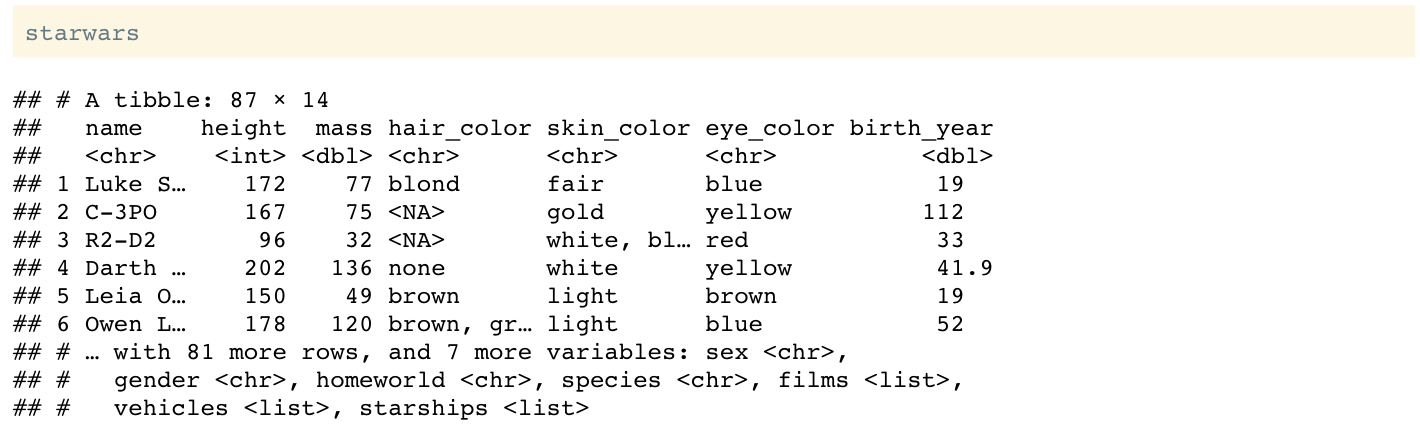
\includegraphics[width=1\linewidth]{Images/S2/code/s1}

	\end{figure}
	
	\end{frame}
	%------------------------------------------------------------------%
	
	
	\begin{frame}

		\frametitle{\textbf{Luke Skywalker}}
		
\begin{figure}
	\centering
	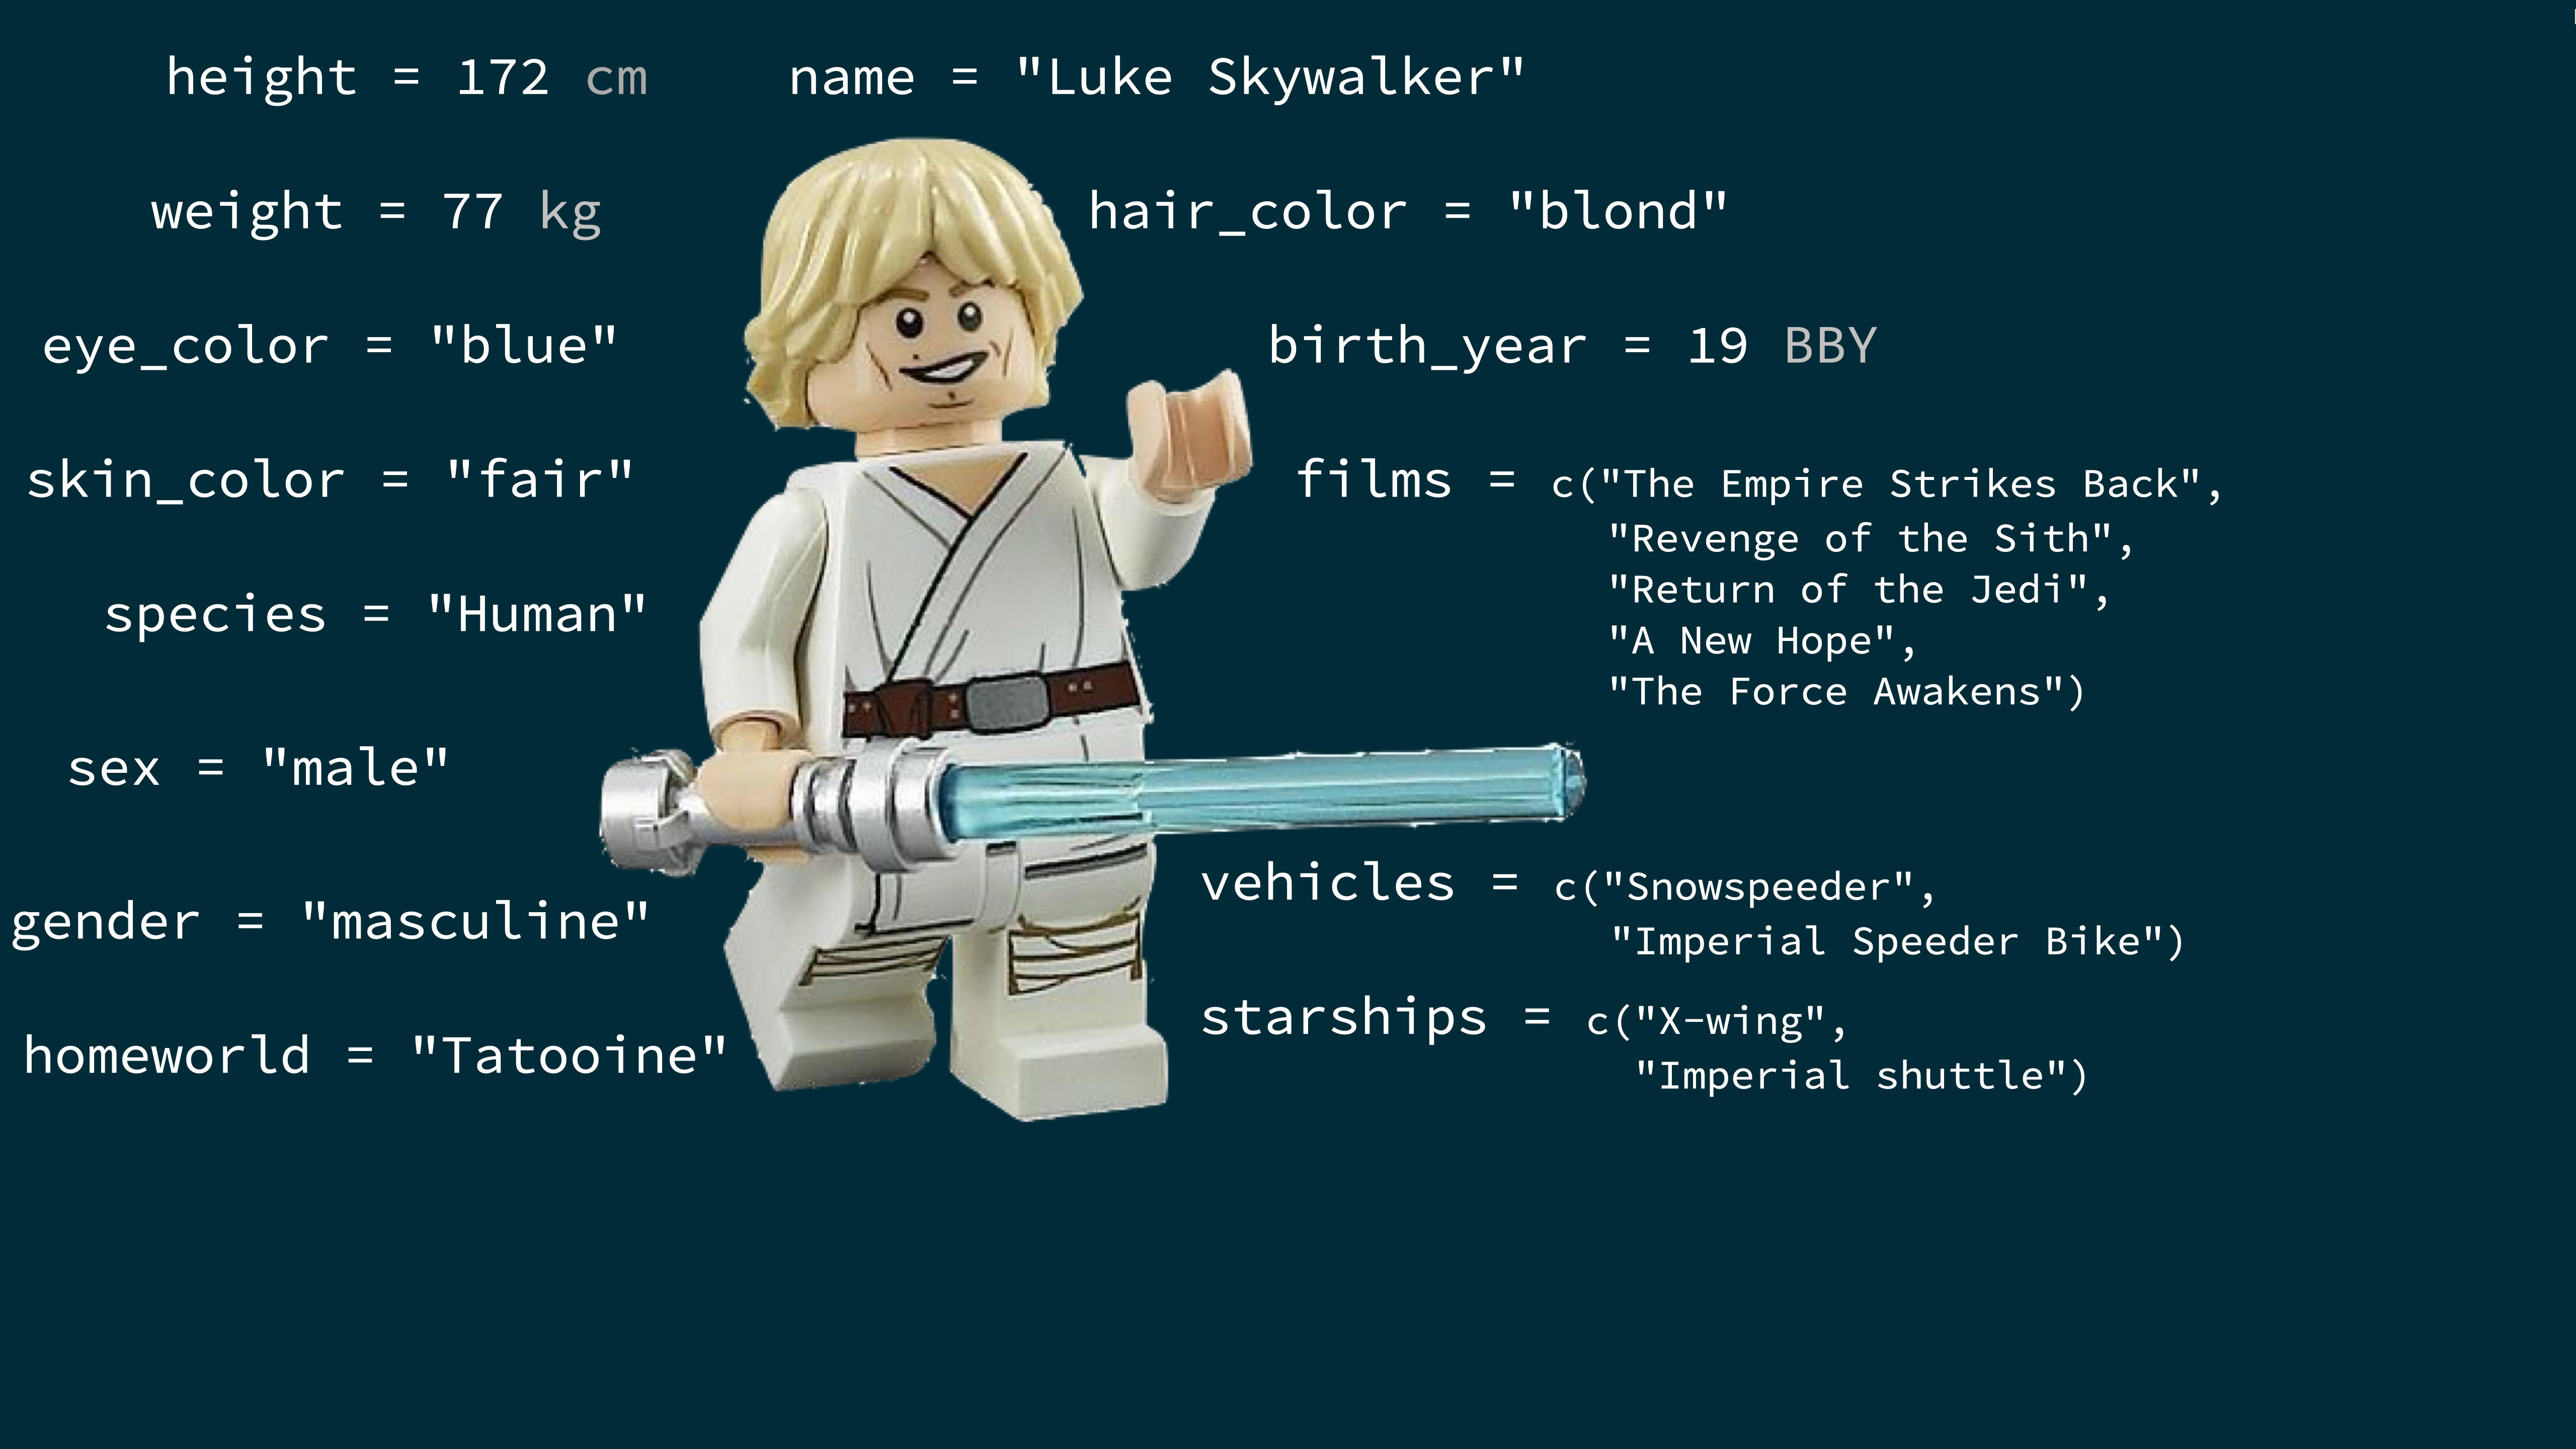
\includegraphics[width=0.8\linewidth]{Images/S2/luke-skywalker}

\end{figure}
	
	\end{frame}
	%------------------------------------------------------------------%
	
		%------------------------------------------------------------------%
	
	
	\begin{frame}
		
		\frametitle{\textbf{What's in the Star Wars Data?}}
		
		\begin{figure}
			\centering
			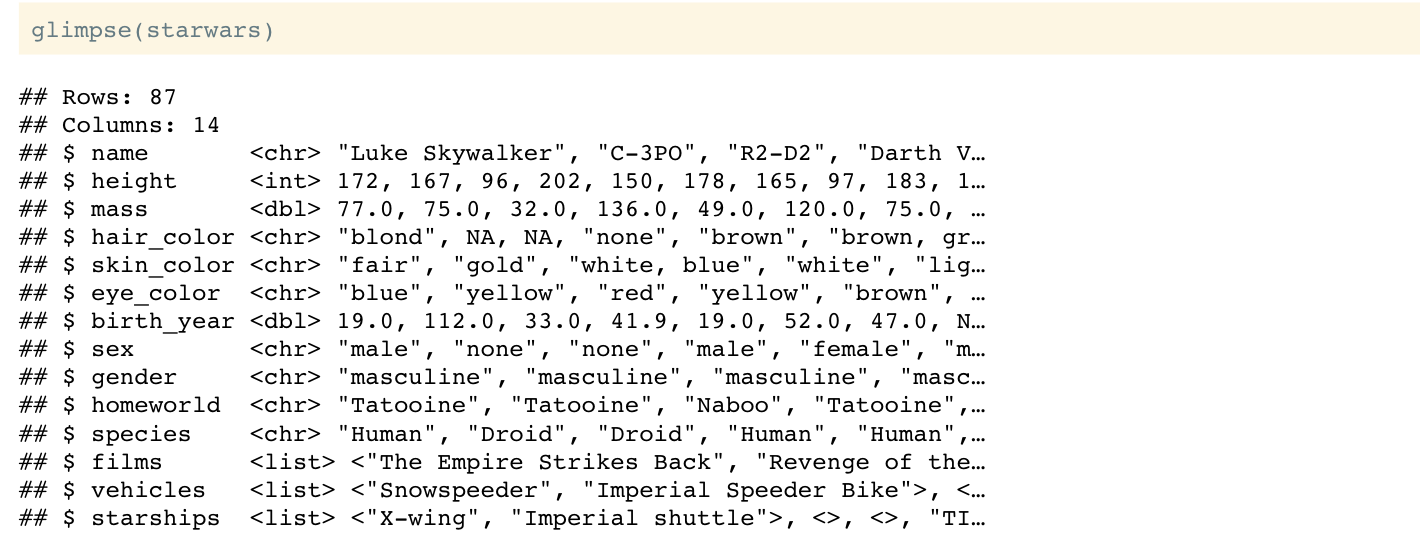
\includegraphics[width=1\linewidth]{Images/S2/code/s2}
			
		\end{figure}
		\small{How many rows and columns does this dataset have? What does each row represent? What does each column represent?}
		
		
	\end{frame}
	%------------------------------------------------------------------%
	
	
	
	\begin{frame}
		
		\frametitle{\textbf{Exploratory Data Analysis}}
		
	\begin{itemize}
		\item Exploratory data analysis (EDA) is an approach to analysing data sets to summarize its main characteristics
		\item Often, this is visual -- this is what we'll focus on first
		\item But we might also calculate summary statistics and perform data wrangling/manipulation/transformation at (or before) this stage of the analysis -- this is what we'll focus on next
	\end{itemize}
		
	\end{frame}
	%------------------------------------------------------------------%
		\begin{frame}
		
		\frametitle{\textbf{Mass vs. Height}}\vspace{-.5em}
		How would you describe the relationship between mass and height of Starwars characters? Who is the not so tall but really chubby character? Jabba!
		\vspace{-2em}
\begin{figure}
	\centering
	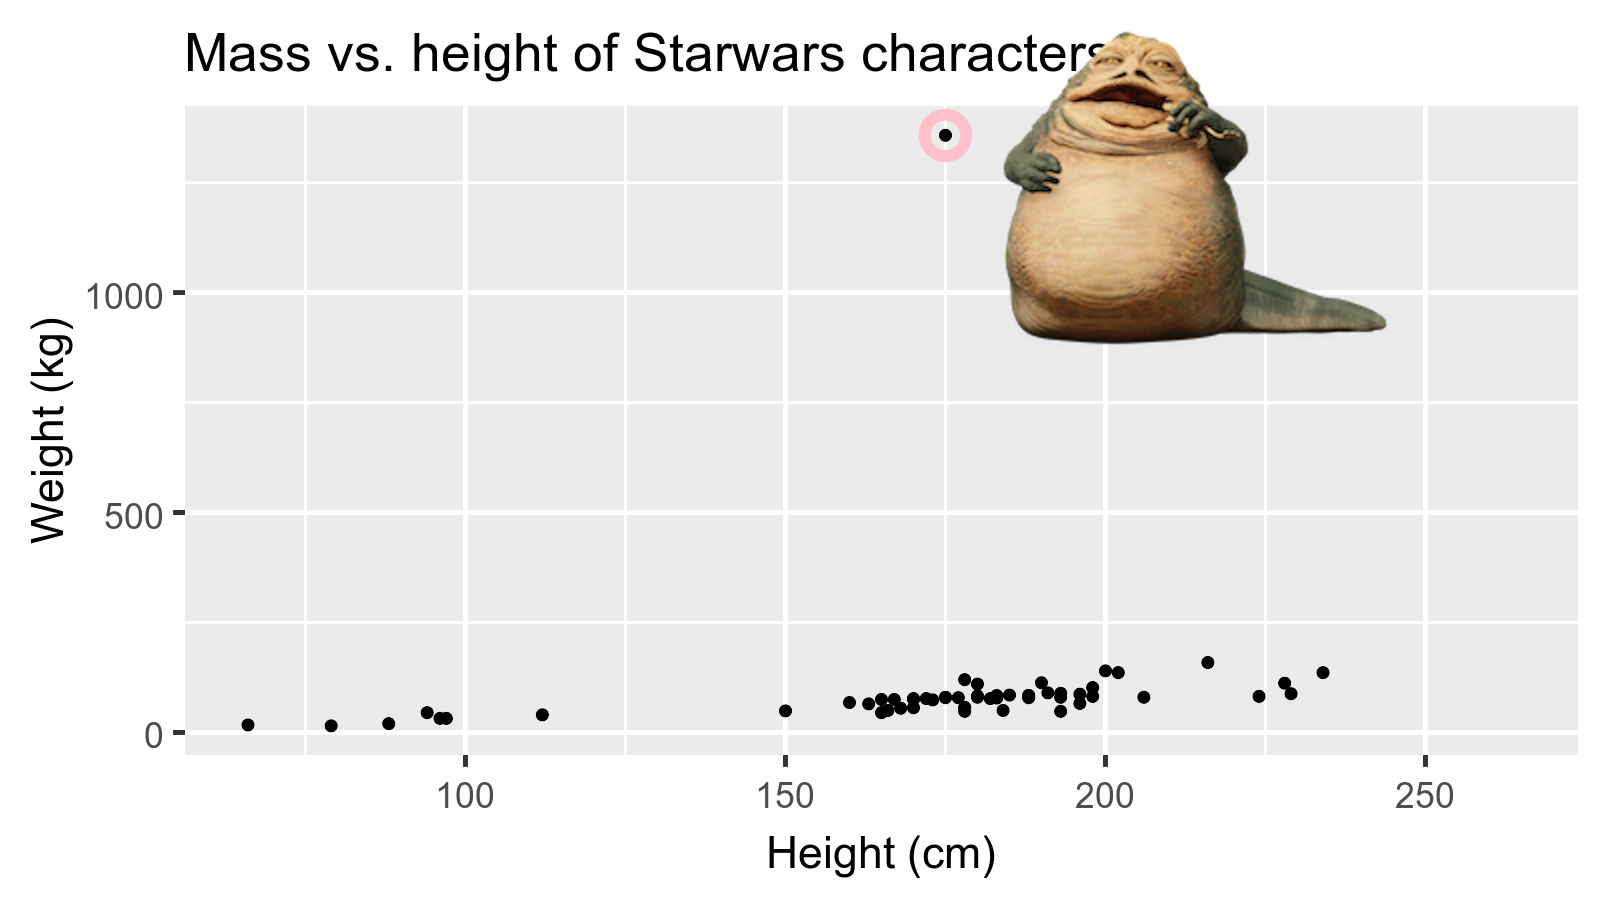
\includegraphics[width=0.75\linewidth]{Images/S2/jabbaplot}

\end{figure}

		
	\end{frame}
	%------------------------------------------------------------------%
	
			\begin{frame}
		
		\frametitle{\textbf{Data Visualization}}

			\begin{minipage}[t]{0.5\linewidth}
			\vspace{-1em}
				\begin{itemize}
				\item Data visualization is the creation and study of the visual representation of data
				\item Many tools for visualizing data -- R is one of them
				\item Many approaches/systems within R for making data visualizations -- \structure{ggplot2} is one of them, and that's what we're going to use
			\end{itemize}
		\end{minipage}%
		\begin{minipage}[t]{0.5\linewidth}
			\vspace{-3em}
			\begin{figure}
				\centering
				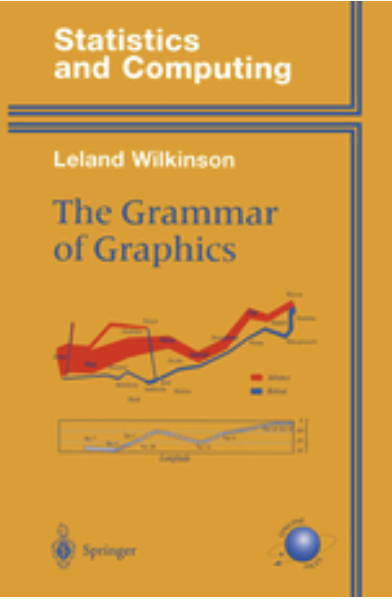
\includegraphics[width=0.35\linewidth]{Images/S2/grammar-of-graphics1}
				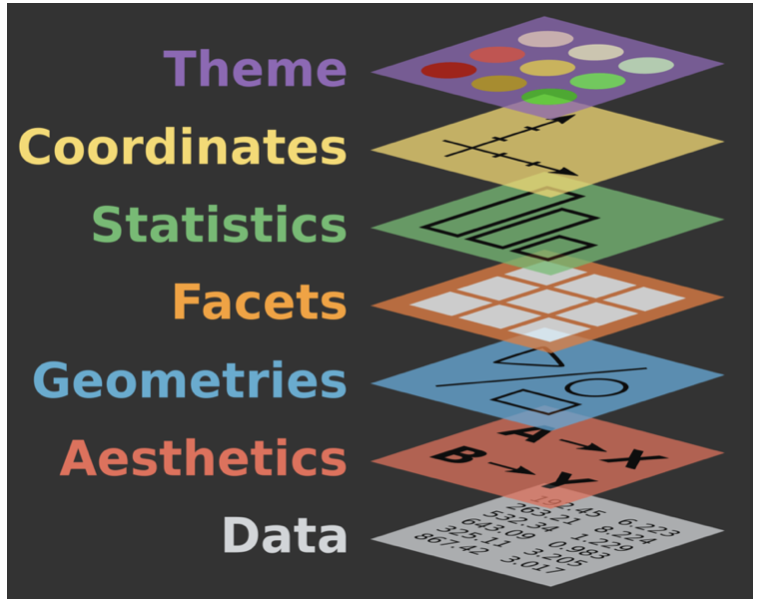
\includegraphics[width=0.7\linewidth]{Images/S2/grammar-of-graphics2}
		
			\end{figure}
	 
			
		\end{minipage}
	\end{frame}
	%------------------------------------------------------------------%
	%------------------------------------------------------------------%
	\begin{frame}
		
		\frametitle{\textbf{Mass vs. Height}}
		
		\begin{itemize}
			\item What are the functions doing the plotting?
			\item What is the dataset being plotted?
			\item Which variables map to which features (aesthetics) of the plot?
			\item What does the warning mean?
		\end{itemize}
		\begin{figure}
		\centering
		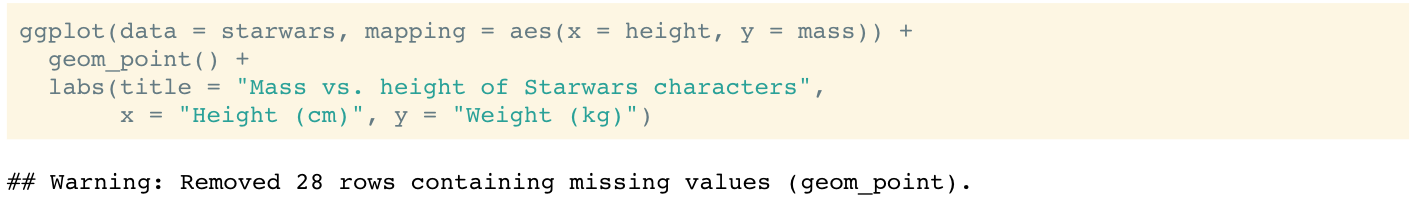
\includegraphics[width=1\linewidth]{Images/S2/code/s3}

		
	\end{figure}
	\end{frame}
	%------------------------------------------------------------------%
	
		\begin{frame}
		
		\frametitle{\textbf{Visualising Data with ggplot2}}
		
\begin{itemize}
	\item ggplot2 is tidyverse's data visualization package
	\item Structure of the code for plots can be summarized as:
\end{itemize}
\begin{figure}
	\centering
	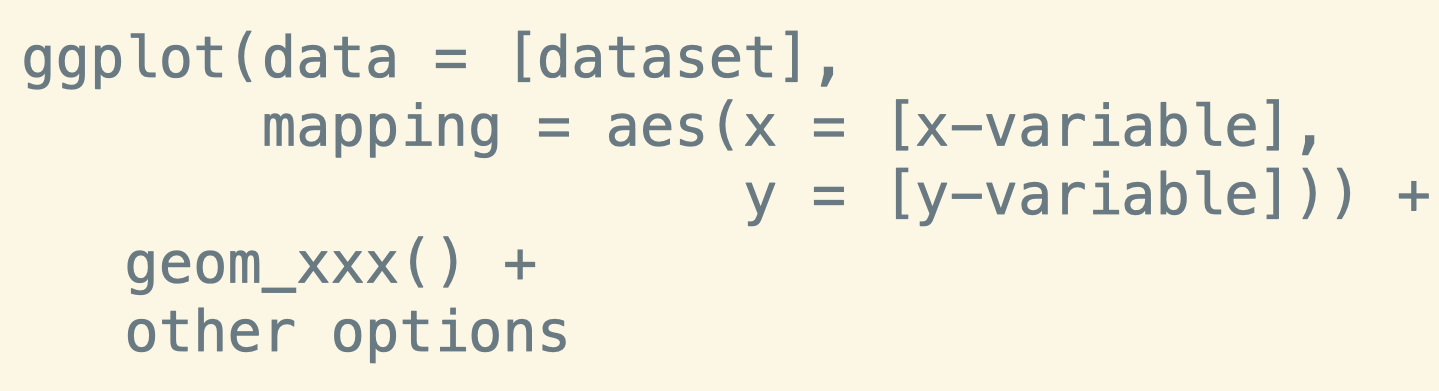
\includegraphics[width=0.5\linewidth]{Images/S2/code/s4}

\end{figure}
\textbf{Data: Palmer Penguins}. Measurements for penguin species, island in Palmer Archipelago, size (flipper length, body mass, bill dimensions), and sex.
\begin{figure}
	\centering
	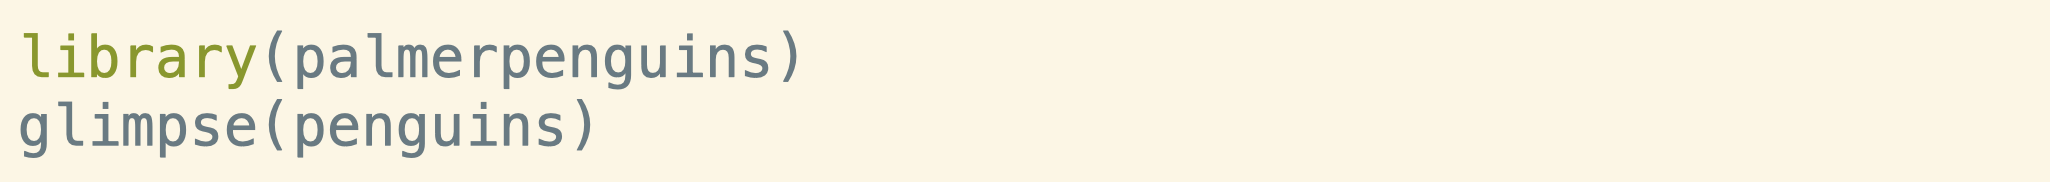
\includegraphics[width=0.7\linewidth]{Images/S2/code/s5}
	
\end{figure}

	\end{frame}
	%------------------------------------------------------------------%
	
		
	\begin{frame}
		
		\frametitle{\textbf{Visualising Data with ggplot2}}

		\begin{figure}
			\centering
			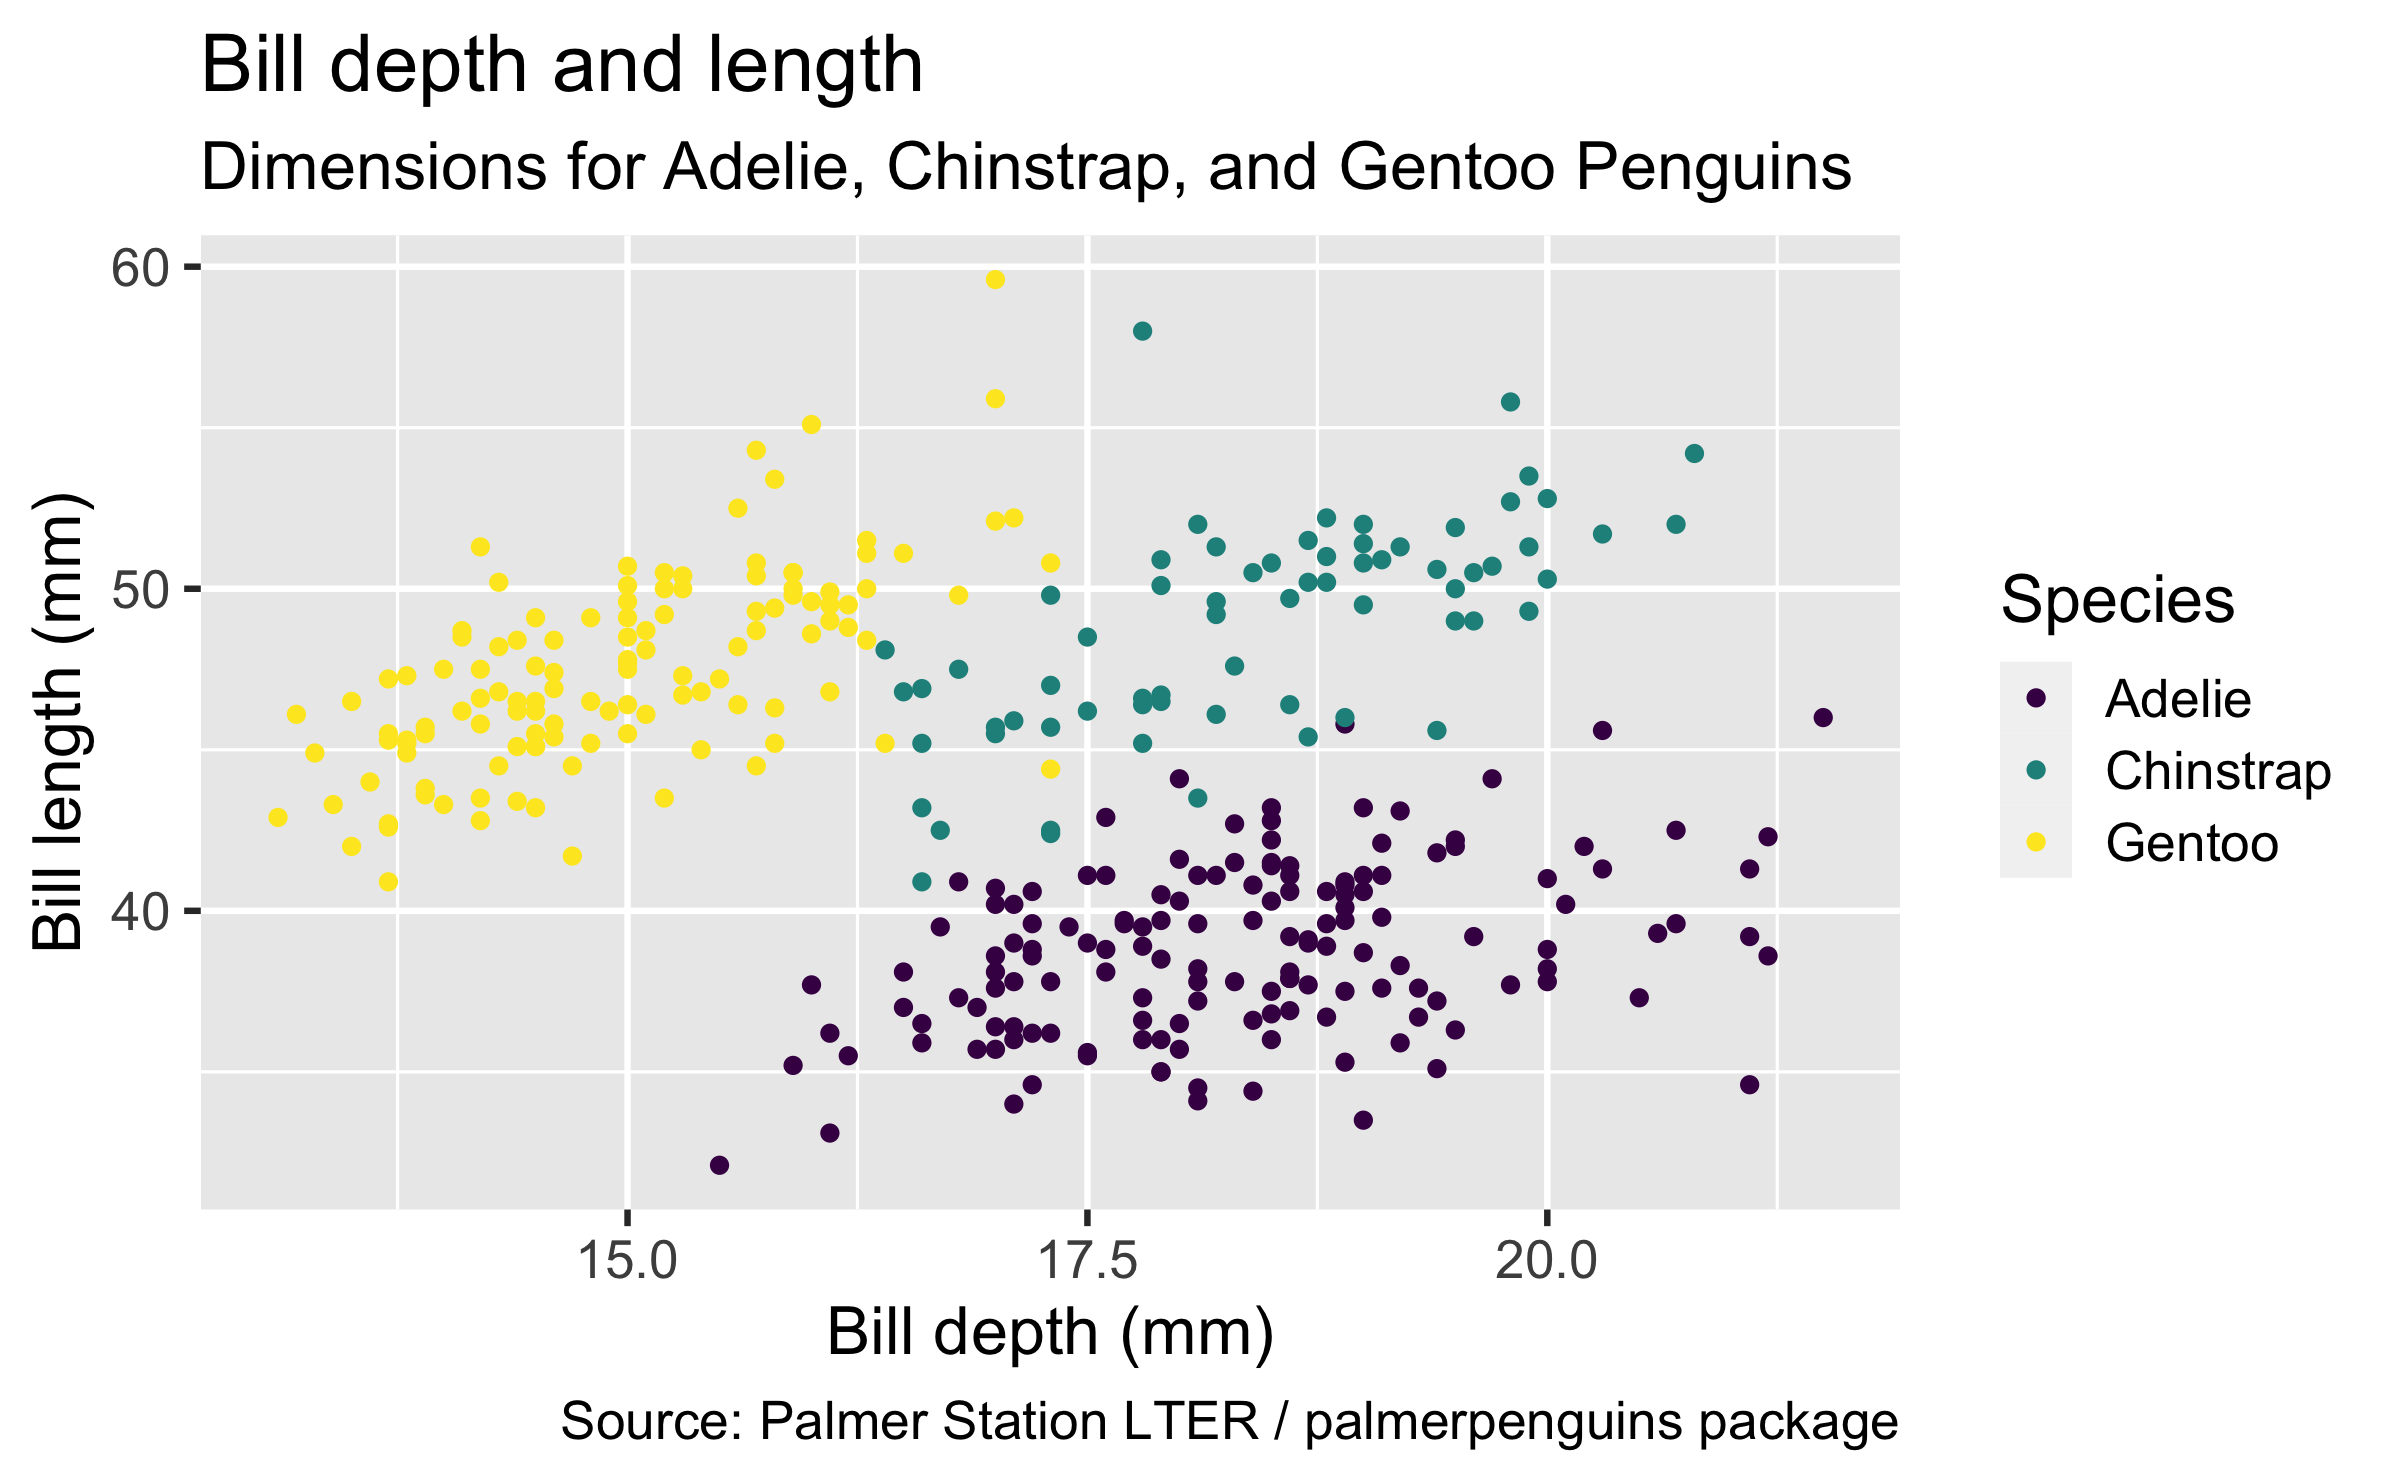
\includegraphics[width=.8\linewidth]{Images/S2/penguins-10-nohighlight-1}
			
		\end{figure}
\
		
	\end{frame}

	%------------------------------------------------------------------%
	
	\begin{frame}

		\frametitle{\textbf{Coding Out Loud}}
\structure{Start with the penguins data frame}

			\begin{minipage}[t]{0.5\linewidth}
	\begin{figure}
	\centering
	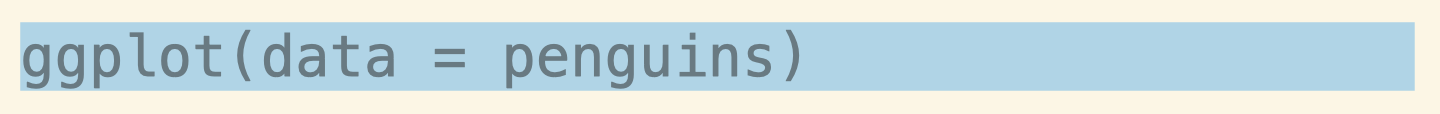
\includegraphics[width=1\linewidth]{Images/S2/code/s6}
	
\end{figure}
\end{minipage}%
\begin{minipage}[t]{0.5\linewidth}

	\begin{figure}
		\centering
		
\includegraphics[width=1\linewidth]{Images/S2/penguins-0-1}
		
	\end{figure}
	
	
\end{minipage}
		
	\end{frame}
	%------------------------------------------------------------------%
	
		\begin{frame}
		

		Start with the penguins data frame, \structure{map bill depth to the x-axis}
		
		\begin{minipage}[t]{0.5\linewidth}
			\begin{figure}
				\centering
				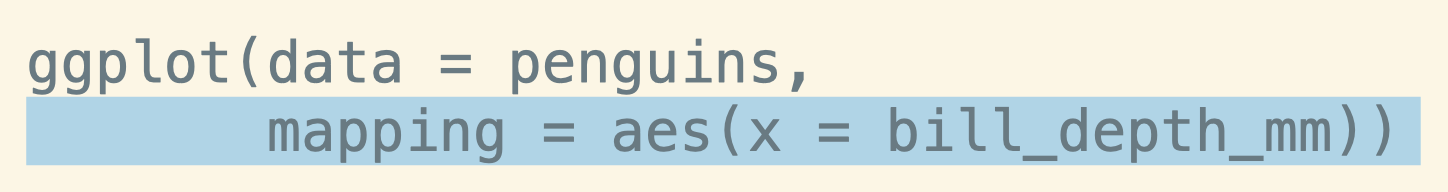
\includegraphics[width=1\linewidth]{Images/S2/code/s7}
				
			\end{figure}
		\end{minipage}%
		\begin{minipage}[t]{0.5\linewidth}
			
			\begin{figure}
				\centering
				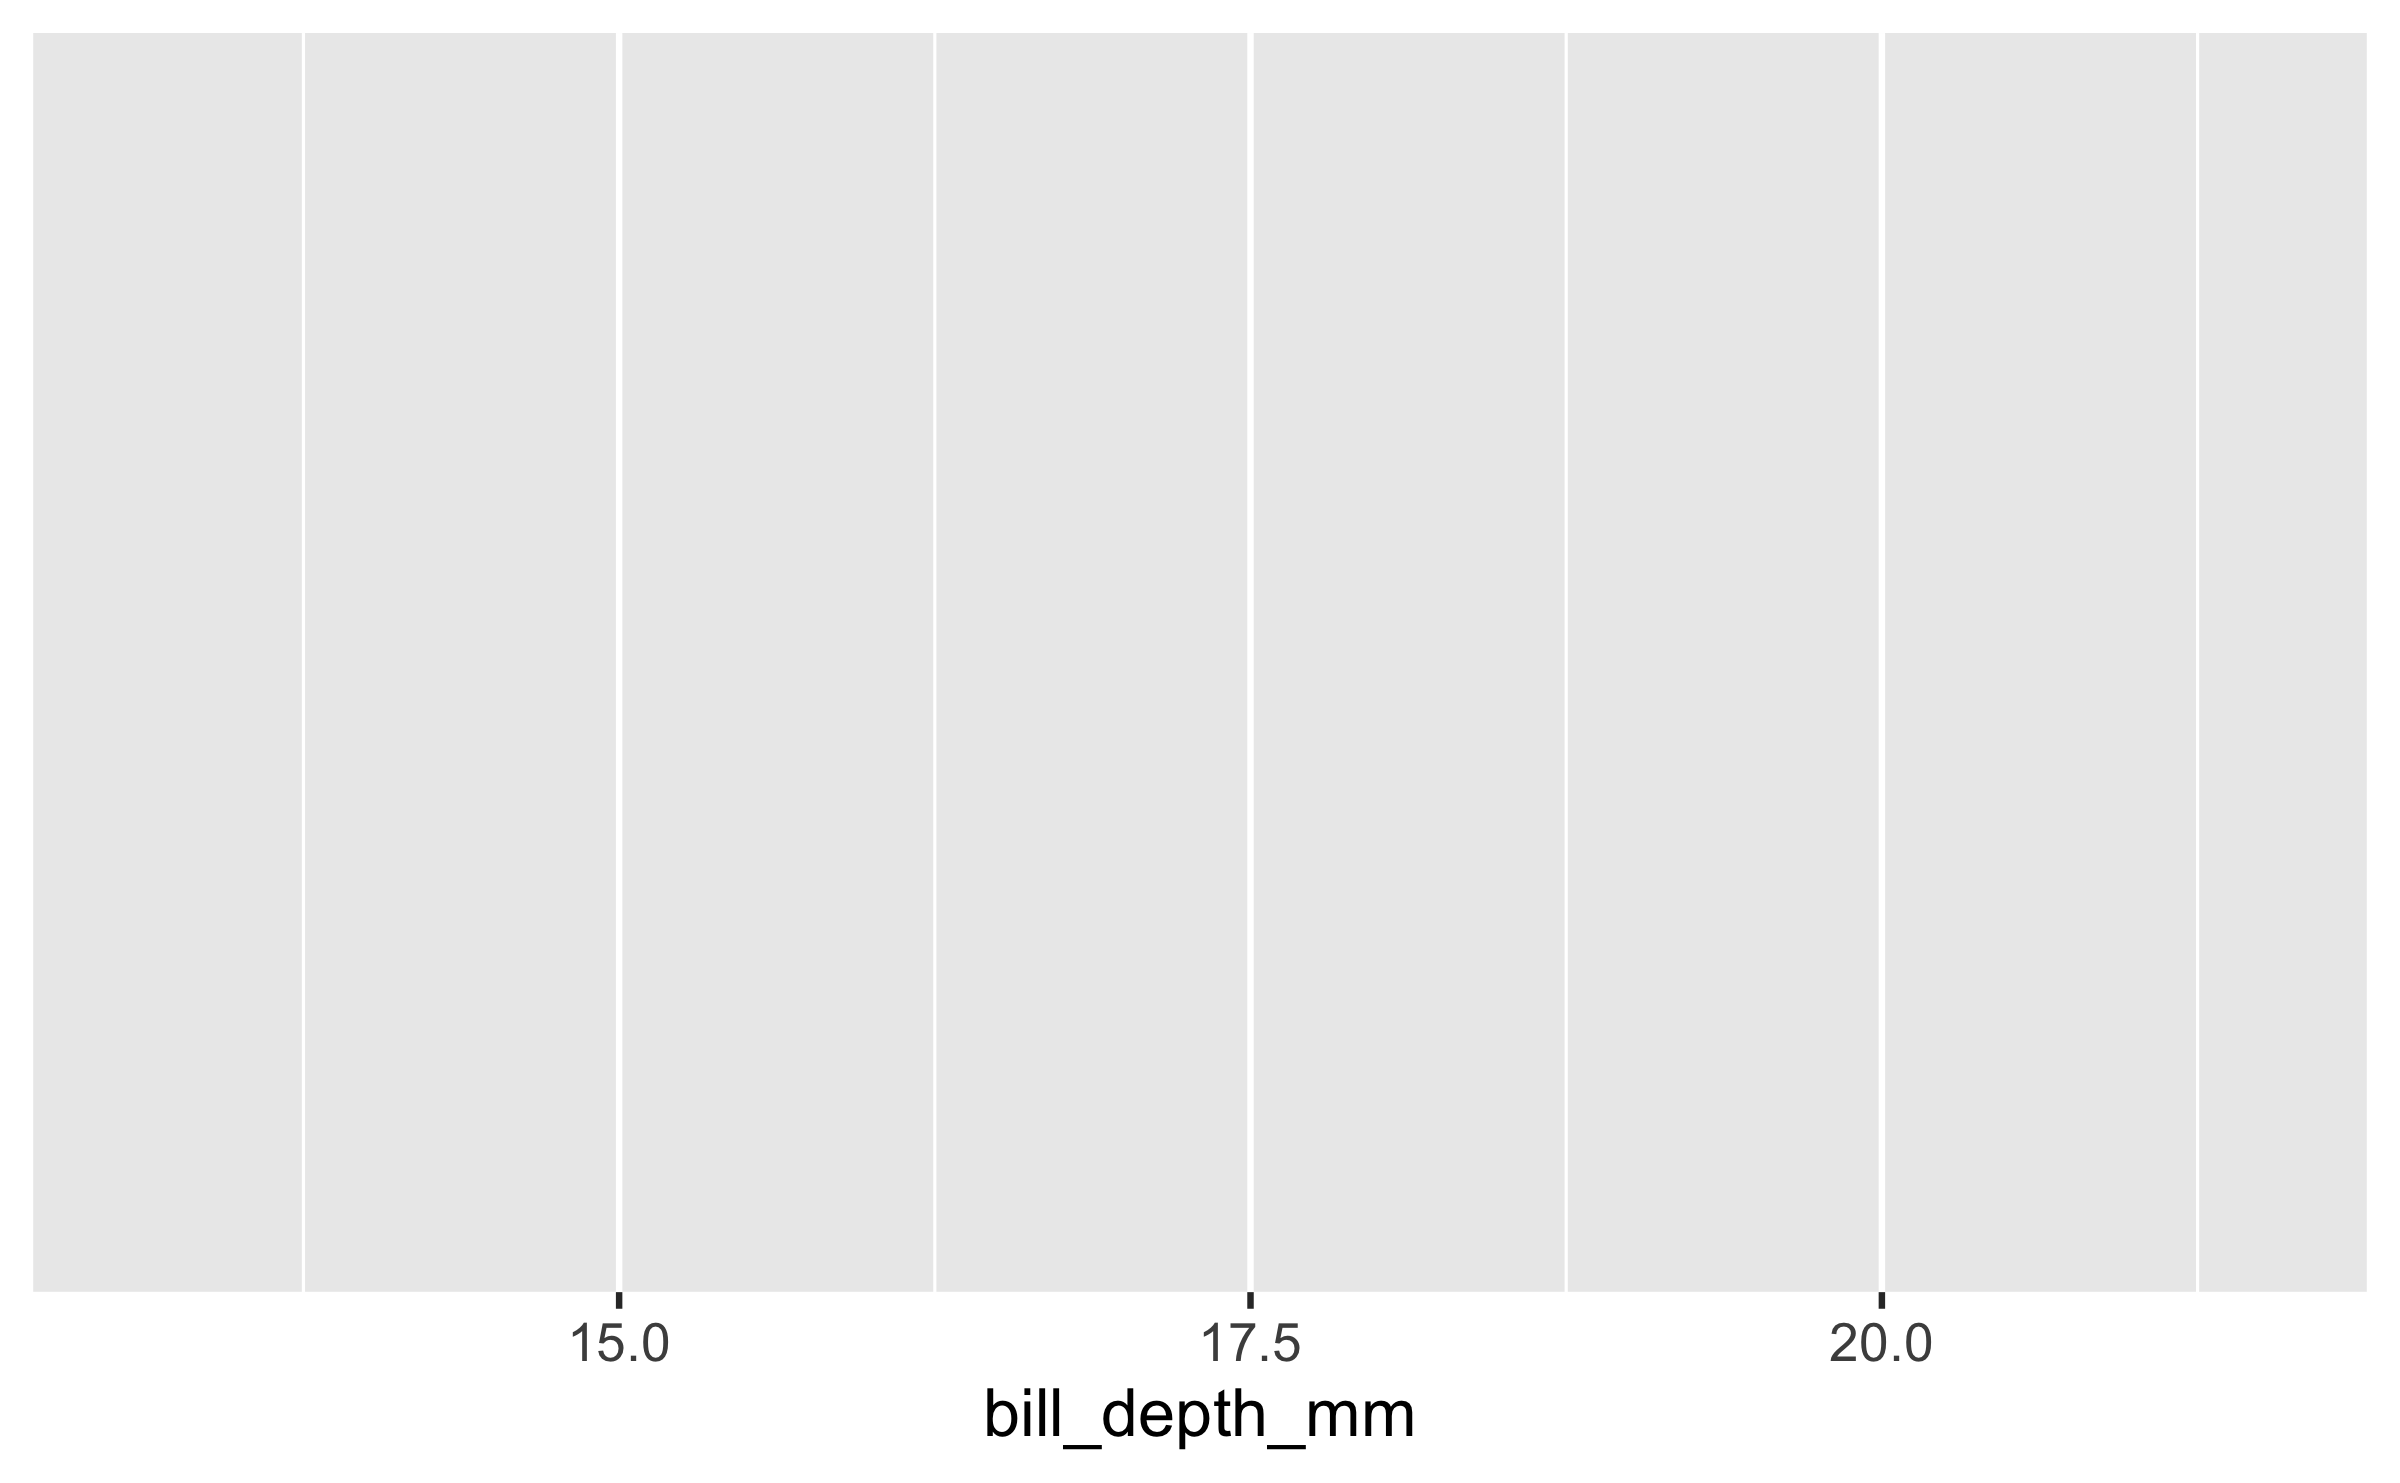
\includegraphics[width=1\linewidth]{Images/S2/penguins-1-1}
				
			\end{figure}
			
			
		\end{minipage}
		
	\end{frame}
	%------------------------------------------------------------------%
		%------------------------------------------------------------------%
	
	\begin{frame}
		

		Start with the penguins data frame, map bill depth to the x-axis \structure{and map bill length to the y-axis.}
		
		\begin{minipage}[t]{0.5\linewidth}
			\begin{figure}
				\centering
				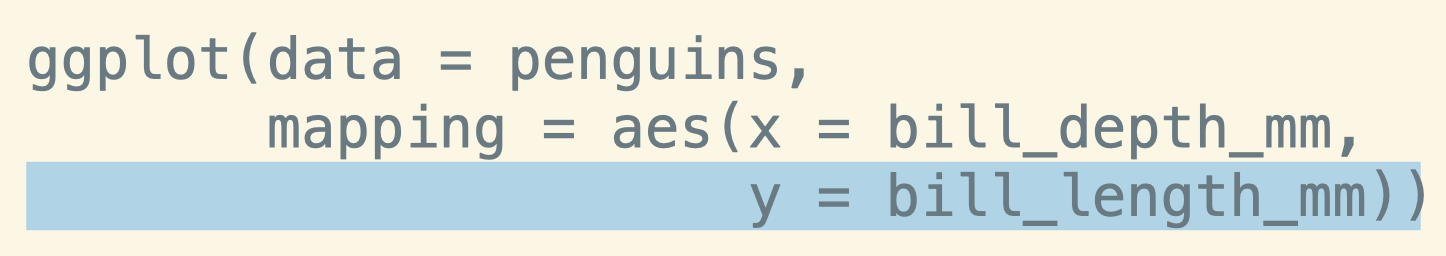
\includegraphics[width=1\linewidth]{Images/S2/code/s8}
				
			\end{figure}
		\end{minipage}%
		\begin{minipage}[t]{0.5\linewidth}
			
			\begin{figure}
				\centering
				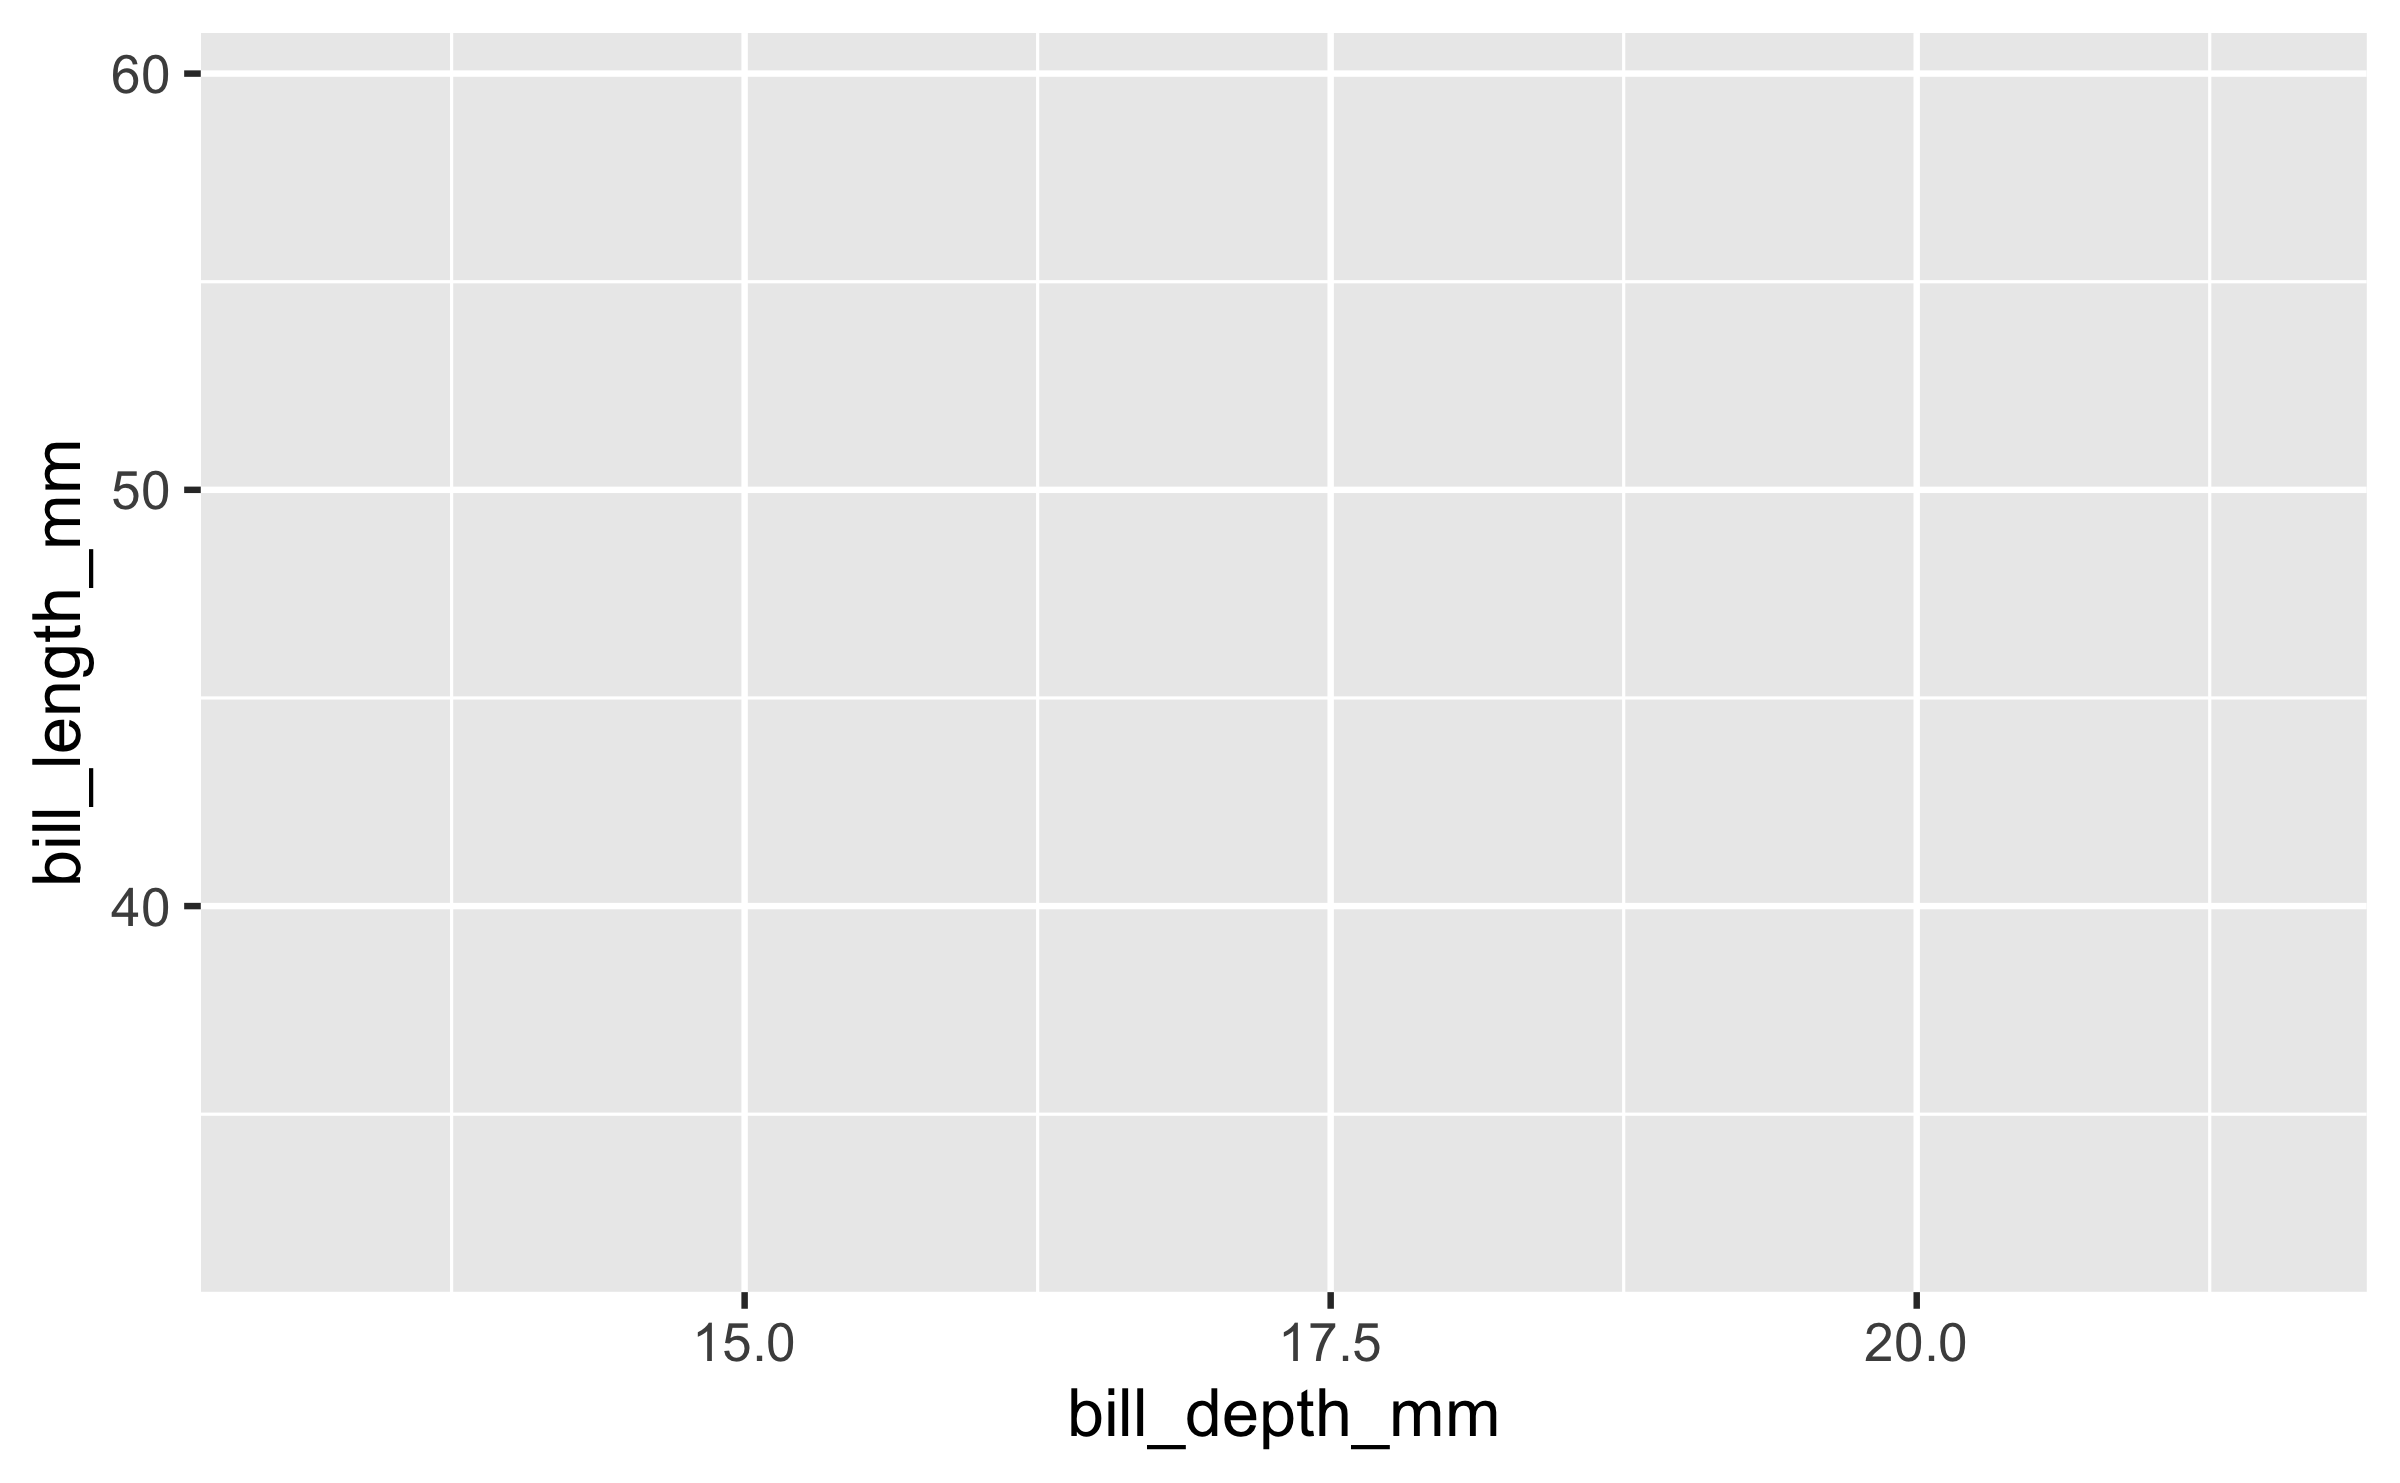
\includegraphics[width=1\linewidth]{Images/S2/penguins-2-1}
				
			\end{figure}
			
			
		\end{minipage}
		
	\end{frame}
	%------------------------------------------------------------------%
		\begin{frame}
		

		Start with the penguins data frame, map bill depth to the x-axis and map bill length to the y-axis. \structure{Represent each observation with a point}
		
		\begin{minipage}[t]{0.5\linewidth}
			\begin{figure}
				\centering
				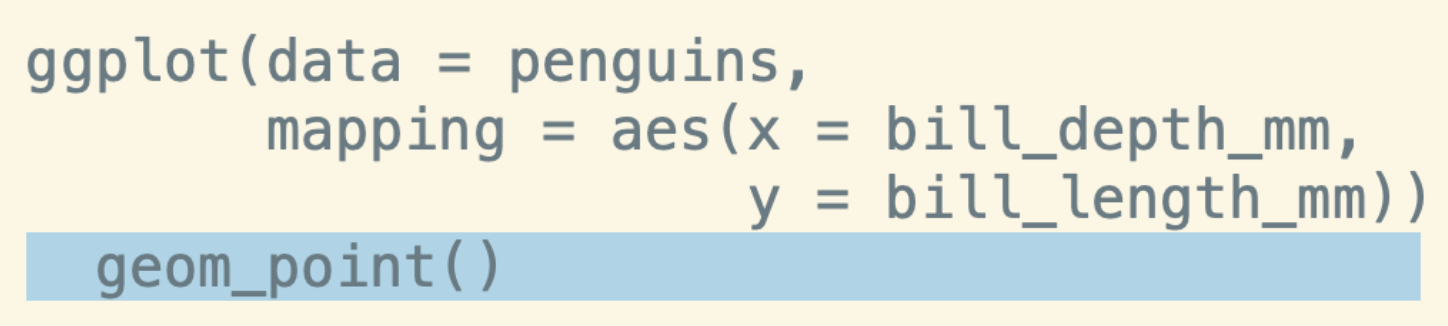
\includegraphics[width=1\linewidth]{Images/S2/code/s9}
				
			\end{figure}
		\end{minipage}%
		\begin{minipage}[t]{0.5\linewidth}
			
			\begin{figure}
				\centering
				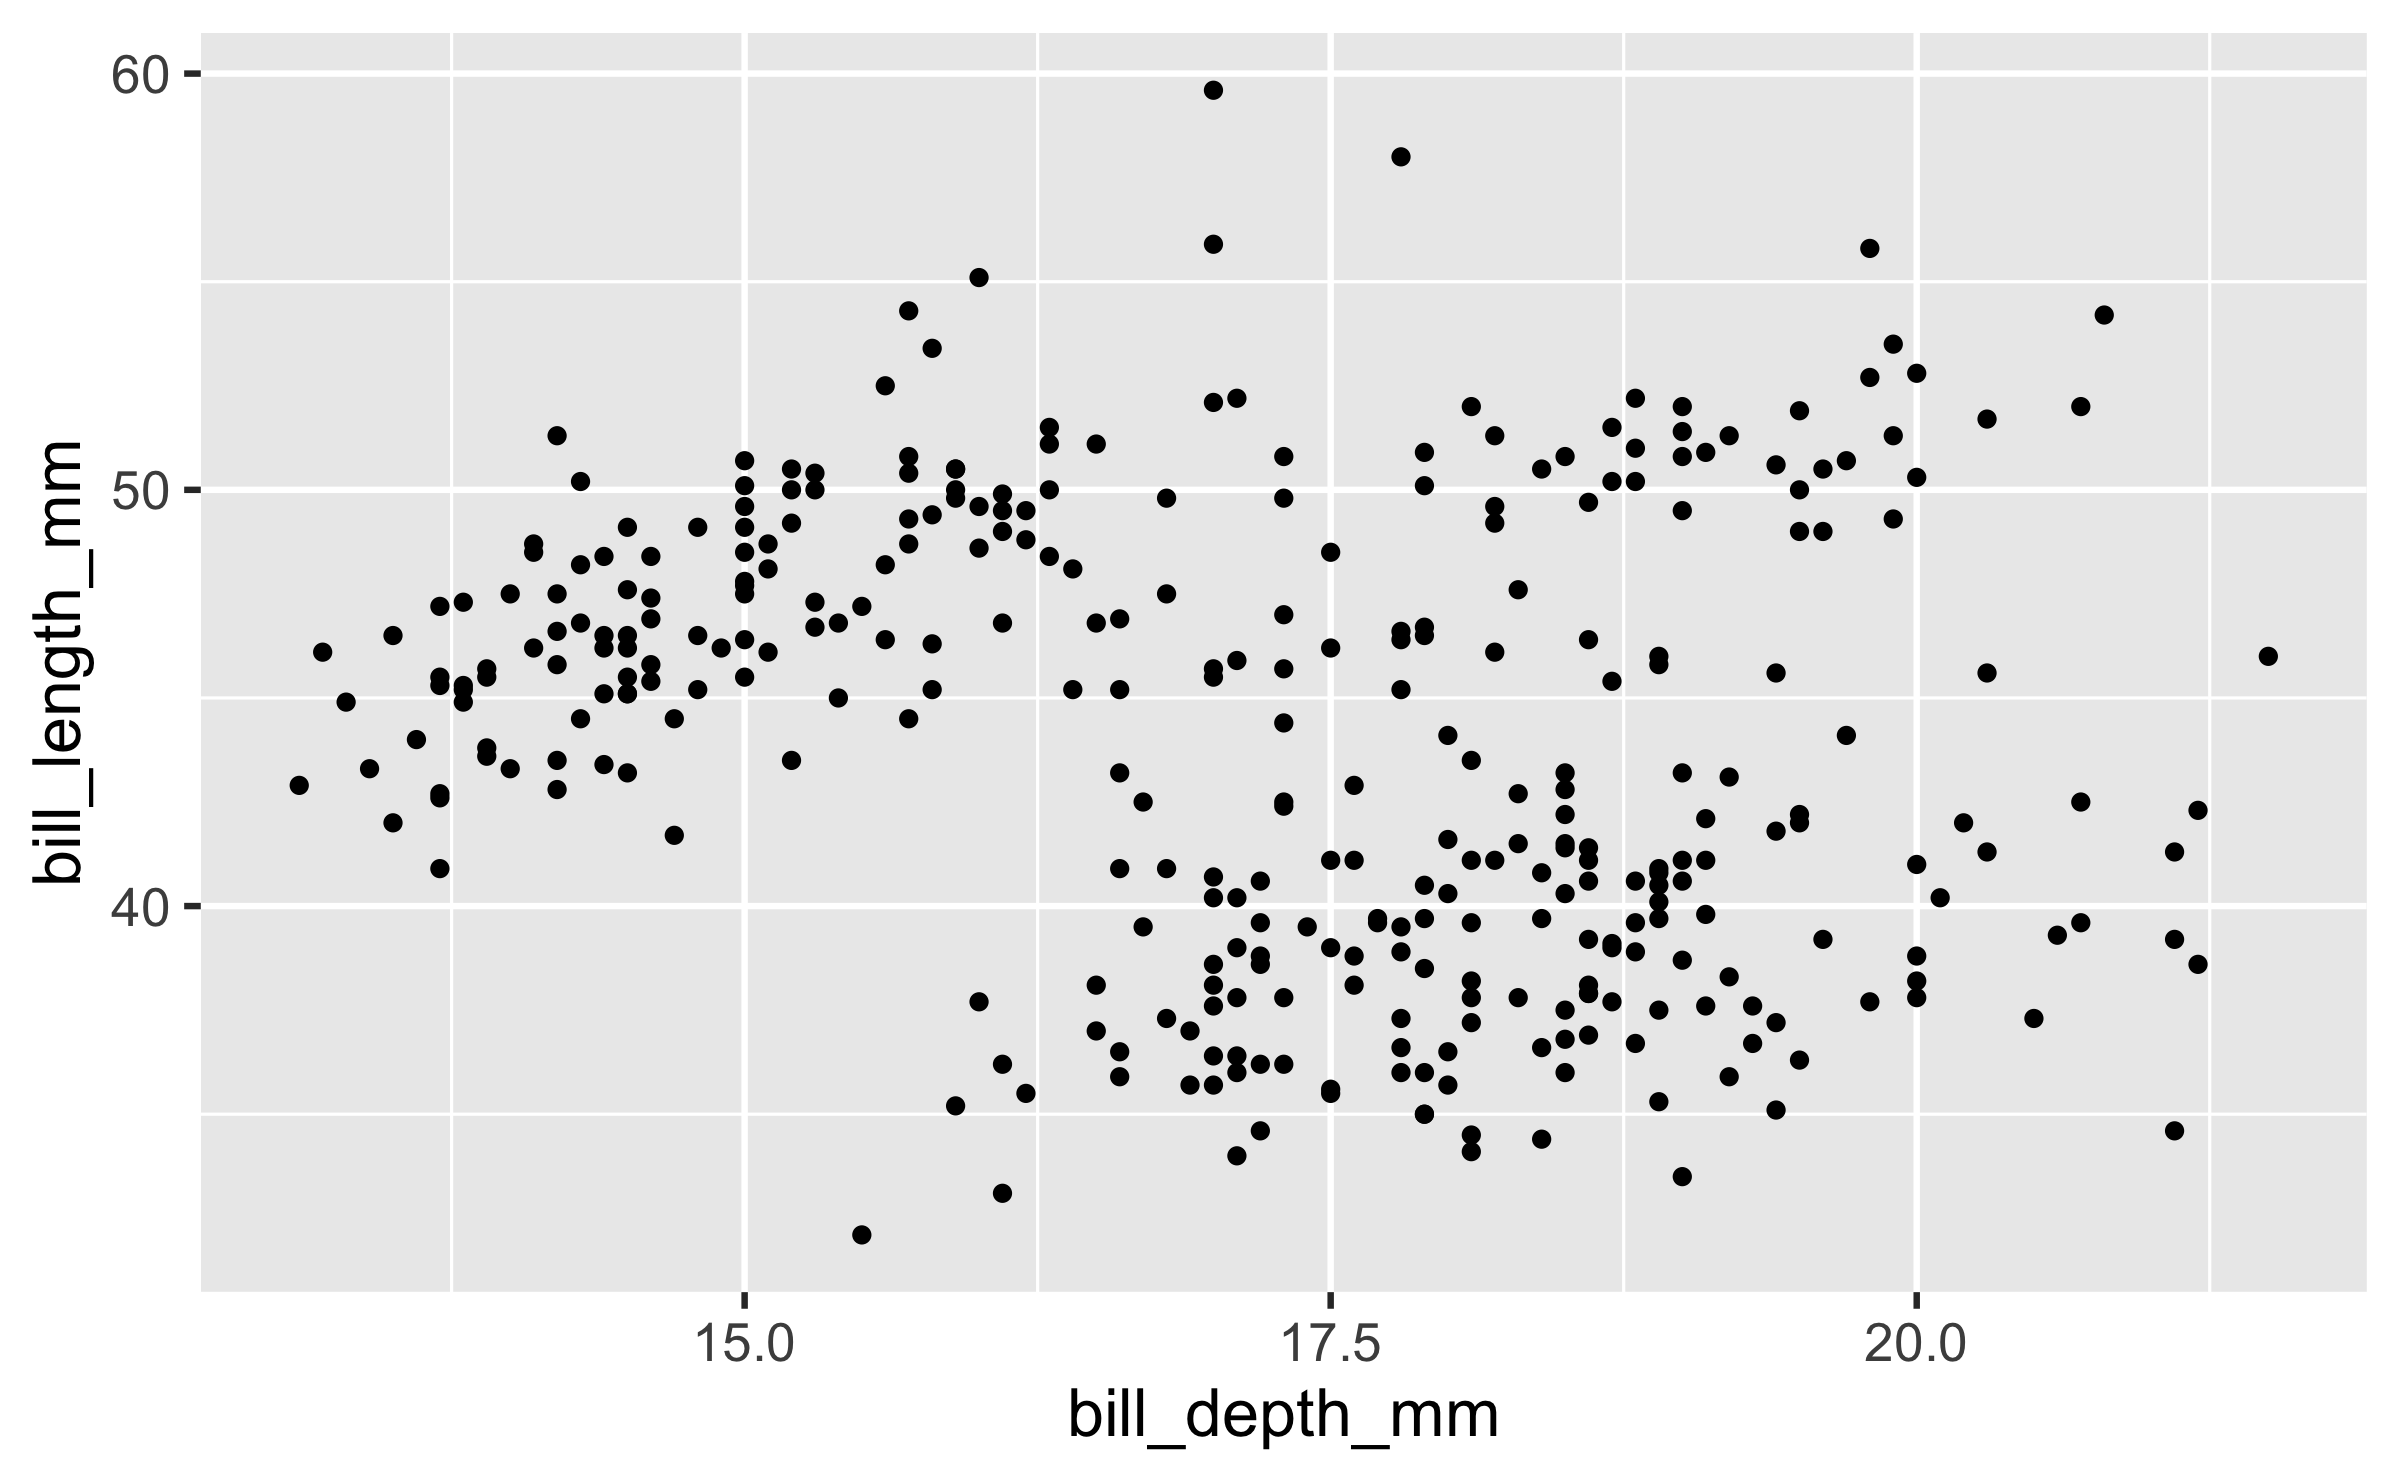
\includegraphics[width=1\linewidth]{Images/S2/penguins-3-1}
				
			\end{figure}
			
			
		\end{minipage}
		
	\end{frame}
		%------------------------------------------------------------------%

	\begin{frame}
	

	Start with the penguins data frame, map bill depth to the x-axis and map bill length to the y-axis. Represent each observation with a point \structure{and map species to the colour of each point.}
	
	\begin{minipage}[t]{0.5\linewidth}
		\begin{figure}
			\centering
			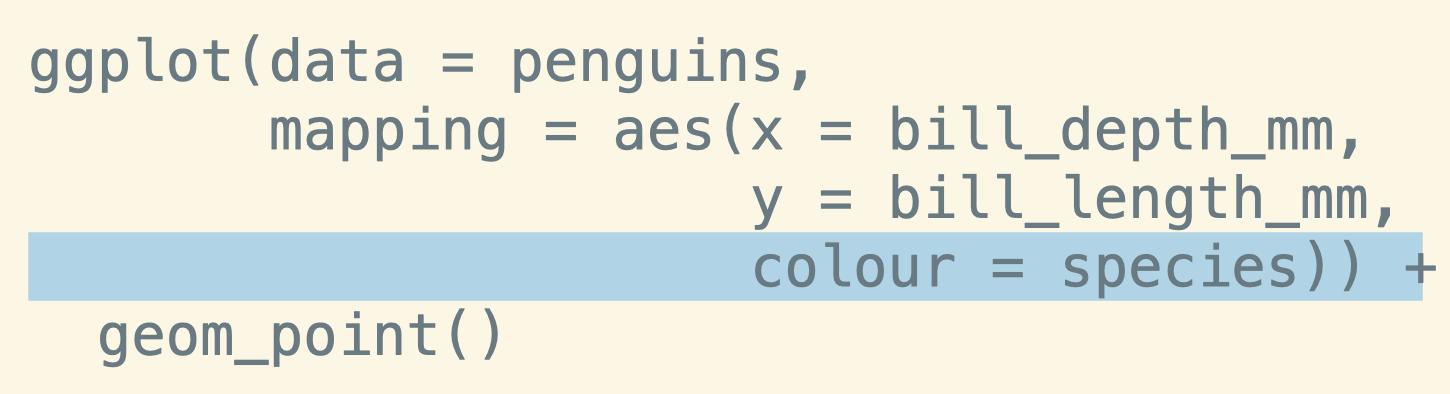
\includegraphics[width=1\linewidth]{Images/S2/code/s10}
			
		\end{figure}
	\end{minipage}%
	\begin{minipage}[t]{0.5\linewidth}
		
		\begin{figure}
			\centering
			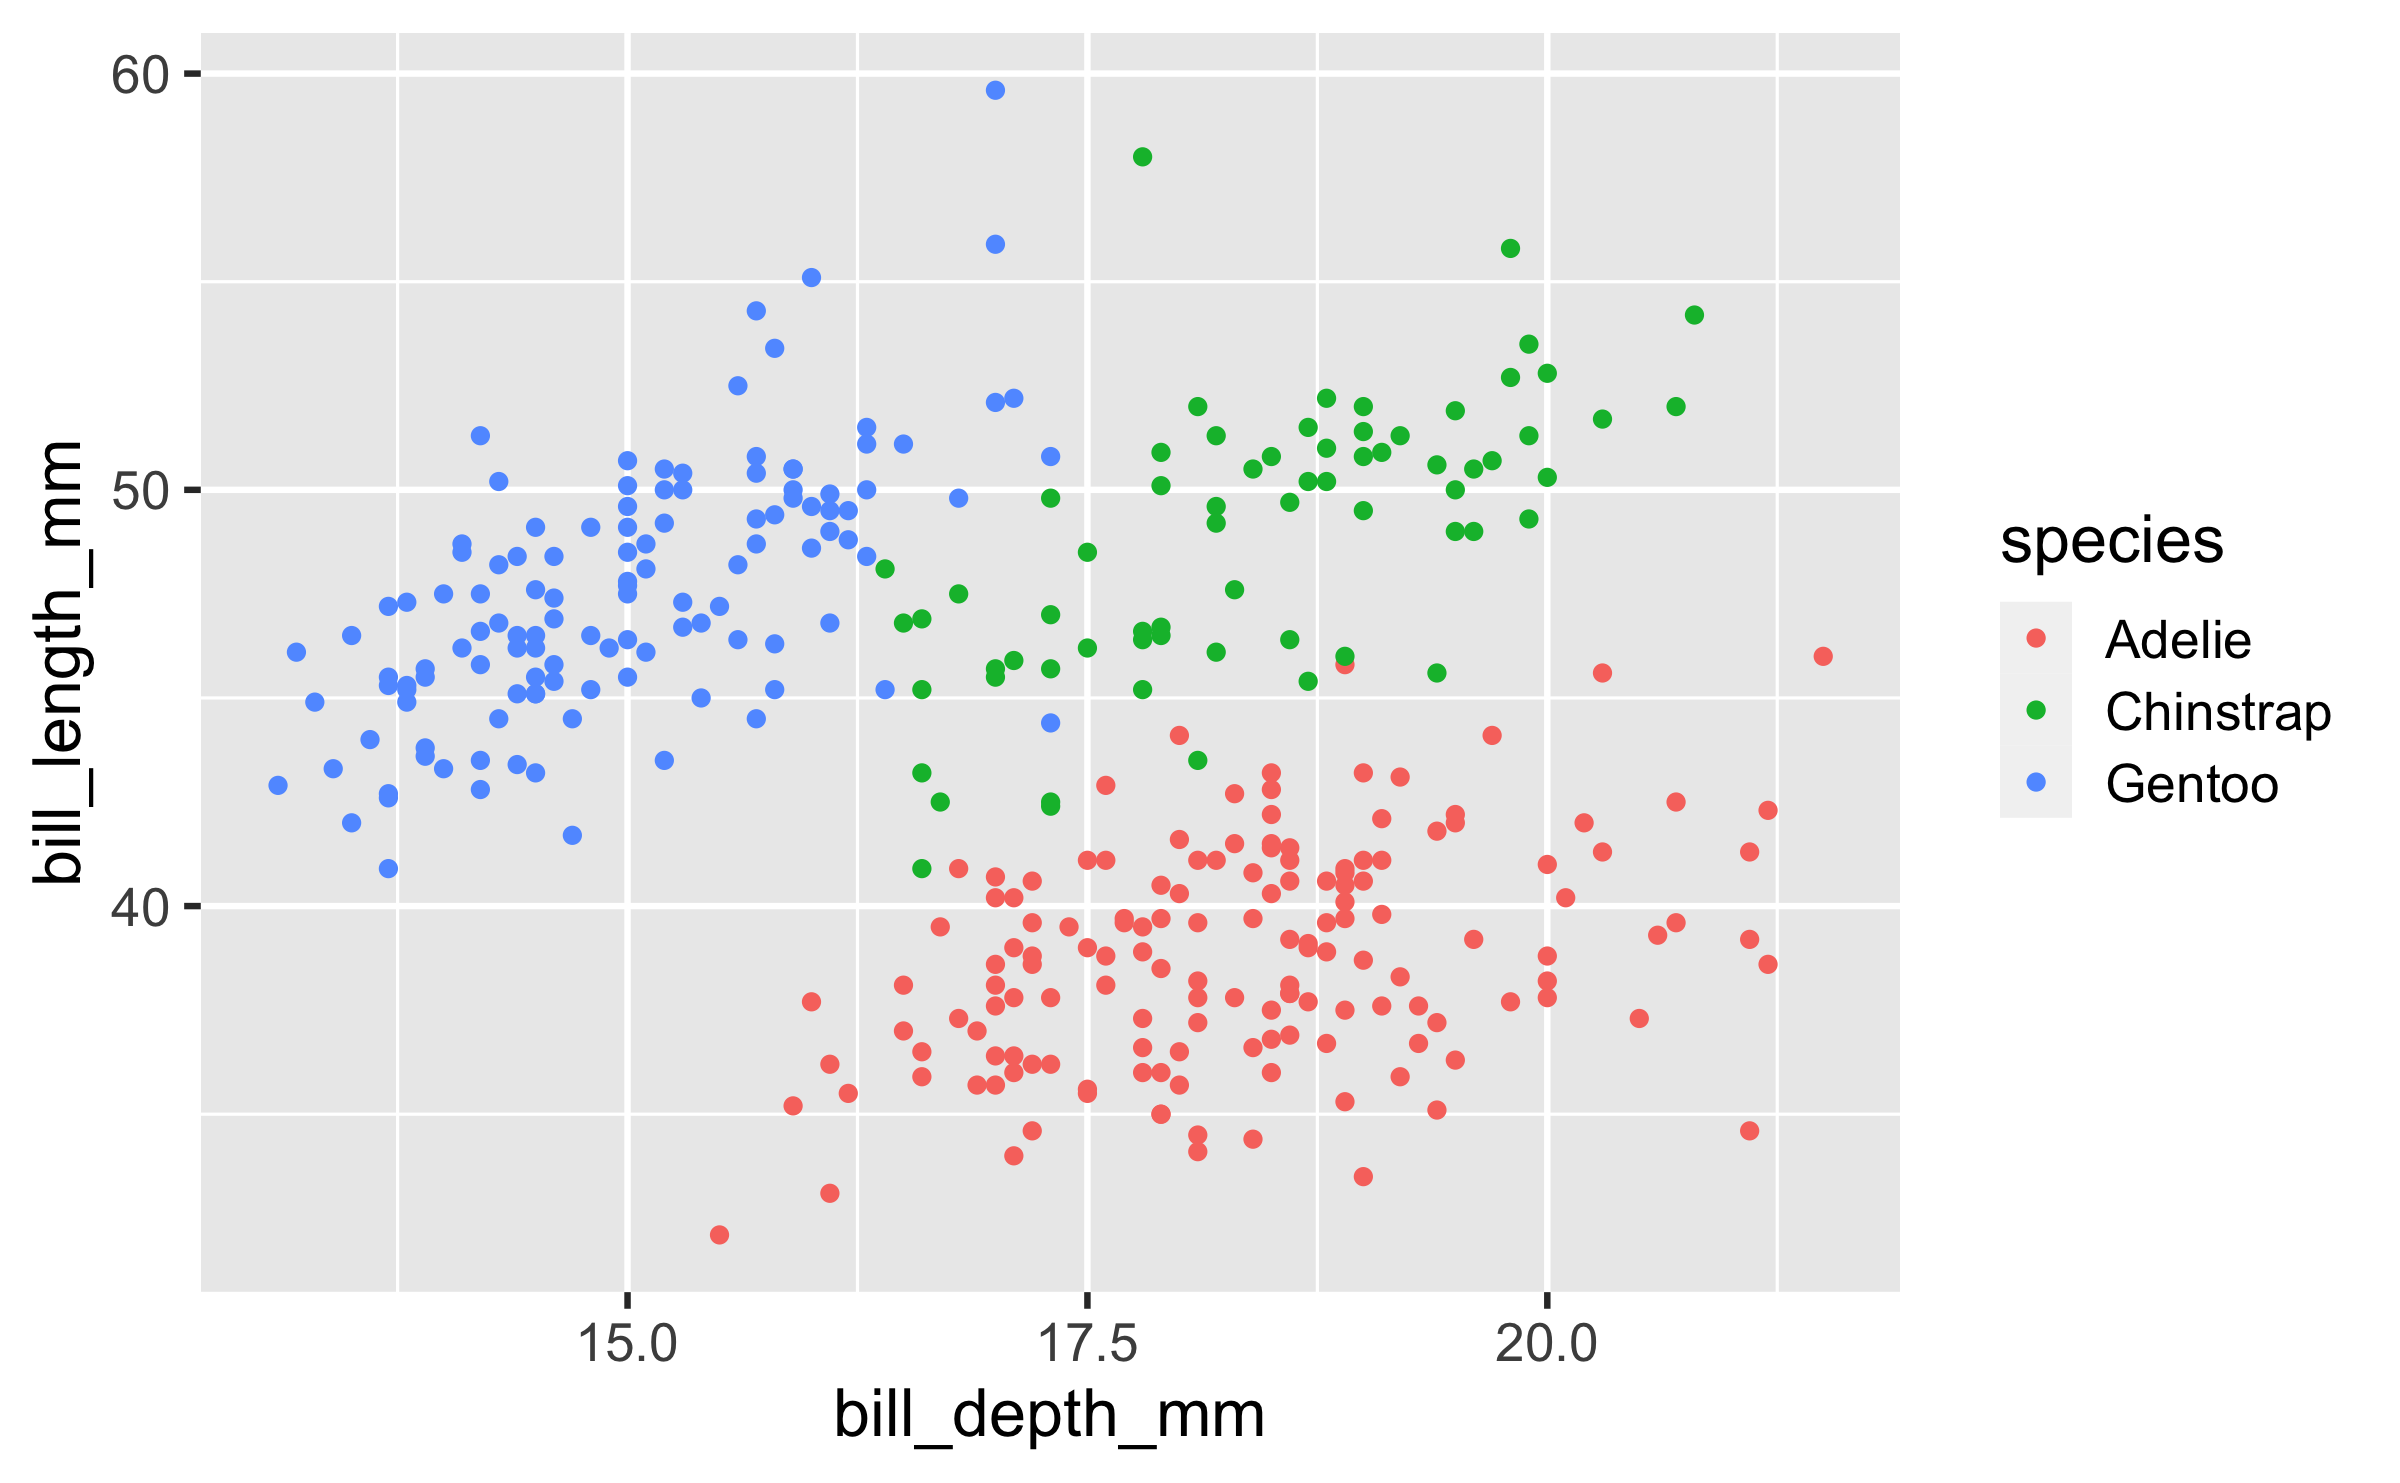
\includegraphics[width=1\linewidth]{Images/S2/penguins-4-1}
			
		\end{figure}
		
		
	\end{minipage}
	
\end{frame}
%------------------------------------------------------------------%

	\begin{frame}
	
	Start with the penguins data frame, map bill depth to the x-axis and map bill length to the y-axis. Represent each observation with a point and map species to the colour of each point. \structure{Title the plot "Bill depth and length"}
	
	\begin{minipage}[t]{0.5\linewidth}
		\begin{figure}
			\centering
			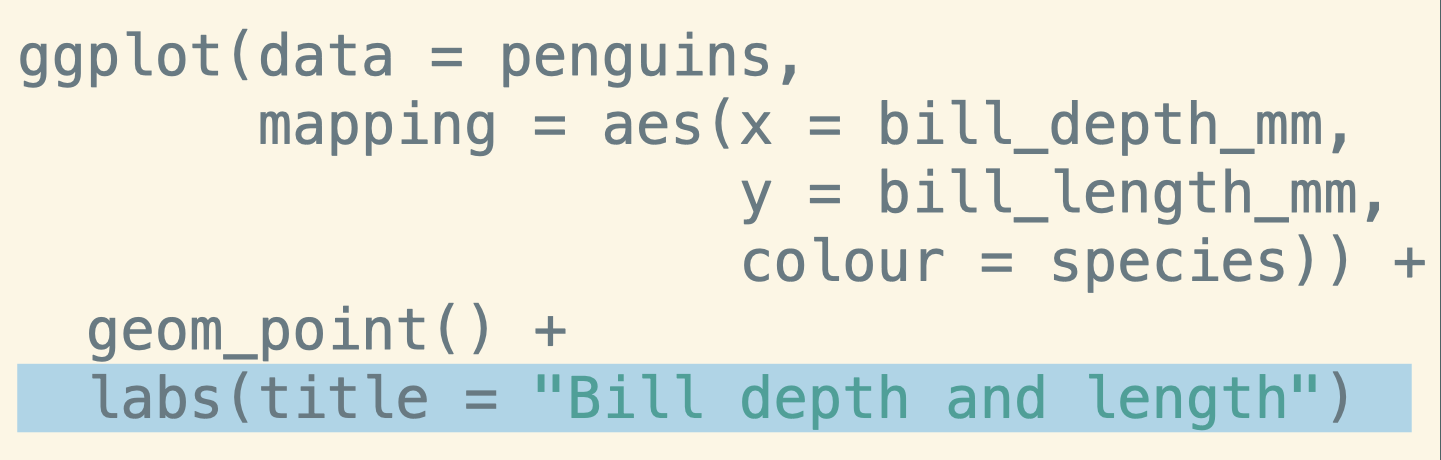
\includegraphics[width=1\linewidth]{Images/S2/code/s11}
			
		\end{figure}
	\end{minipage}%
	\begin{minipage}[t]{0.5\linewidth}
		
		\begin{figure}
			\centering
			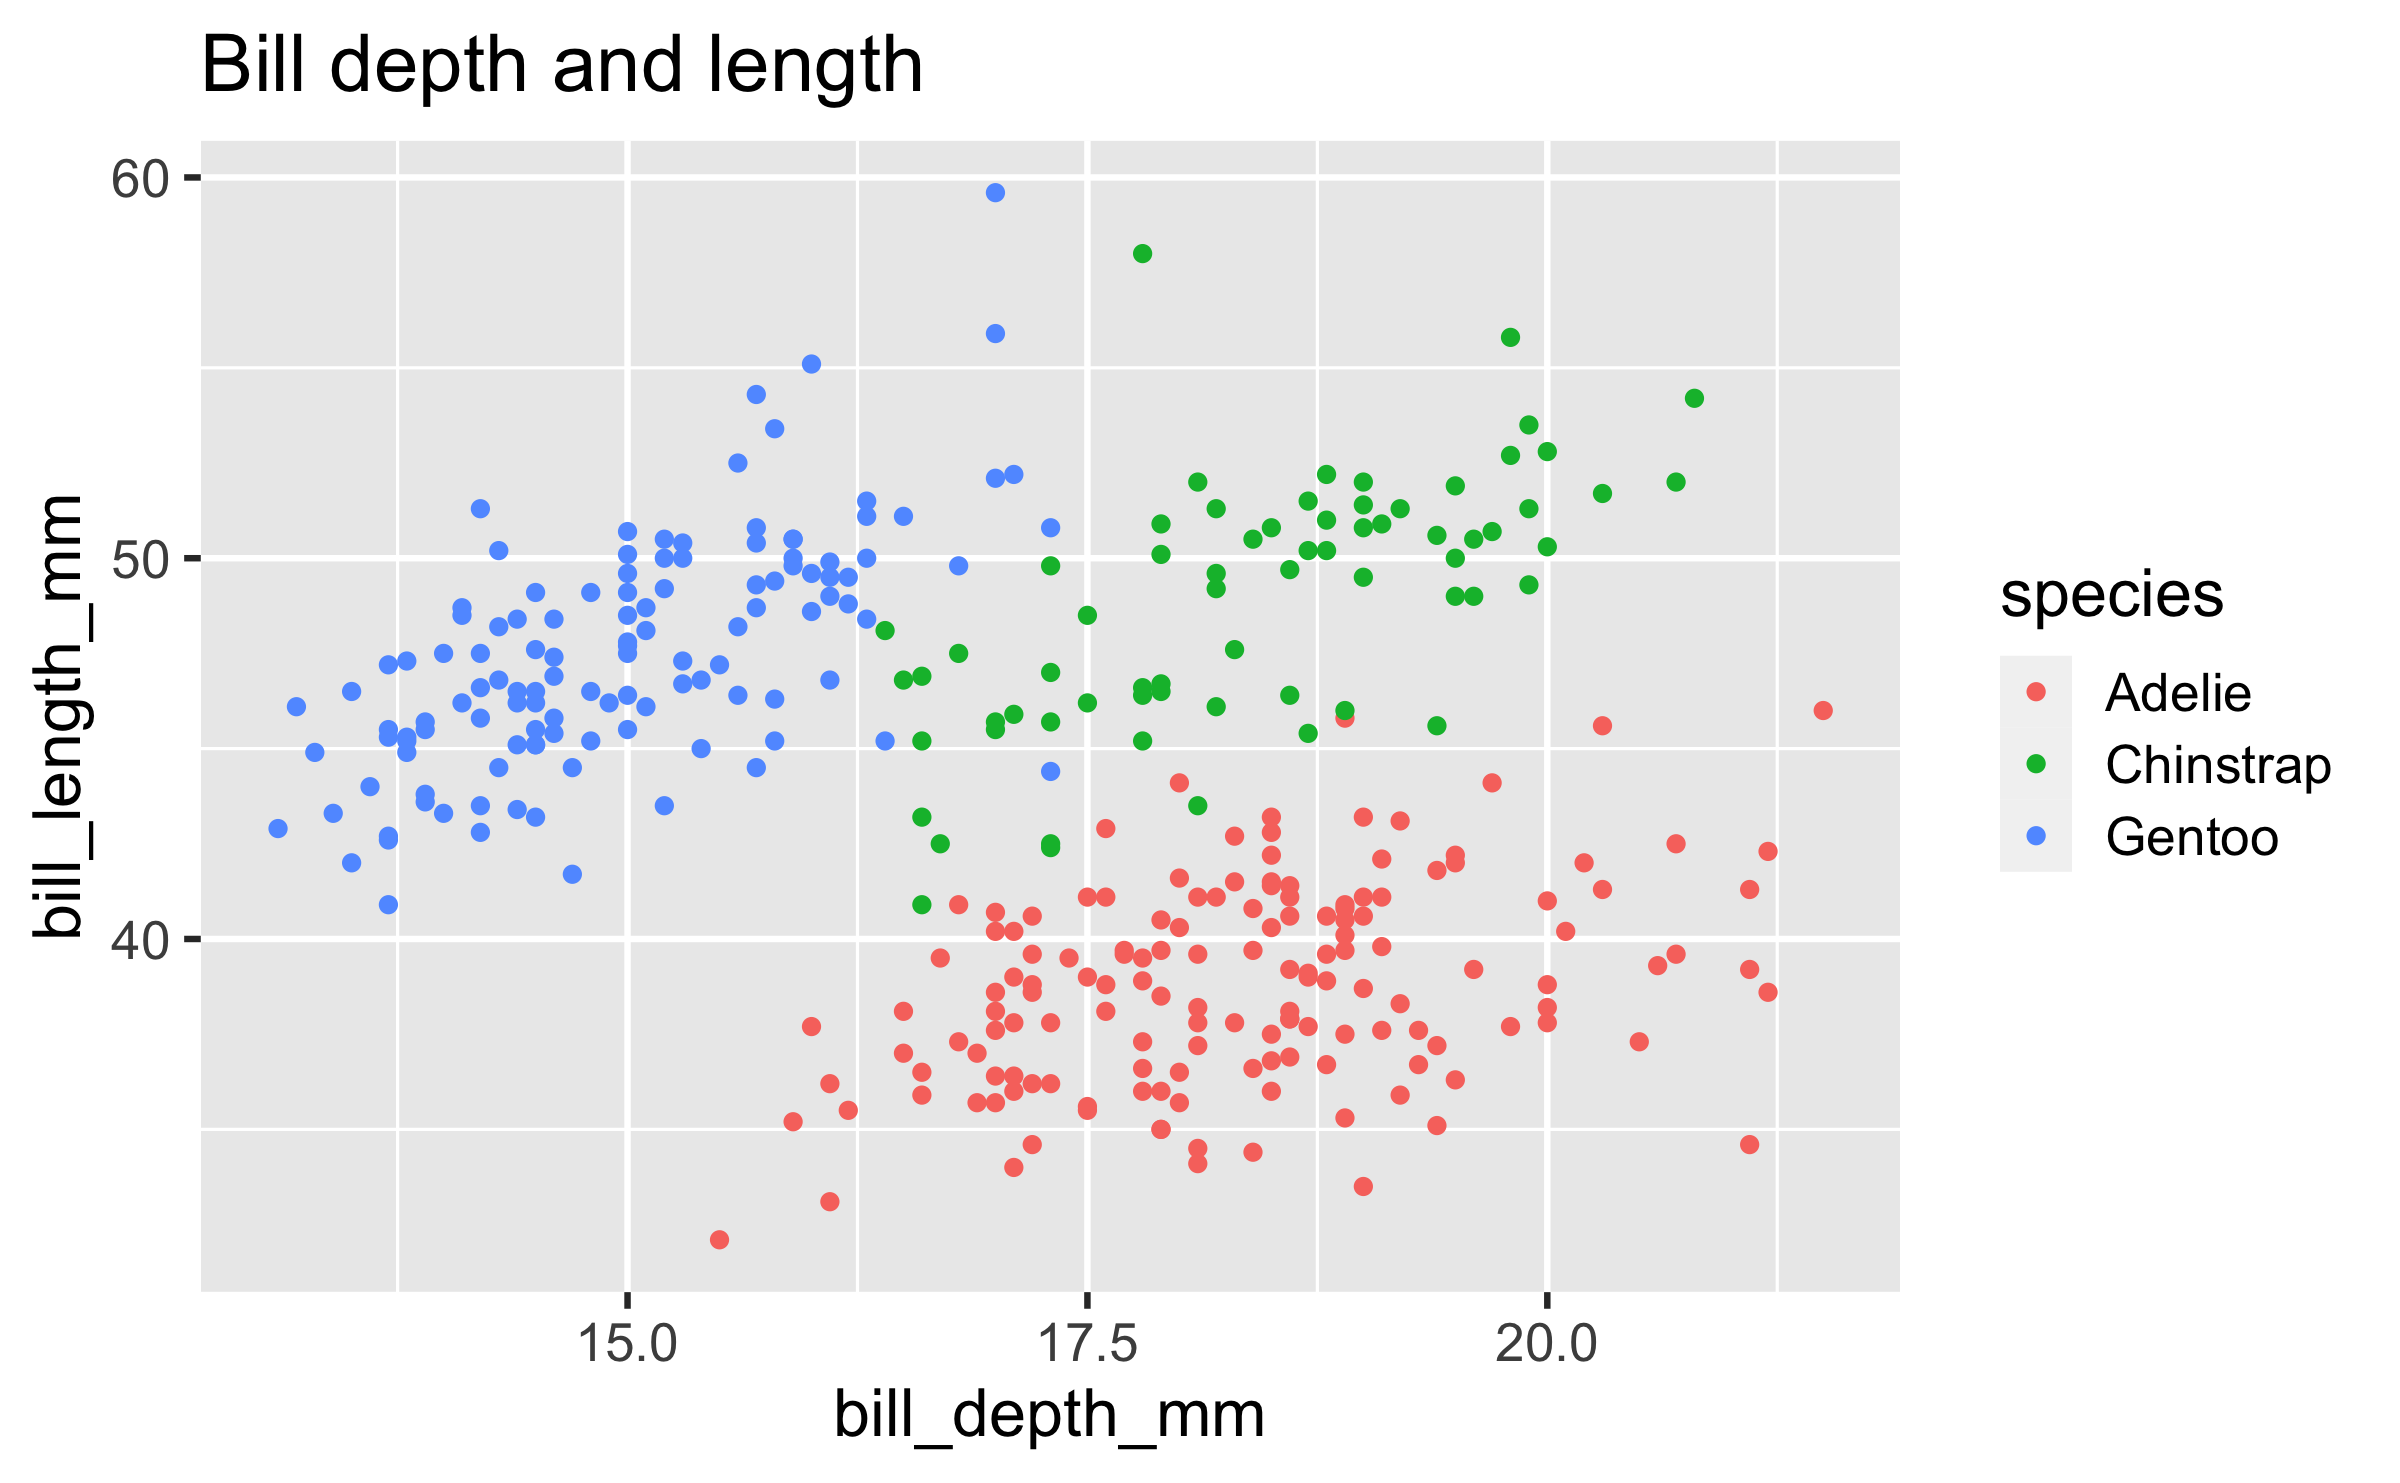
\includegraphics[width=1\linewidth]{Images/S2/penguins-5-1}
			
		\end{figure}
		
		
	\end{minipage}
	
\end{frame}
%------------------------------------------------------------------%
	\begin{frame}
	
	\small{Start with the penguins data frame, map bill depth to the x-axis and map bill length to the y-axis. Represent each observation with a point and map species to the colour of each point. Title the plot "Bill depth and length", \structure{add the subtitle "Dimensions for Adelie, Chinstrap, and Gentoo Penguins"}}
	
	\begin{minipage}[t]{0.5\linewidth}
		\begin{figure}
			\centering
			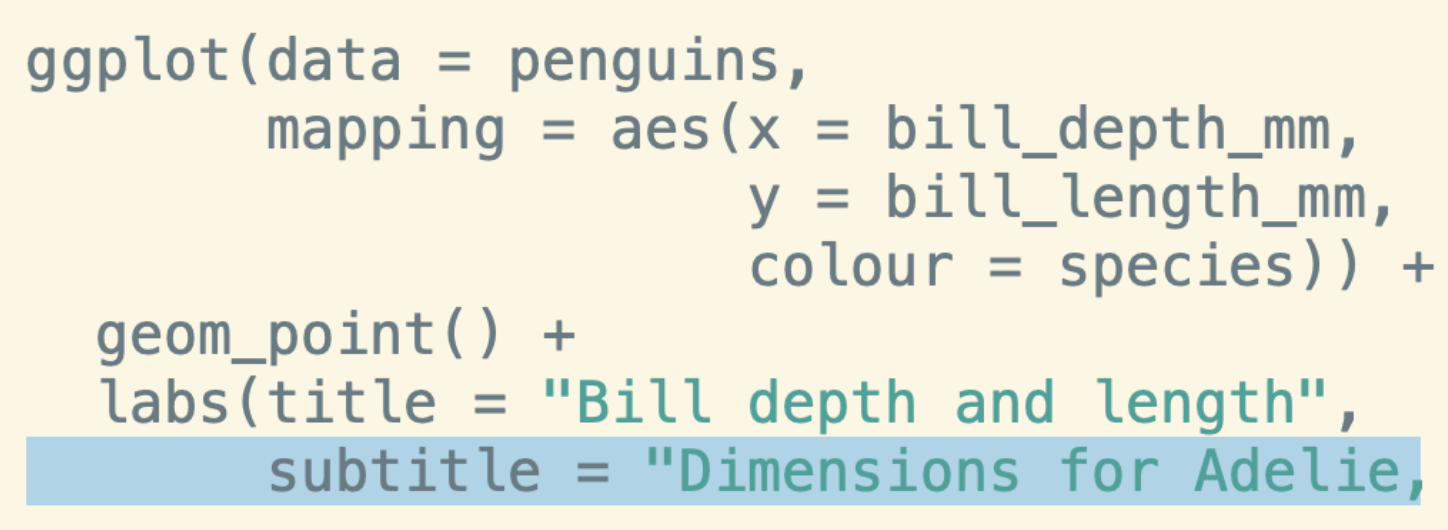
\includegraphics[width=1\linewidth]{Images/S2/code/s12}
			
		\end{figure}
	\end{minipage}%
	\begin{minipage}[t]{0.5\linewidth}
		
		\begin{figure}
			\centering
			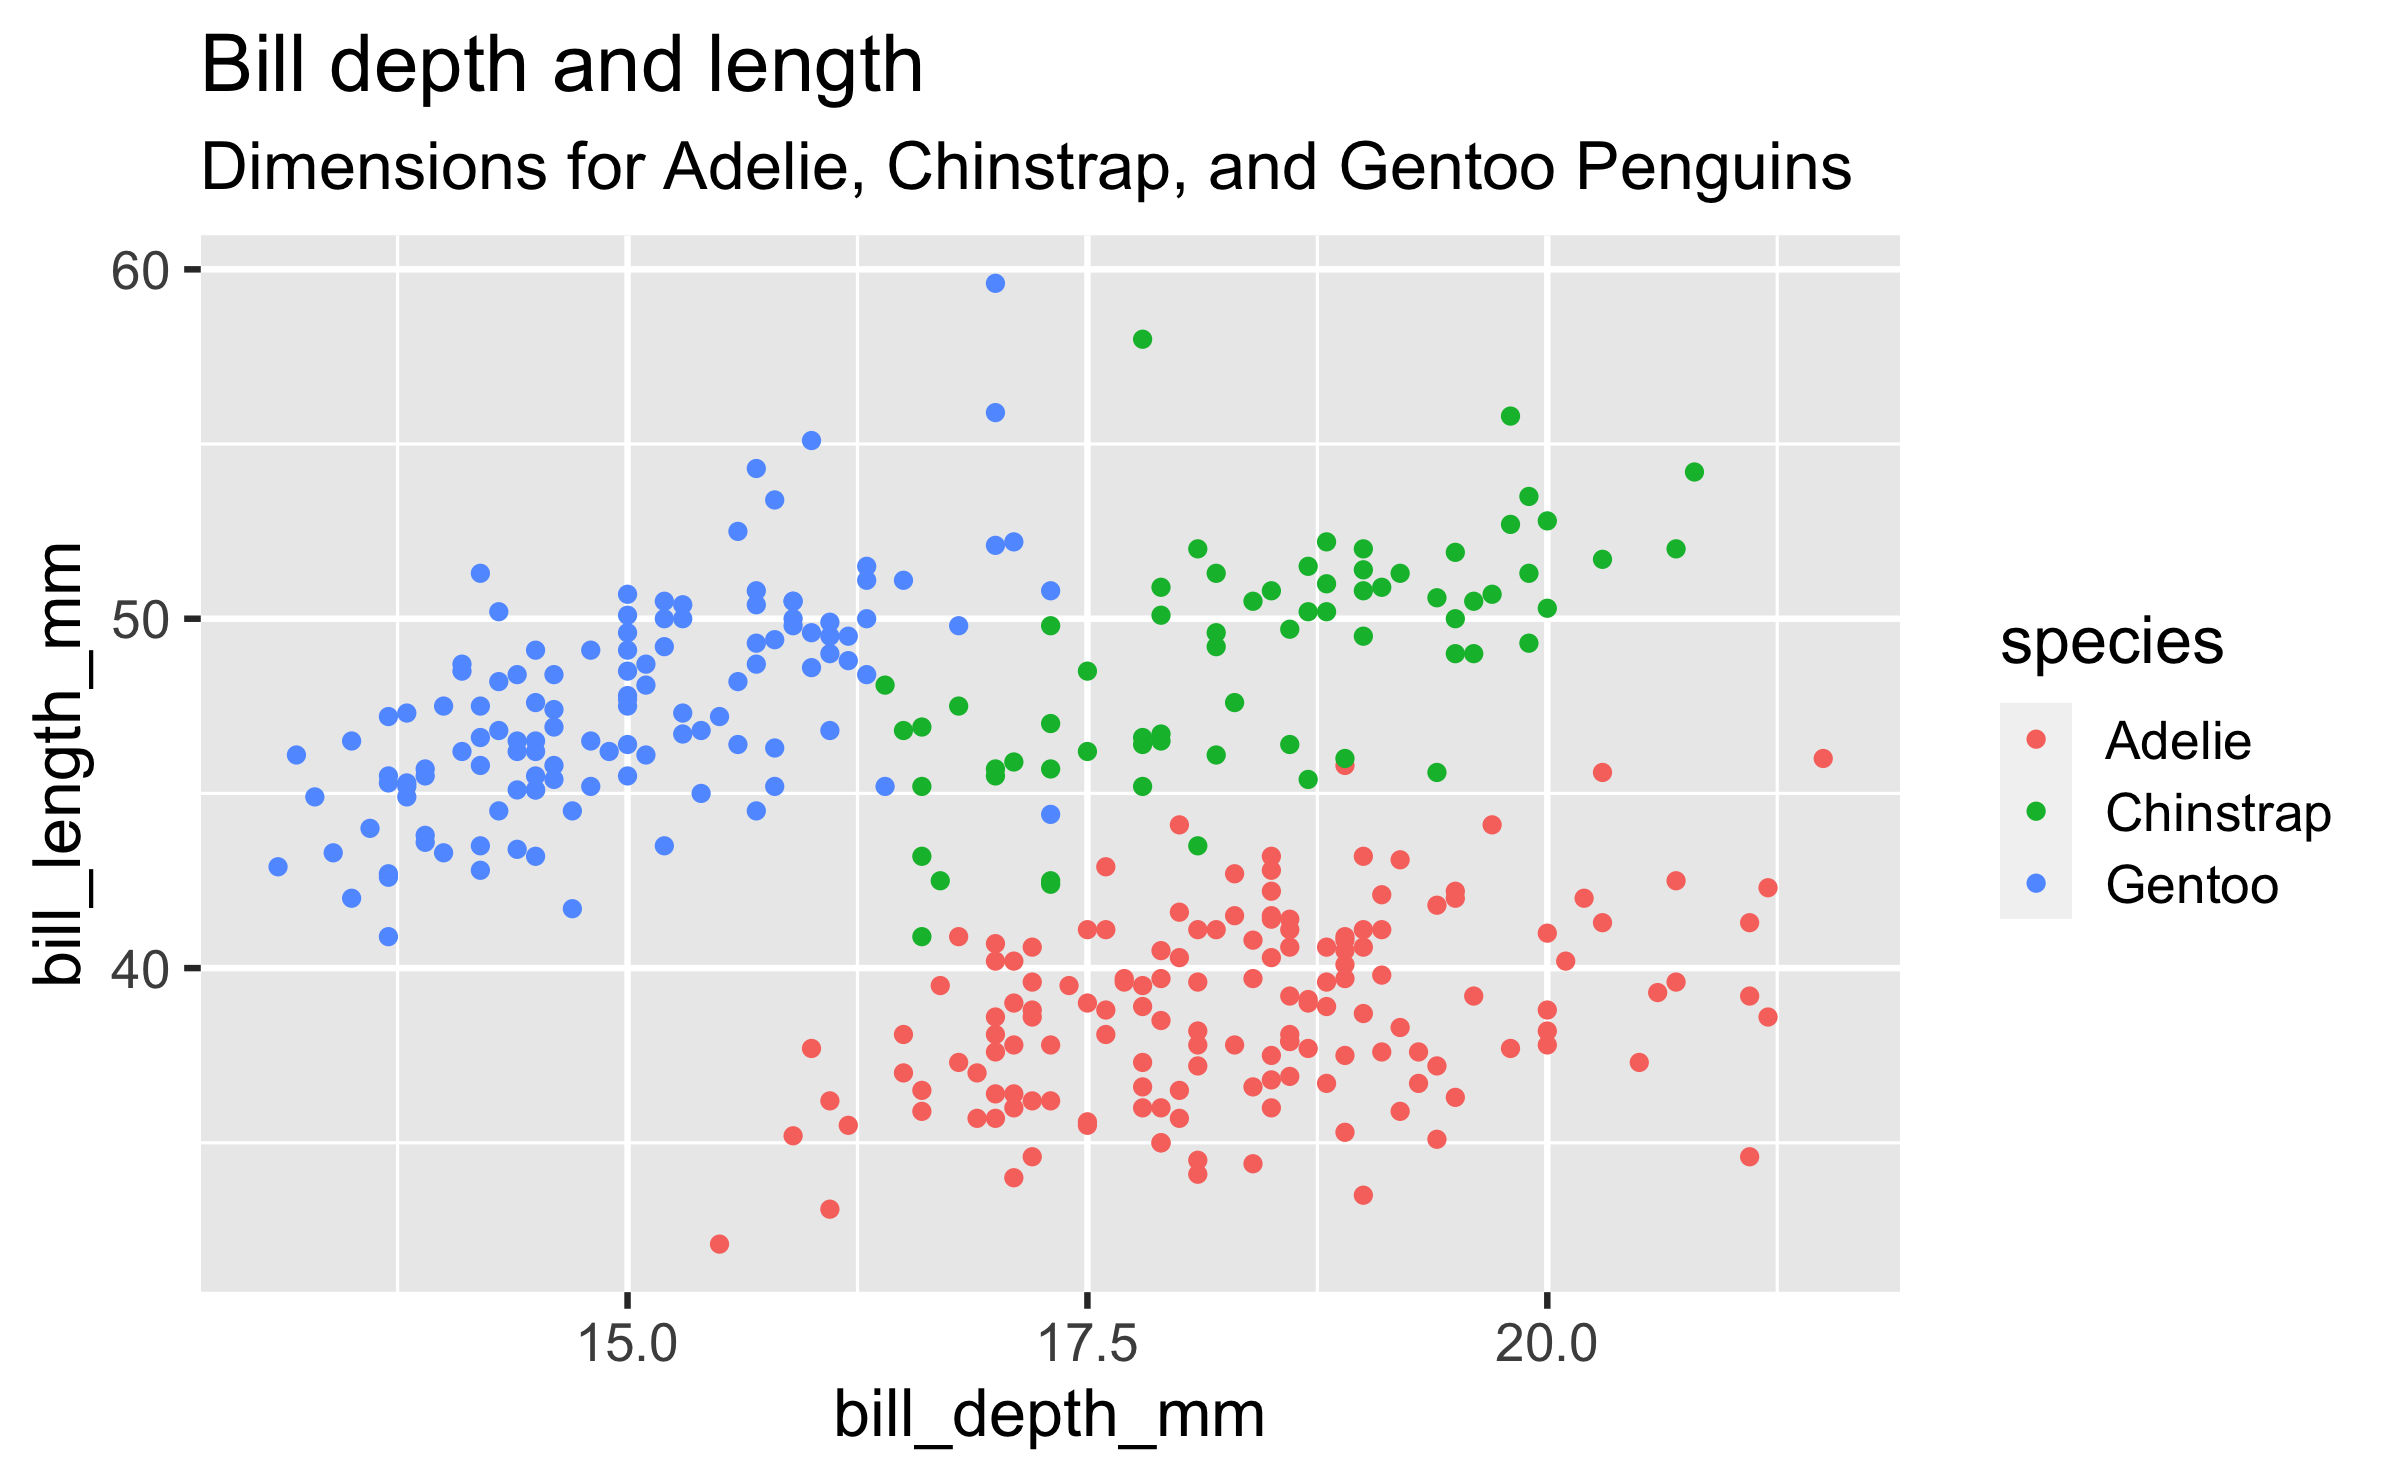
\includegraphics[width=1\linewidth]{Images/S2/penguins-6-1}
			
		\end{figure}
		
		
	\end{minipage}
	
\end{frame}
%------------------------------------------------------------------%
	\begin{frame}
	
	\small{Start with the penguins data frame, map bill depth to the x-axis and map bill length to the y-axis. Represent each observation with a point and map species to the colour of each point. Title the plot "Bill depth and length", add the subtitle "Dimensions for Adelie, Chinstrap, and Gentoo Penguins", \structure{label the x and y axes as "Bill depth (mm)" and "Bill length (mm)", respectively}}
	
	\begin{minipage}[t]{0.5\linewidth}
		\begin{figure}
			\centering
			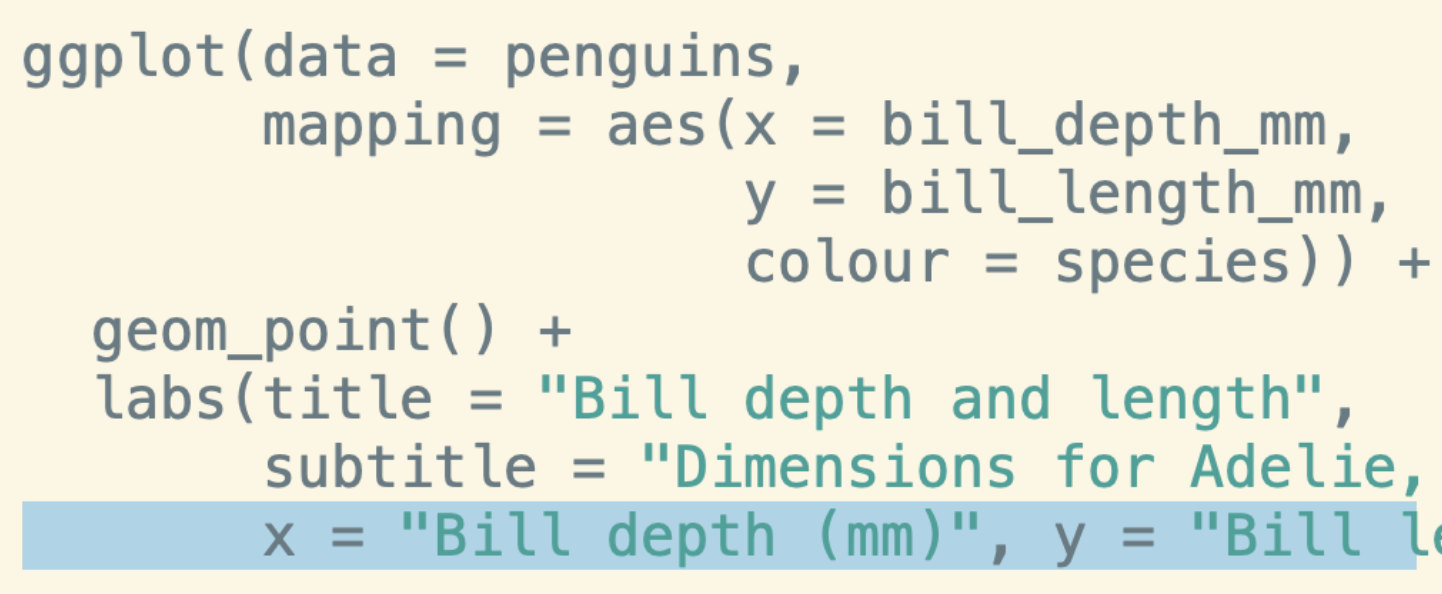
\includegraphics[width=1\linewidth]{Images/S2/code/s13}
			
		\end{figure}
	\end{minipage}%
	\begin{minipage}[t]{0.5\linewidth}
		
		\begin{figure}
			\centering
			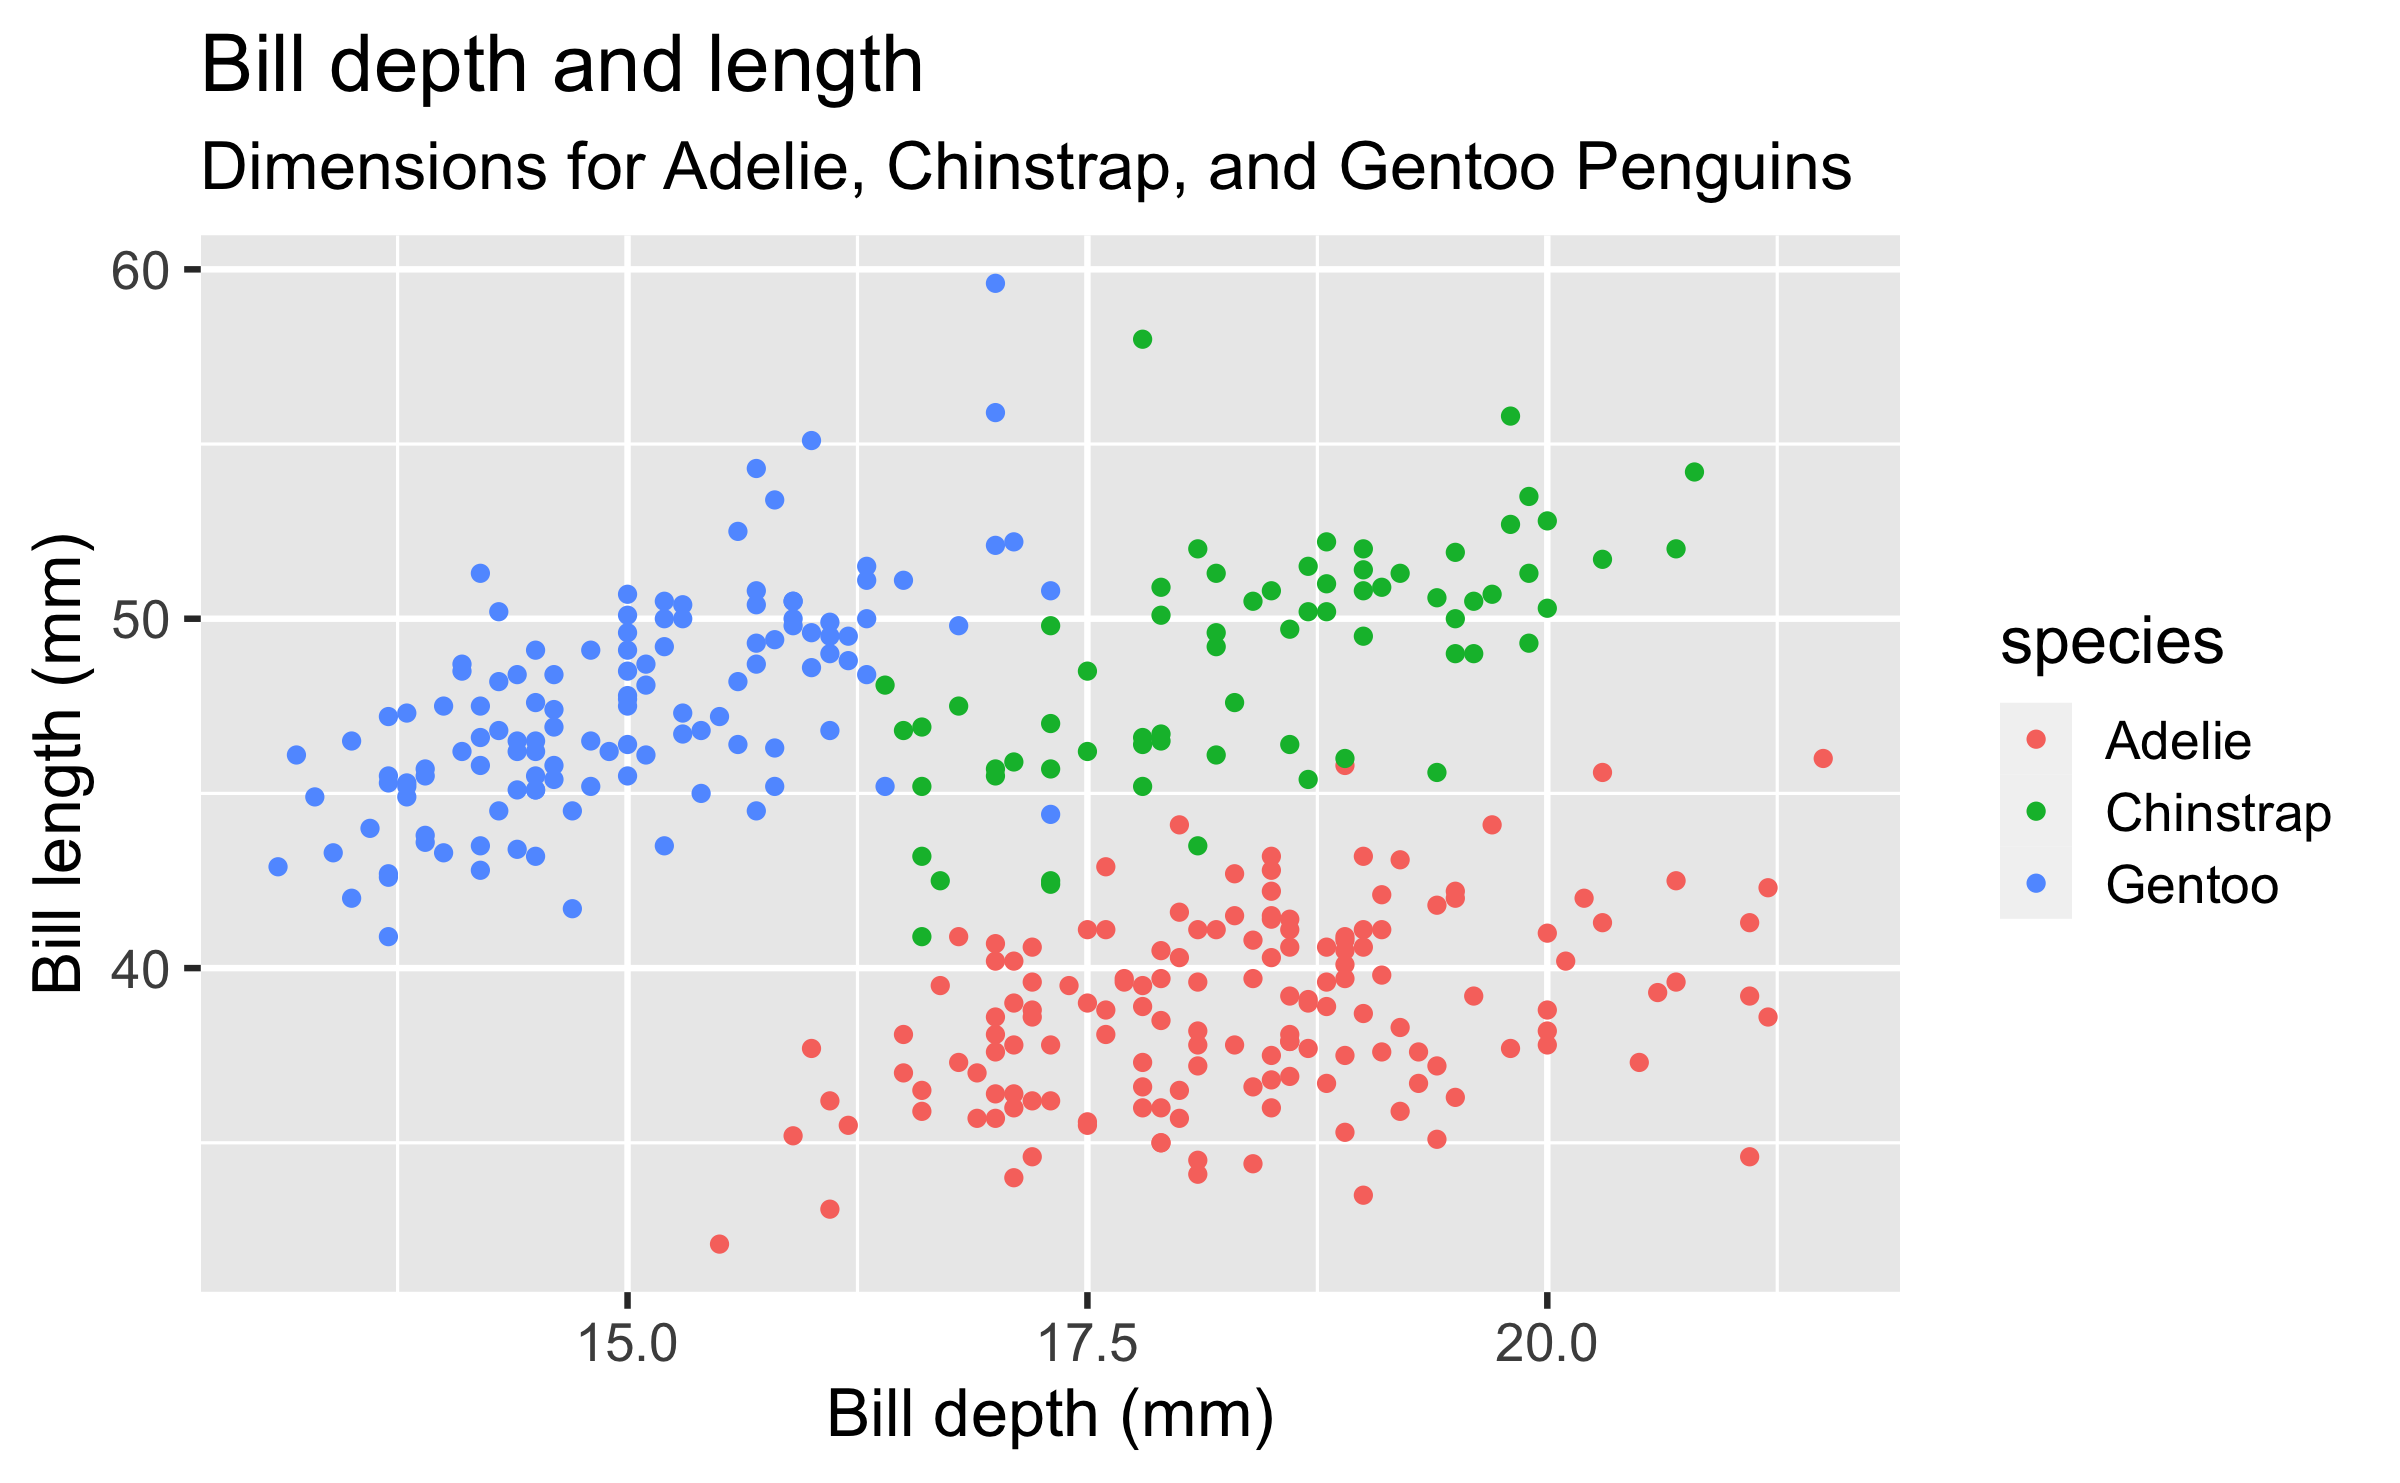
\includegraphics[width=1\linewidth]{Images/S2/penguins-7-1}
			
		\end{figure}
		
		
	\end{minipage}
	
\end{frame}
%------------------------------------------------------------------%
	\begin{frame}
	
	\small{Start with the penguins data frame, map bill depth to the x-axis and map bill length to the y-axis. Represent each observation with a point and map species to the colour of each point. Title the plot "Bill depth and length", add the subtitle "Dimensions for Adelie, Chinstrap, and Gentoo Penguins", label the x and y axes as "Bill depth (mm)" and "Bill length (mm)", respectively, \structure{label the legend "Species"}}
	
	\begin{minipage}[t]{0.5\linewidth}
		\begin{figure}
			\centering
			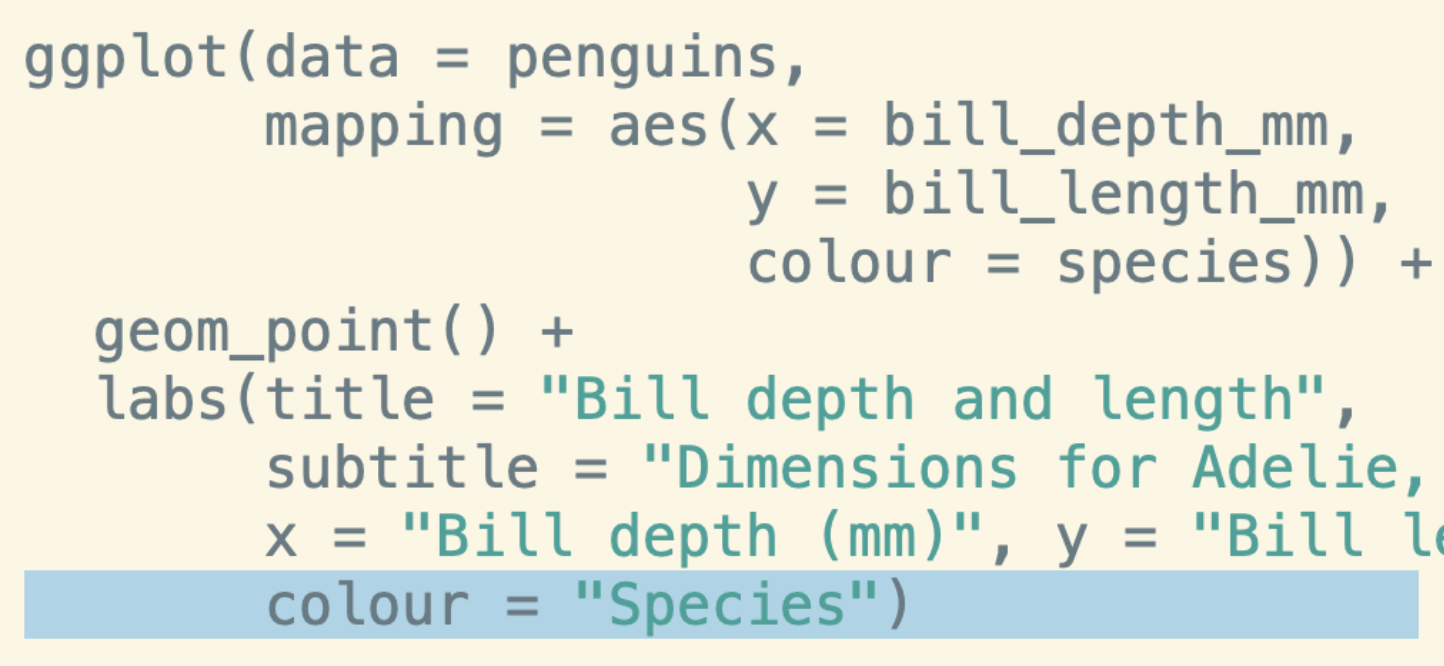
\includegraphics[width=1\linewidth]{Images/S2/code/s14}
			
		\end{figure}
	\end{minipage}%
	\begin{minipage}[t]{0.5\linewidth}
		
		\begin{figure}
			\centering
			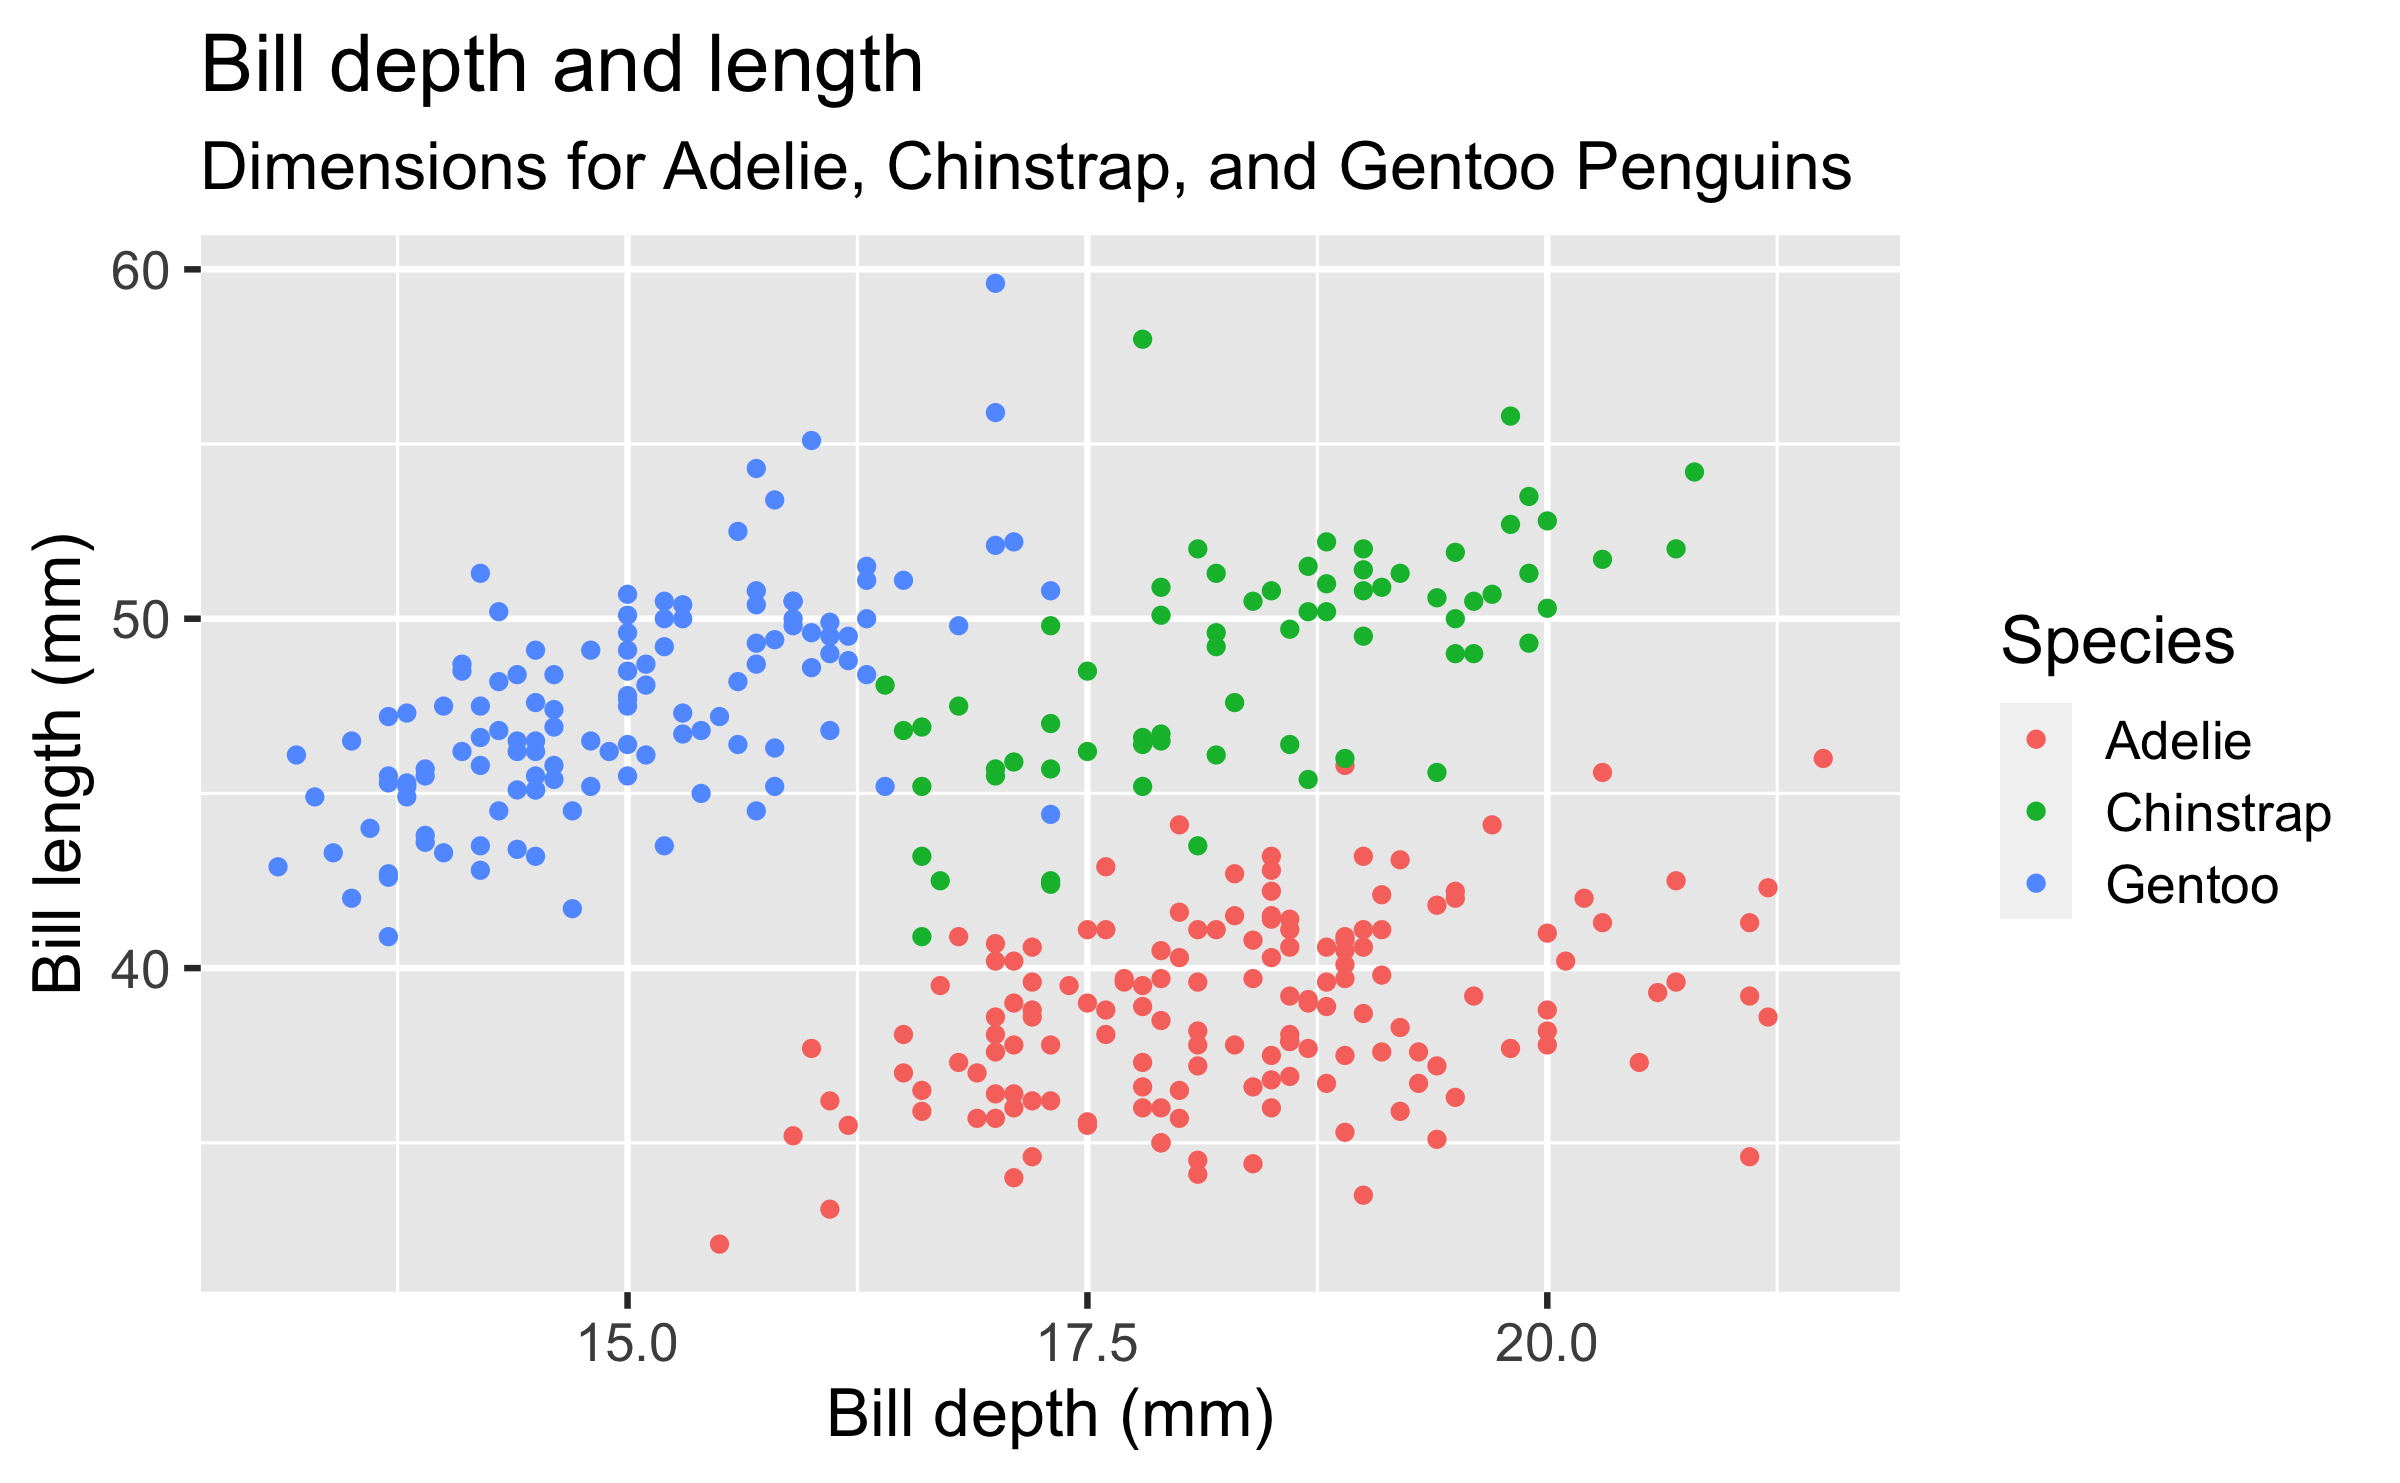
\includegraphics[width=1\linewidth]{Images/S2/penguins-8-1}
			
		\end{figure}
		
		
	\end{minipage}
	
\end{frame}
%------------------------------------------------------------------%
	\begin{frame}
	
	\small{Start with the penguins data frame, map bill depth to the x-axis and map bill length to the y-axis. Represent each observation with a point and map species to the colour of each point. Title the plot "Bill depth and length", add the subtitle "Dimensions for Adelie, Chinstrap, and Gentoo Penguins", label the x and y axes as "Bill depth (mm)" and "Bill length (mm)", respectively, label the legend "Species", \structure{and add a caption for the data source.}}
	
	\begin{minipage}[t]{0.5\linewidth}
		\begin{figure}
			\centering
			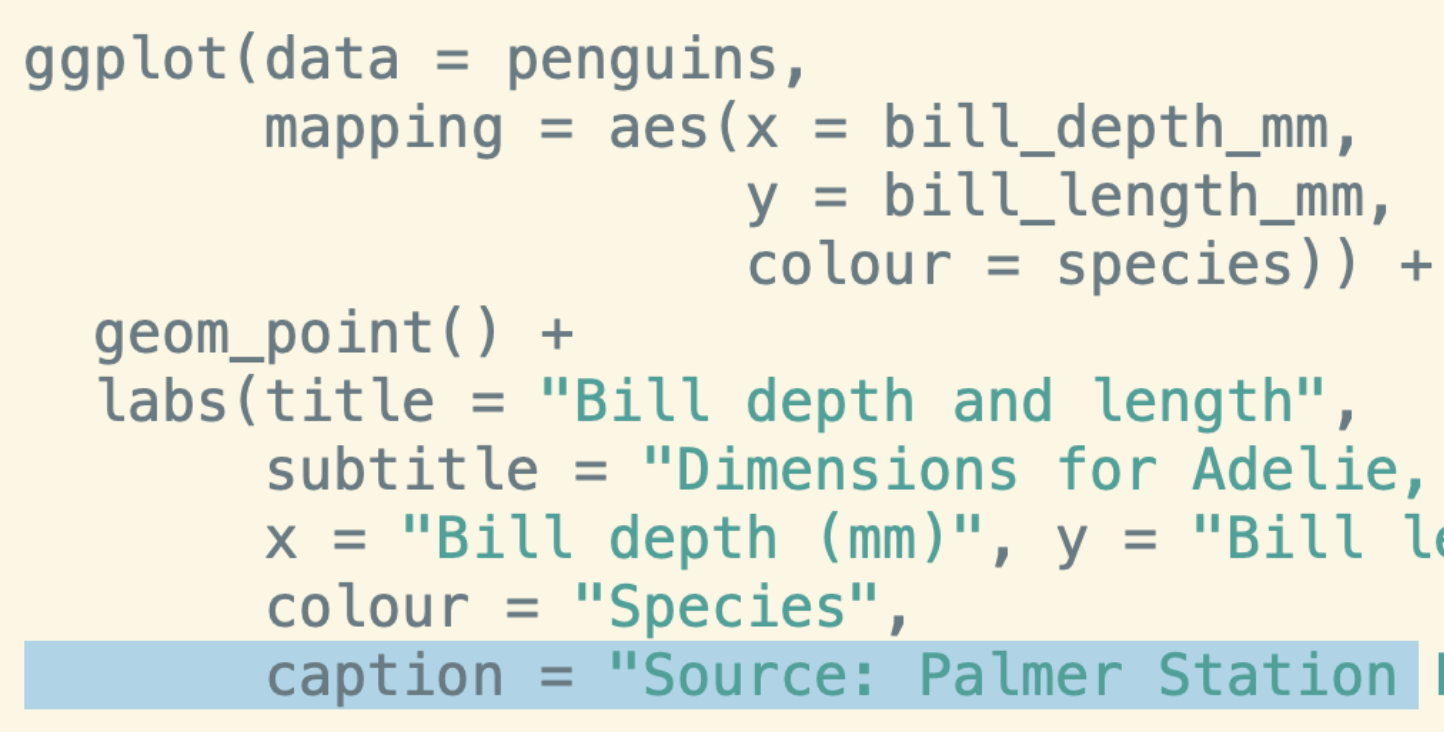
\includegraphics[width=1\linewidth]{Images/S2/code/s15}
			
		\end{figure}
	\end{minipage}%
	\begin{minipage}[t]{0.5\linewidth}
		
		\begin{figure}
			\centering
			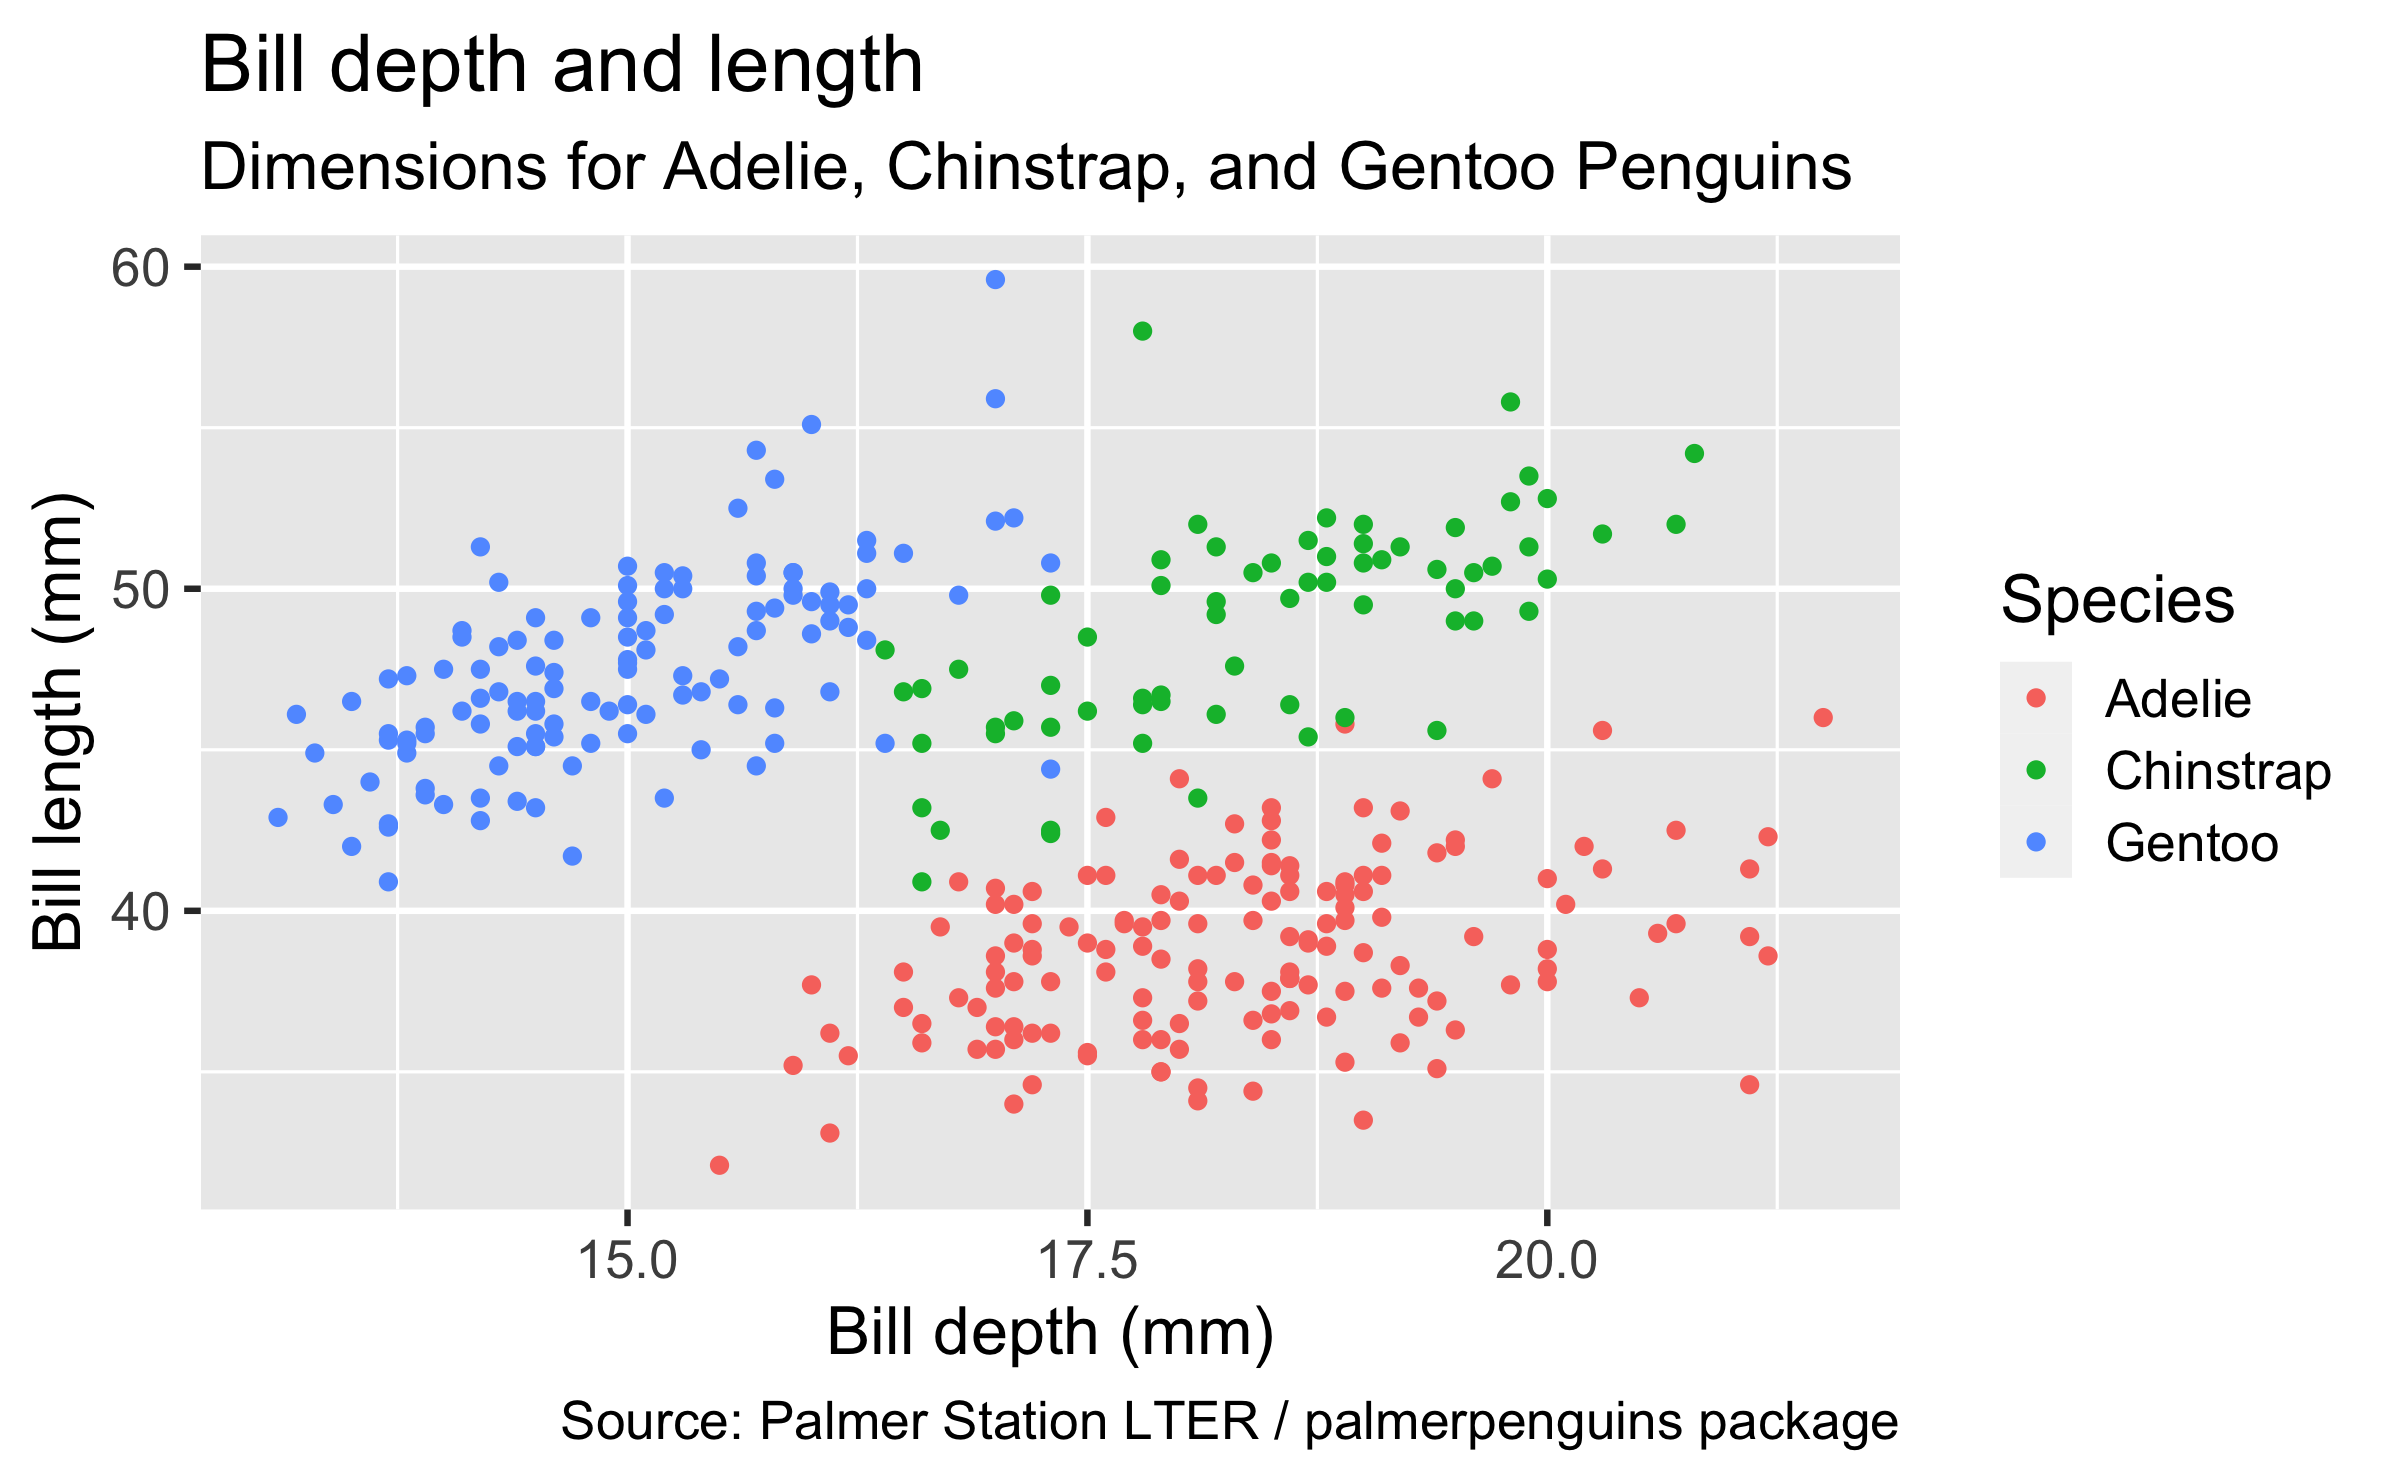
\includegraphics[width=1\linewidth]{Images/S2/penguins-9-1}
			
		\end{figure}
		
		
	\end{minipage}
	
\end{frame}
%------------------------------------------------------------------%
	\begin{frame}
	
	\small{Start with the penguins data frame, map bill depth to the x-axis and map bill length to the y-axis. Represent each observation with a point and map species to the colour of each point. Title the plot "Bill depth and length", add the subtitle "Dimensions for Adelie, Chinstrap, and Gentoo Penguins", label the x and y axes as "Bill depth (mm)" and "Bill length (mm)", respectively, label the legend "Species", and add a caption for the data source. \structure{Finally, use a discrete colour scale that is designed to be perceived by viewers with common forms of colour blindness.}}
	\vspace{-1.5em}
	
	\begin{minipage}[t]{0.5\linewidth}
		\begin{figure}
			\centering
			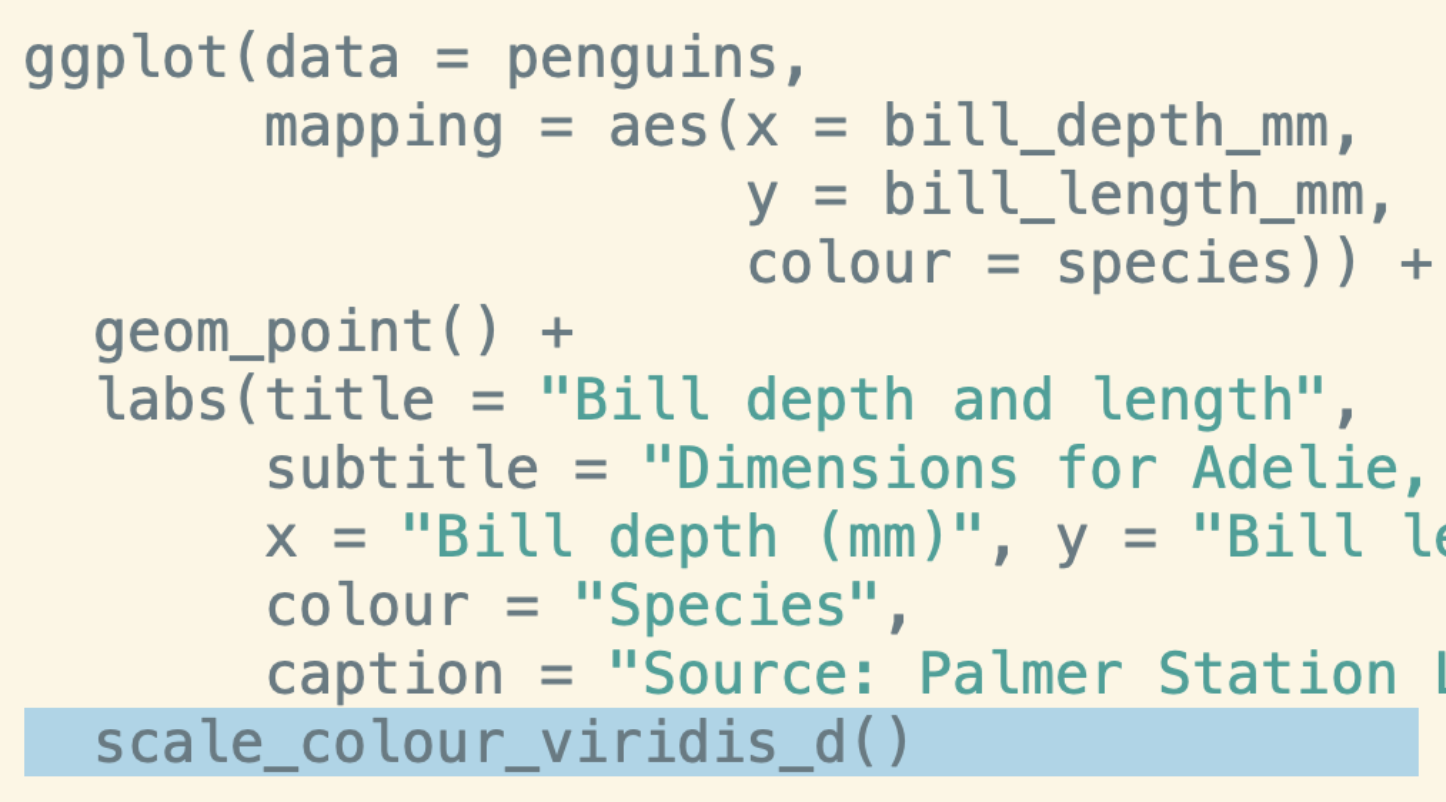
\includegraphics[width=1\linewidth]{Images/S2/code/s16}
			
		\end{figure}
	\end{minipage}%
	\begin{minipage}[t]{0.5\linewidth}
		
		\begin{figure}
			\centering
			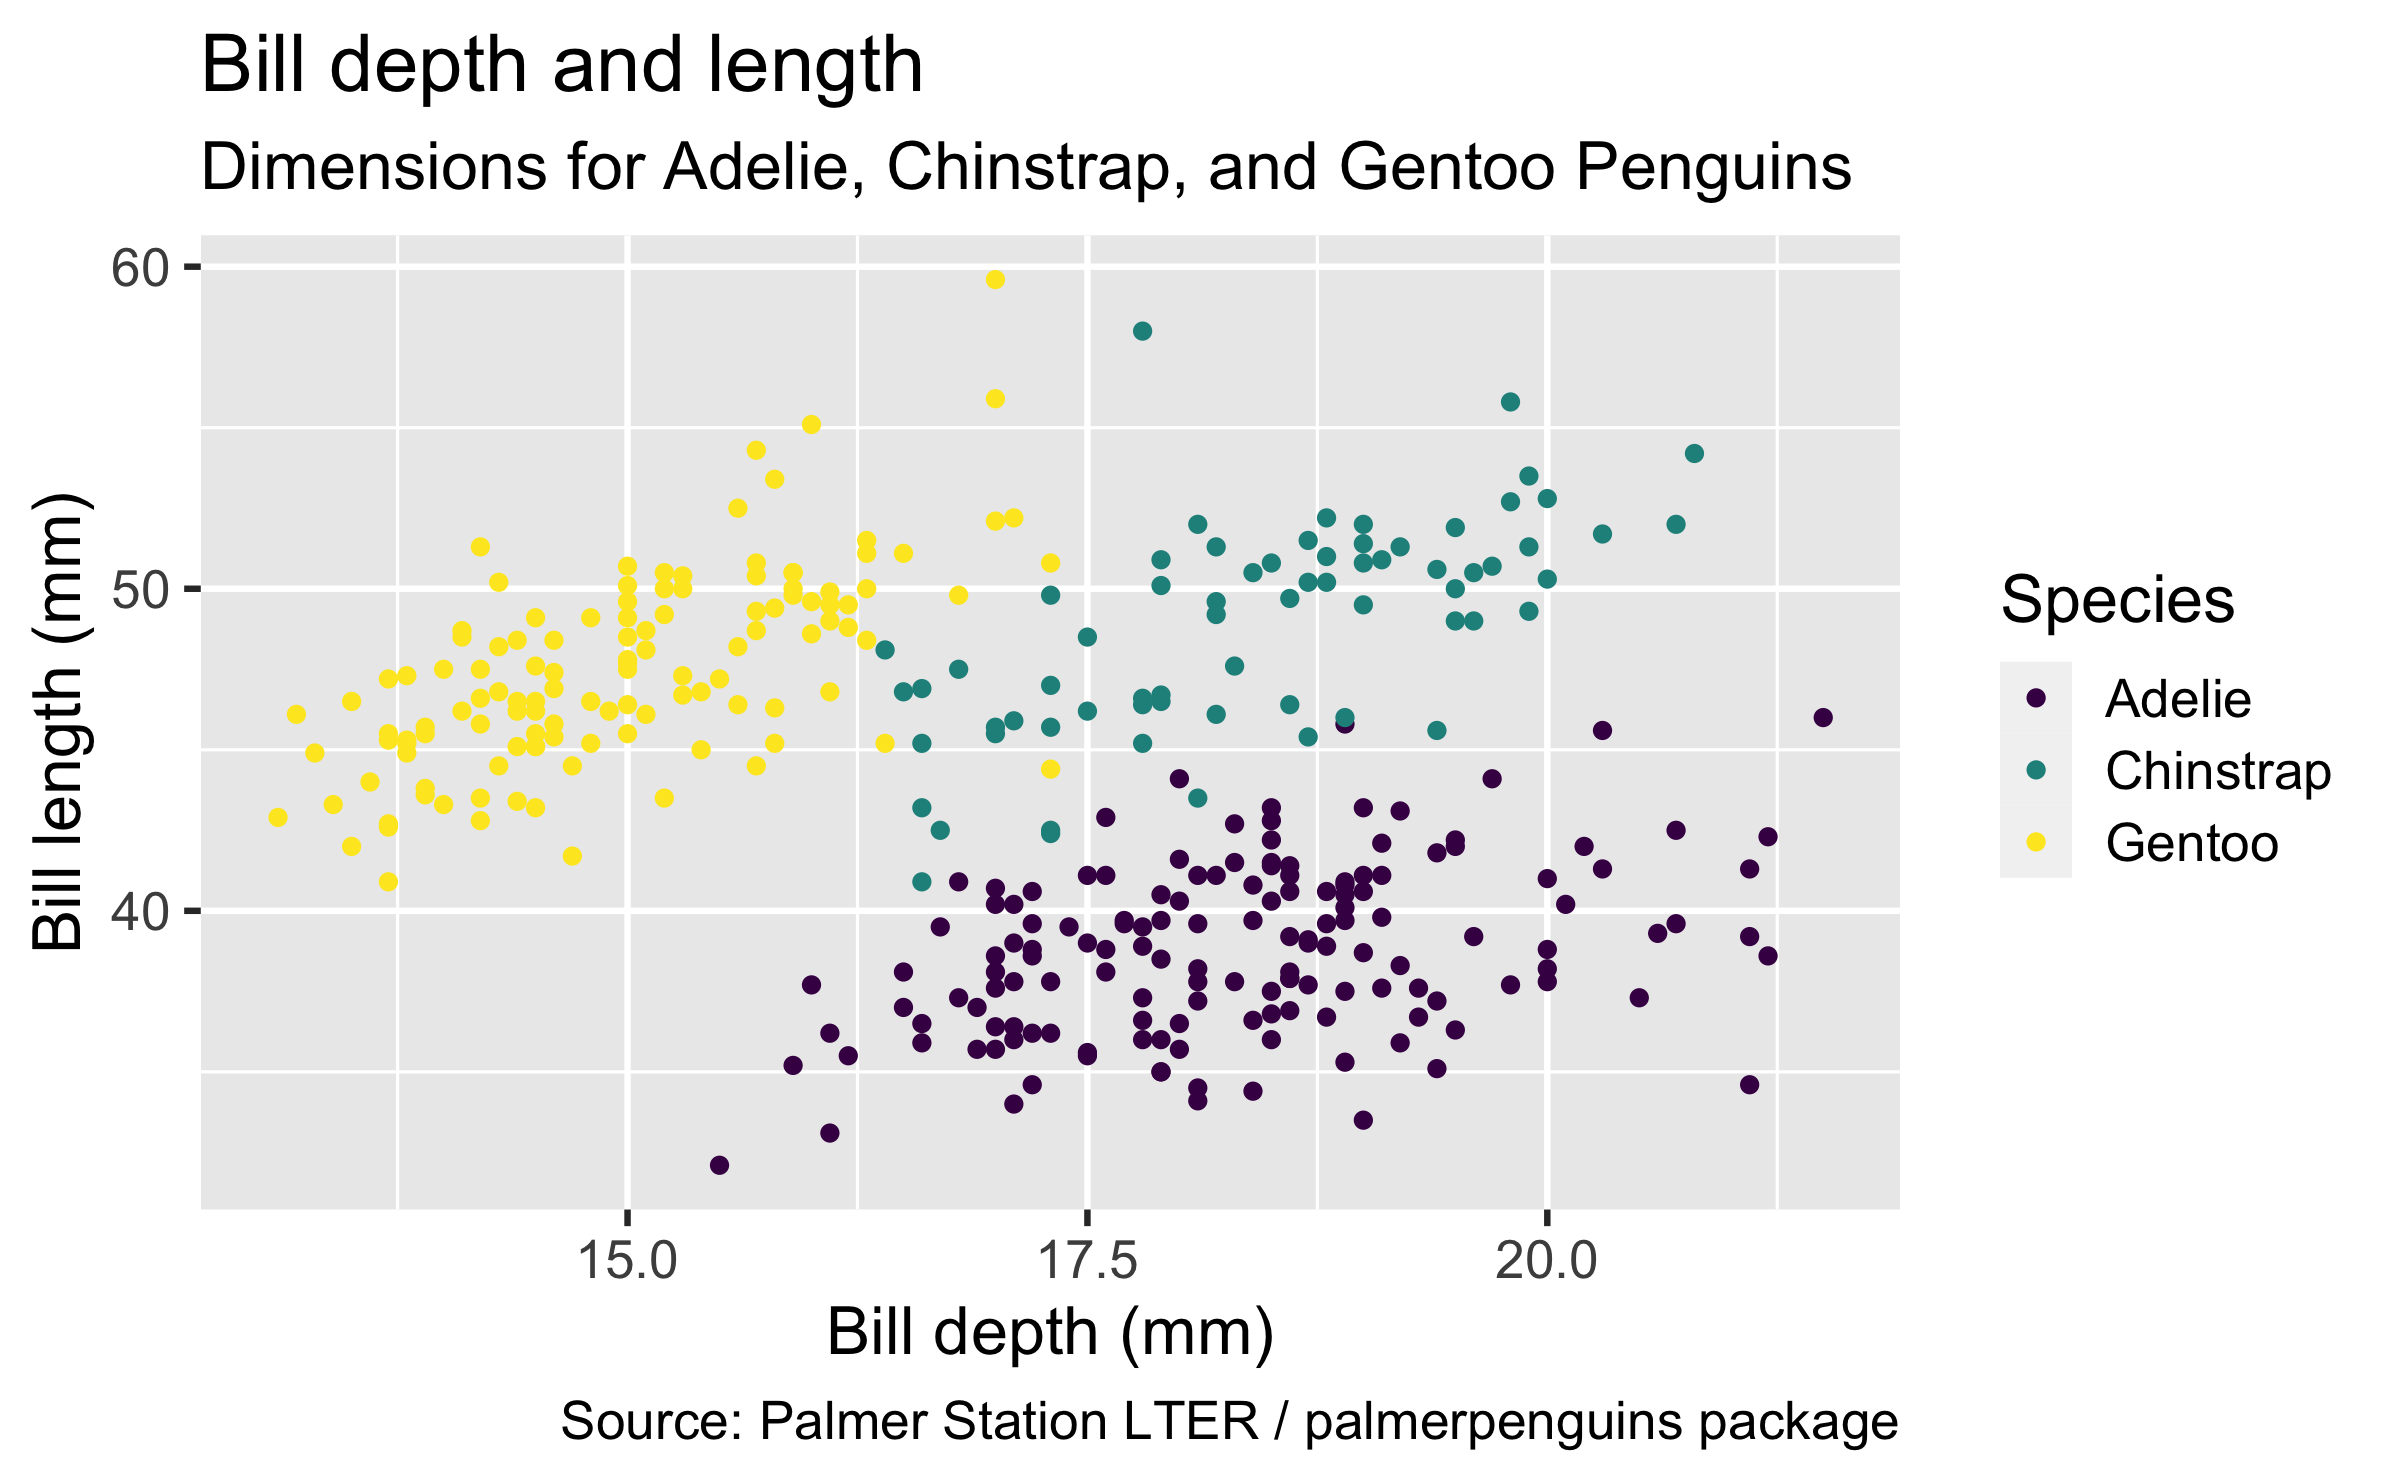
\includegraphics[width=1\linewidth]{Images/S2/penguins-10-1}
			
		\end{figure}
		
		
	\end{minipage}
	
\end{frame}
%------------------------------------------------------------------%
	\begin{frame}
	\frametitle{\textbf{Argument Names}}
		\begin{figure}
			\centering
			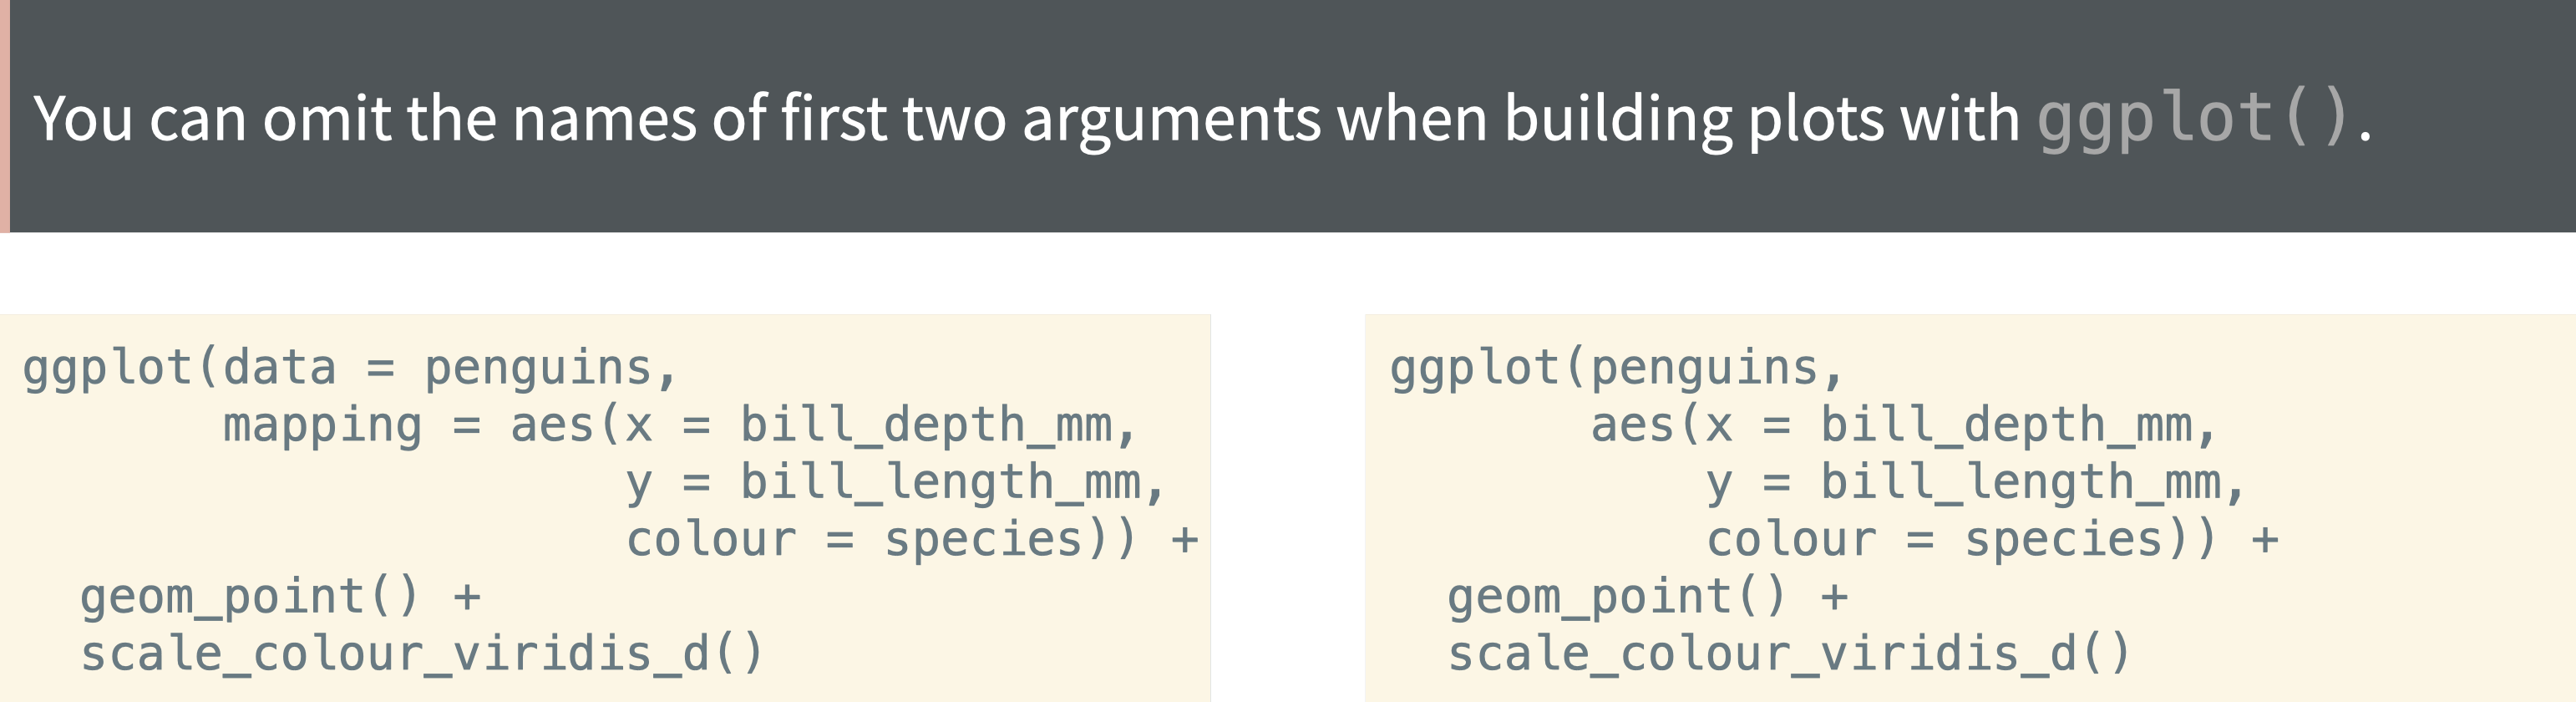
\includegraphics[width=1\linewidth]{Images/S2/code/s17}
			
		\end{figure}
	
\end{frame}
%------------------------------------------------------------------%
%------------------------------------------------------------------%
\begin{frame}
	\frametitle{\textbf{Aesthetics Options}}
	Commonly used characteristics of plotting characters that can be \textit{mapped to a specific variable} in the data are
	
\begin{itemize}
	\item colour
	\item shape
	\item size
	\item alpha (transparency)
\end{itemize}
	
\end{frame}
%------------------------------------------------------------------%

\begin{frame}
	\frametitle{\textbf{Colour}}

		\begin{minipage}[t]{0.5\linewidth}
			\begin{figure}
				\centering
				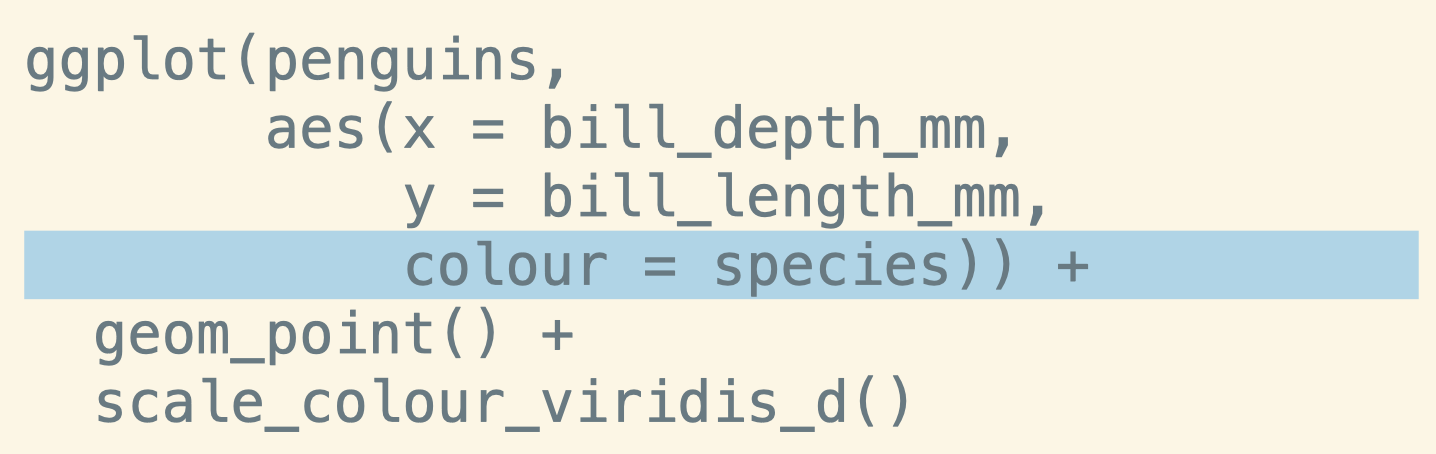
\includegraphics[width=1\linewidth]{Images/S2/code/s18}
				
			\end{figure}
		\end{minipage}%
		\begin{minipage}[t]{0.5\linewidth}
			
			\begin{figure}
				\centering
				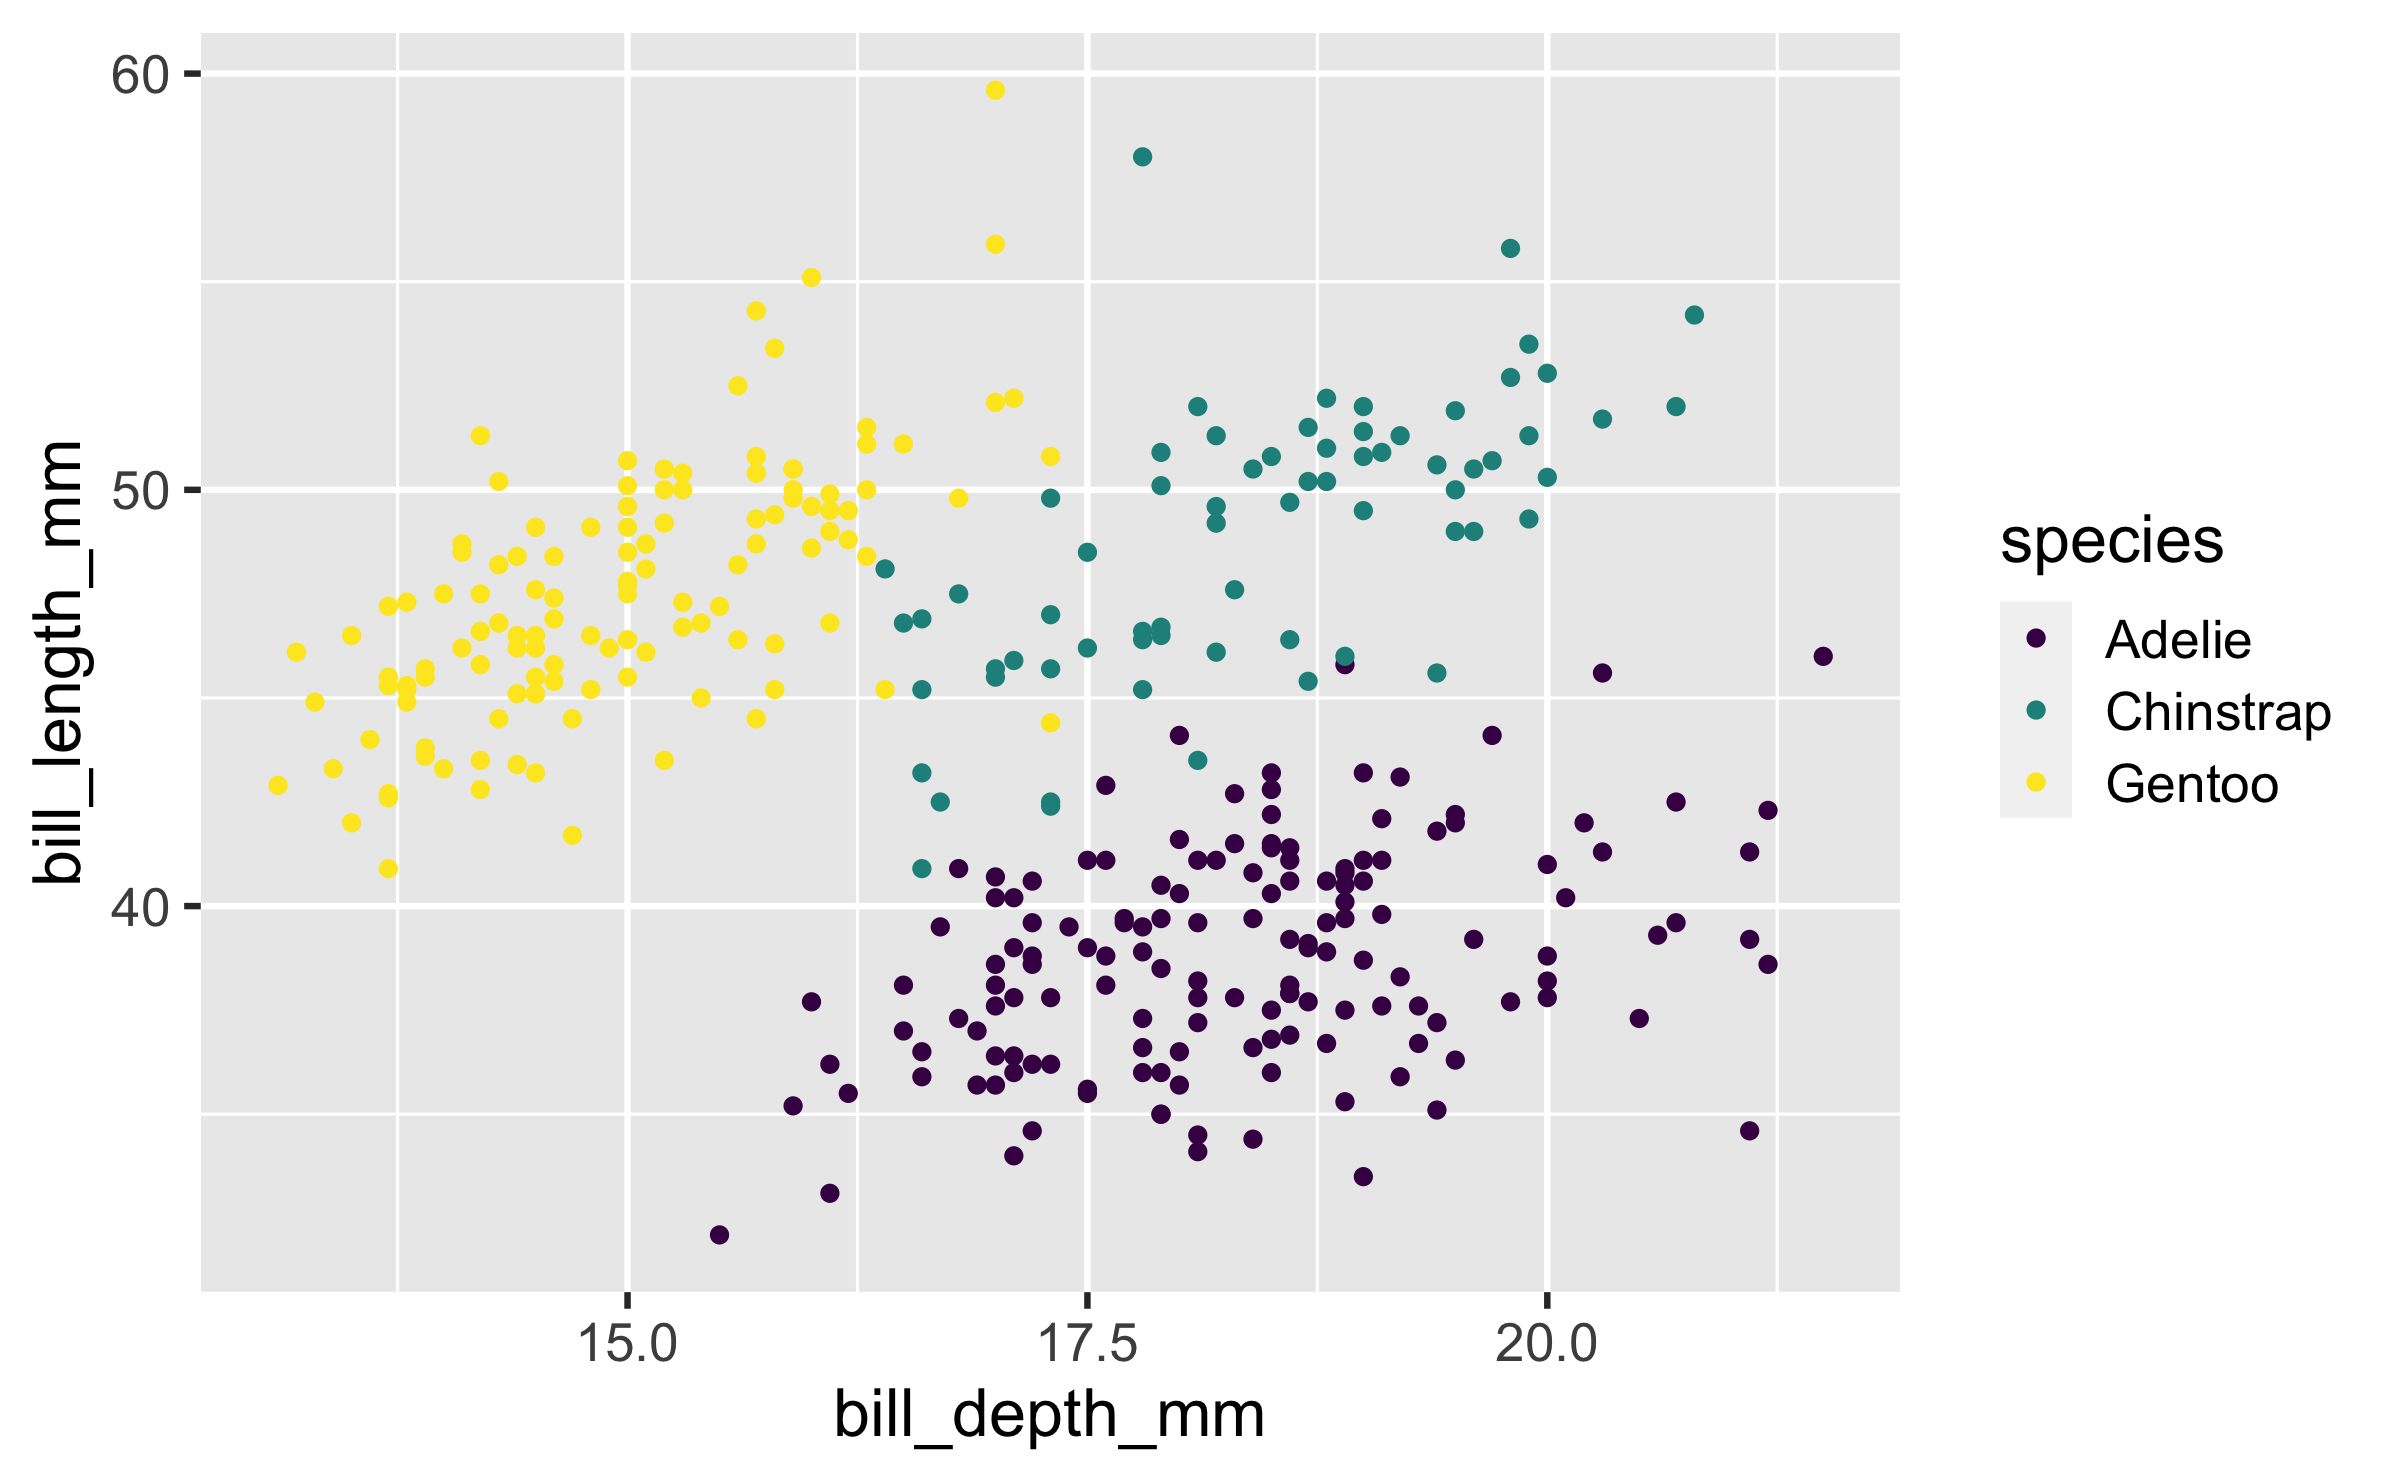
\includegraphics[width=1\linewidth]{Images/S2/colour-1}
				
			\end{figure}
			
			
		\end{minipage}
		
	
\end{frame}
%------------------------------------------------------------------%


\begin{frame}
	\frametitle{\textbf{Shape}}
	Mapped to a different variable than colour
	
	\begin{minipage}[t]{0.5\linewidth}
		\begin{figure}
			\centering
			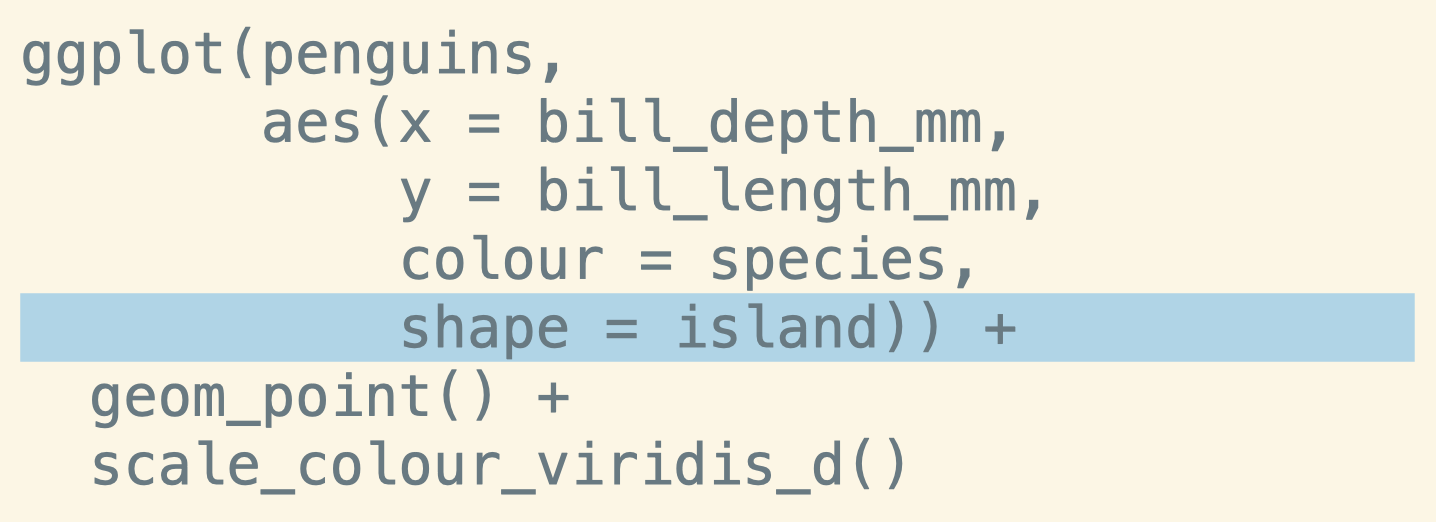
\includegraphics[width=1\linewidth]{Images/S2/code/s19}
			
		\end{figure}
	\end{minipage}%
	\begin{minipage}[t]{0.5\linewidth}
		
		\begin{figure}
			\centering
			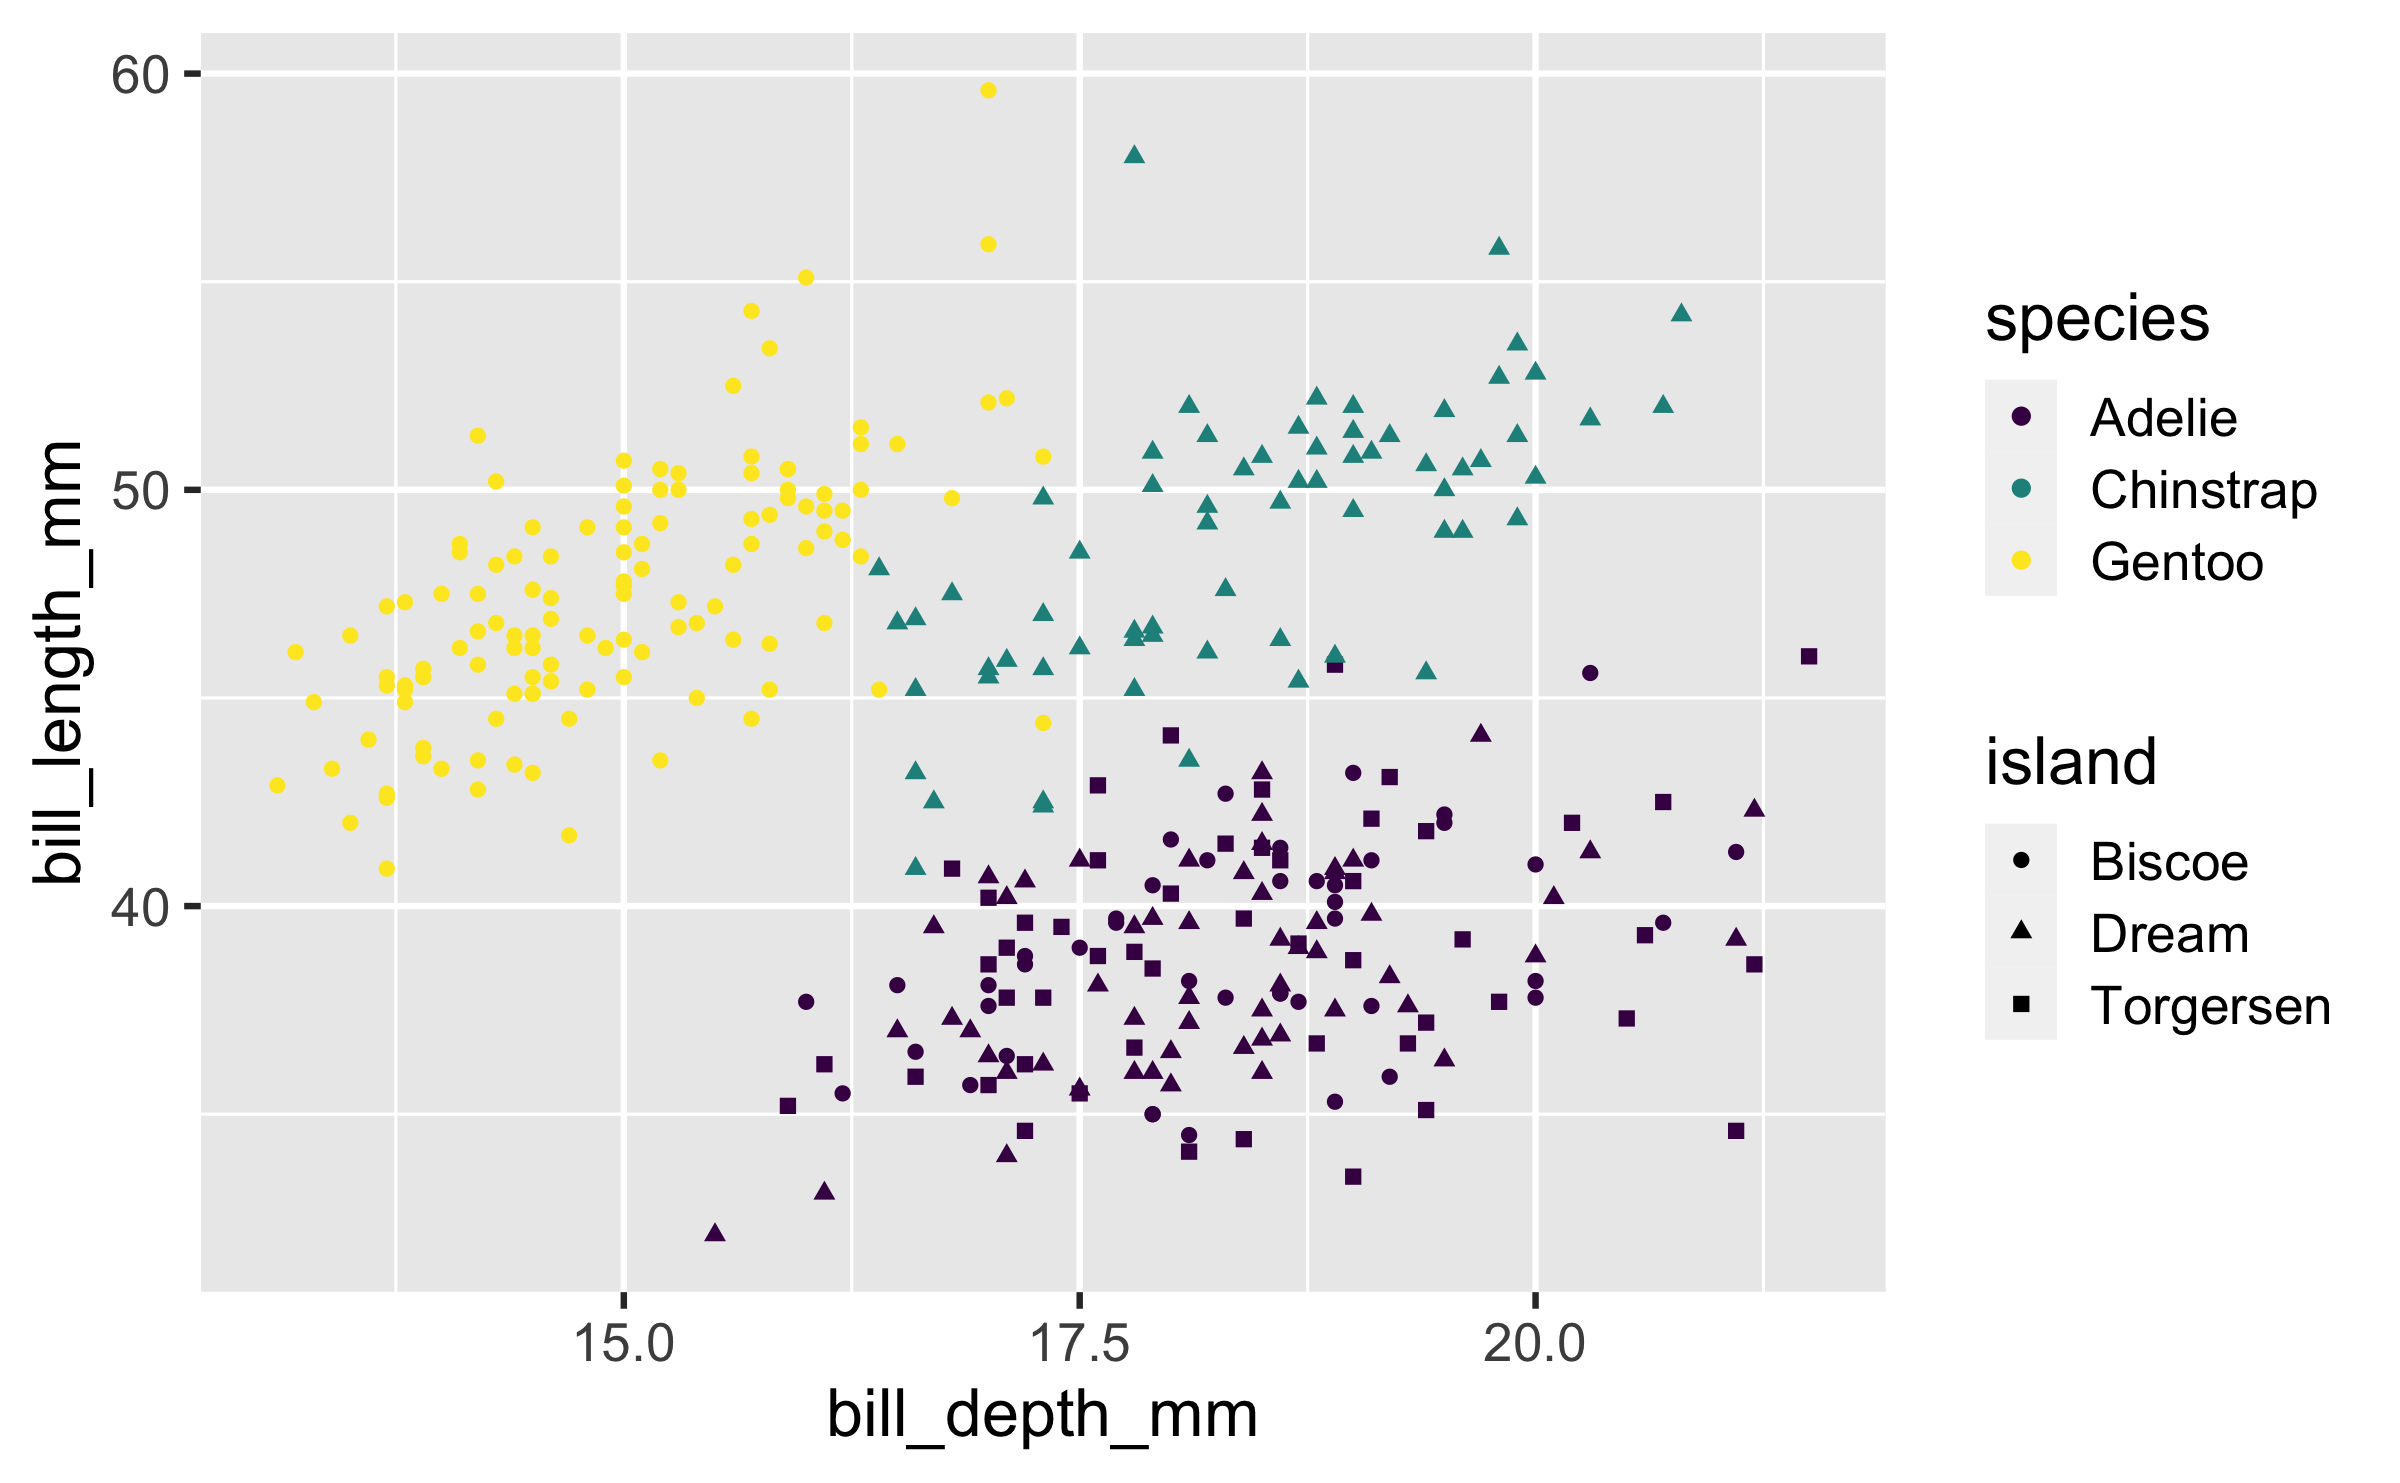
\includegraphics[width=1\linewidth]{Images/S2/shape-island-1}
			
		\end{figure}
		
		
	\end{minipage}
	
	
\end{frame}
%------------------------------------------------------------------%

\begin{frame}
	\frametitle{\textbf{Size}}
	Mapped to a different variable than colour
	
	\begin{minipage}[t]{0.5\linewidth}
		\begin{figure}
			\centering
			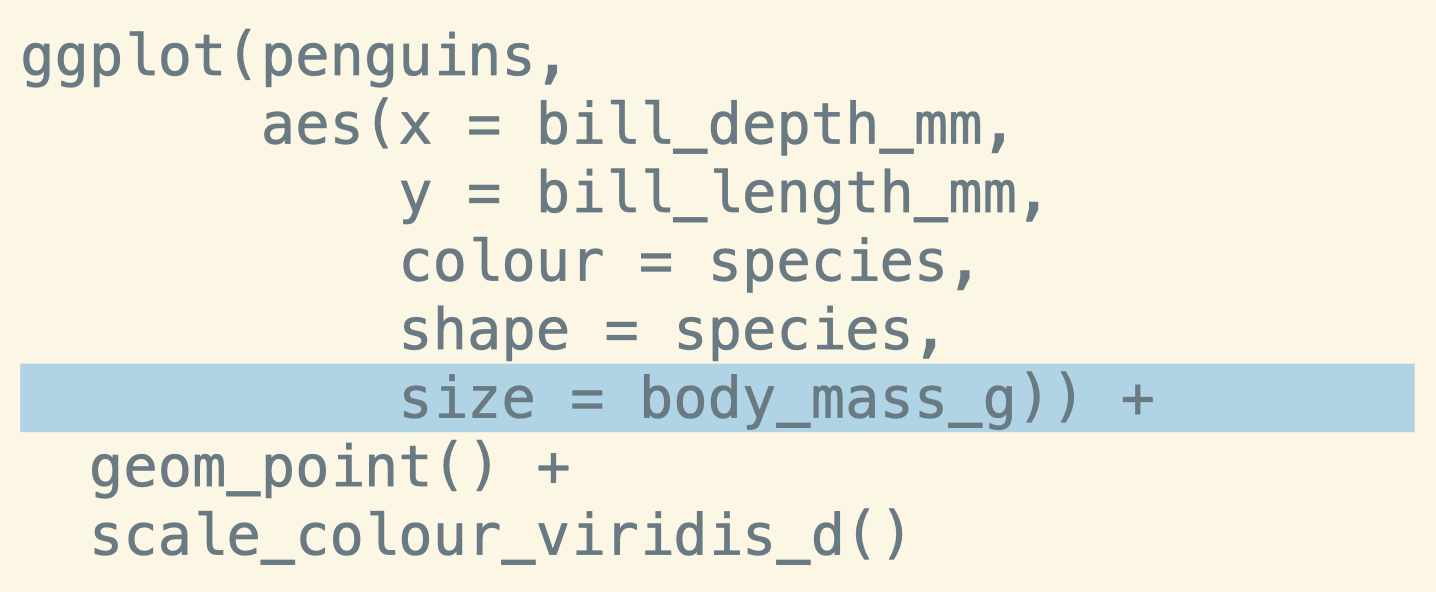
\includegraphics[width=1\linewidth]{Images/S2/code/s20}
			
		\end{figure}
	\end{minipage}%
	\begin{minipage}[t]{0.5\linewidth}
		
		\begin{figure}
			\centering
			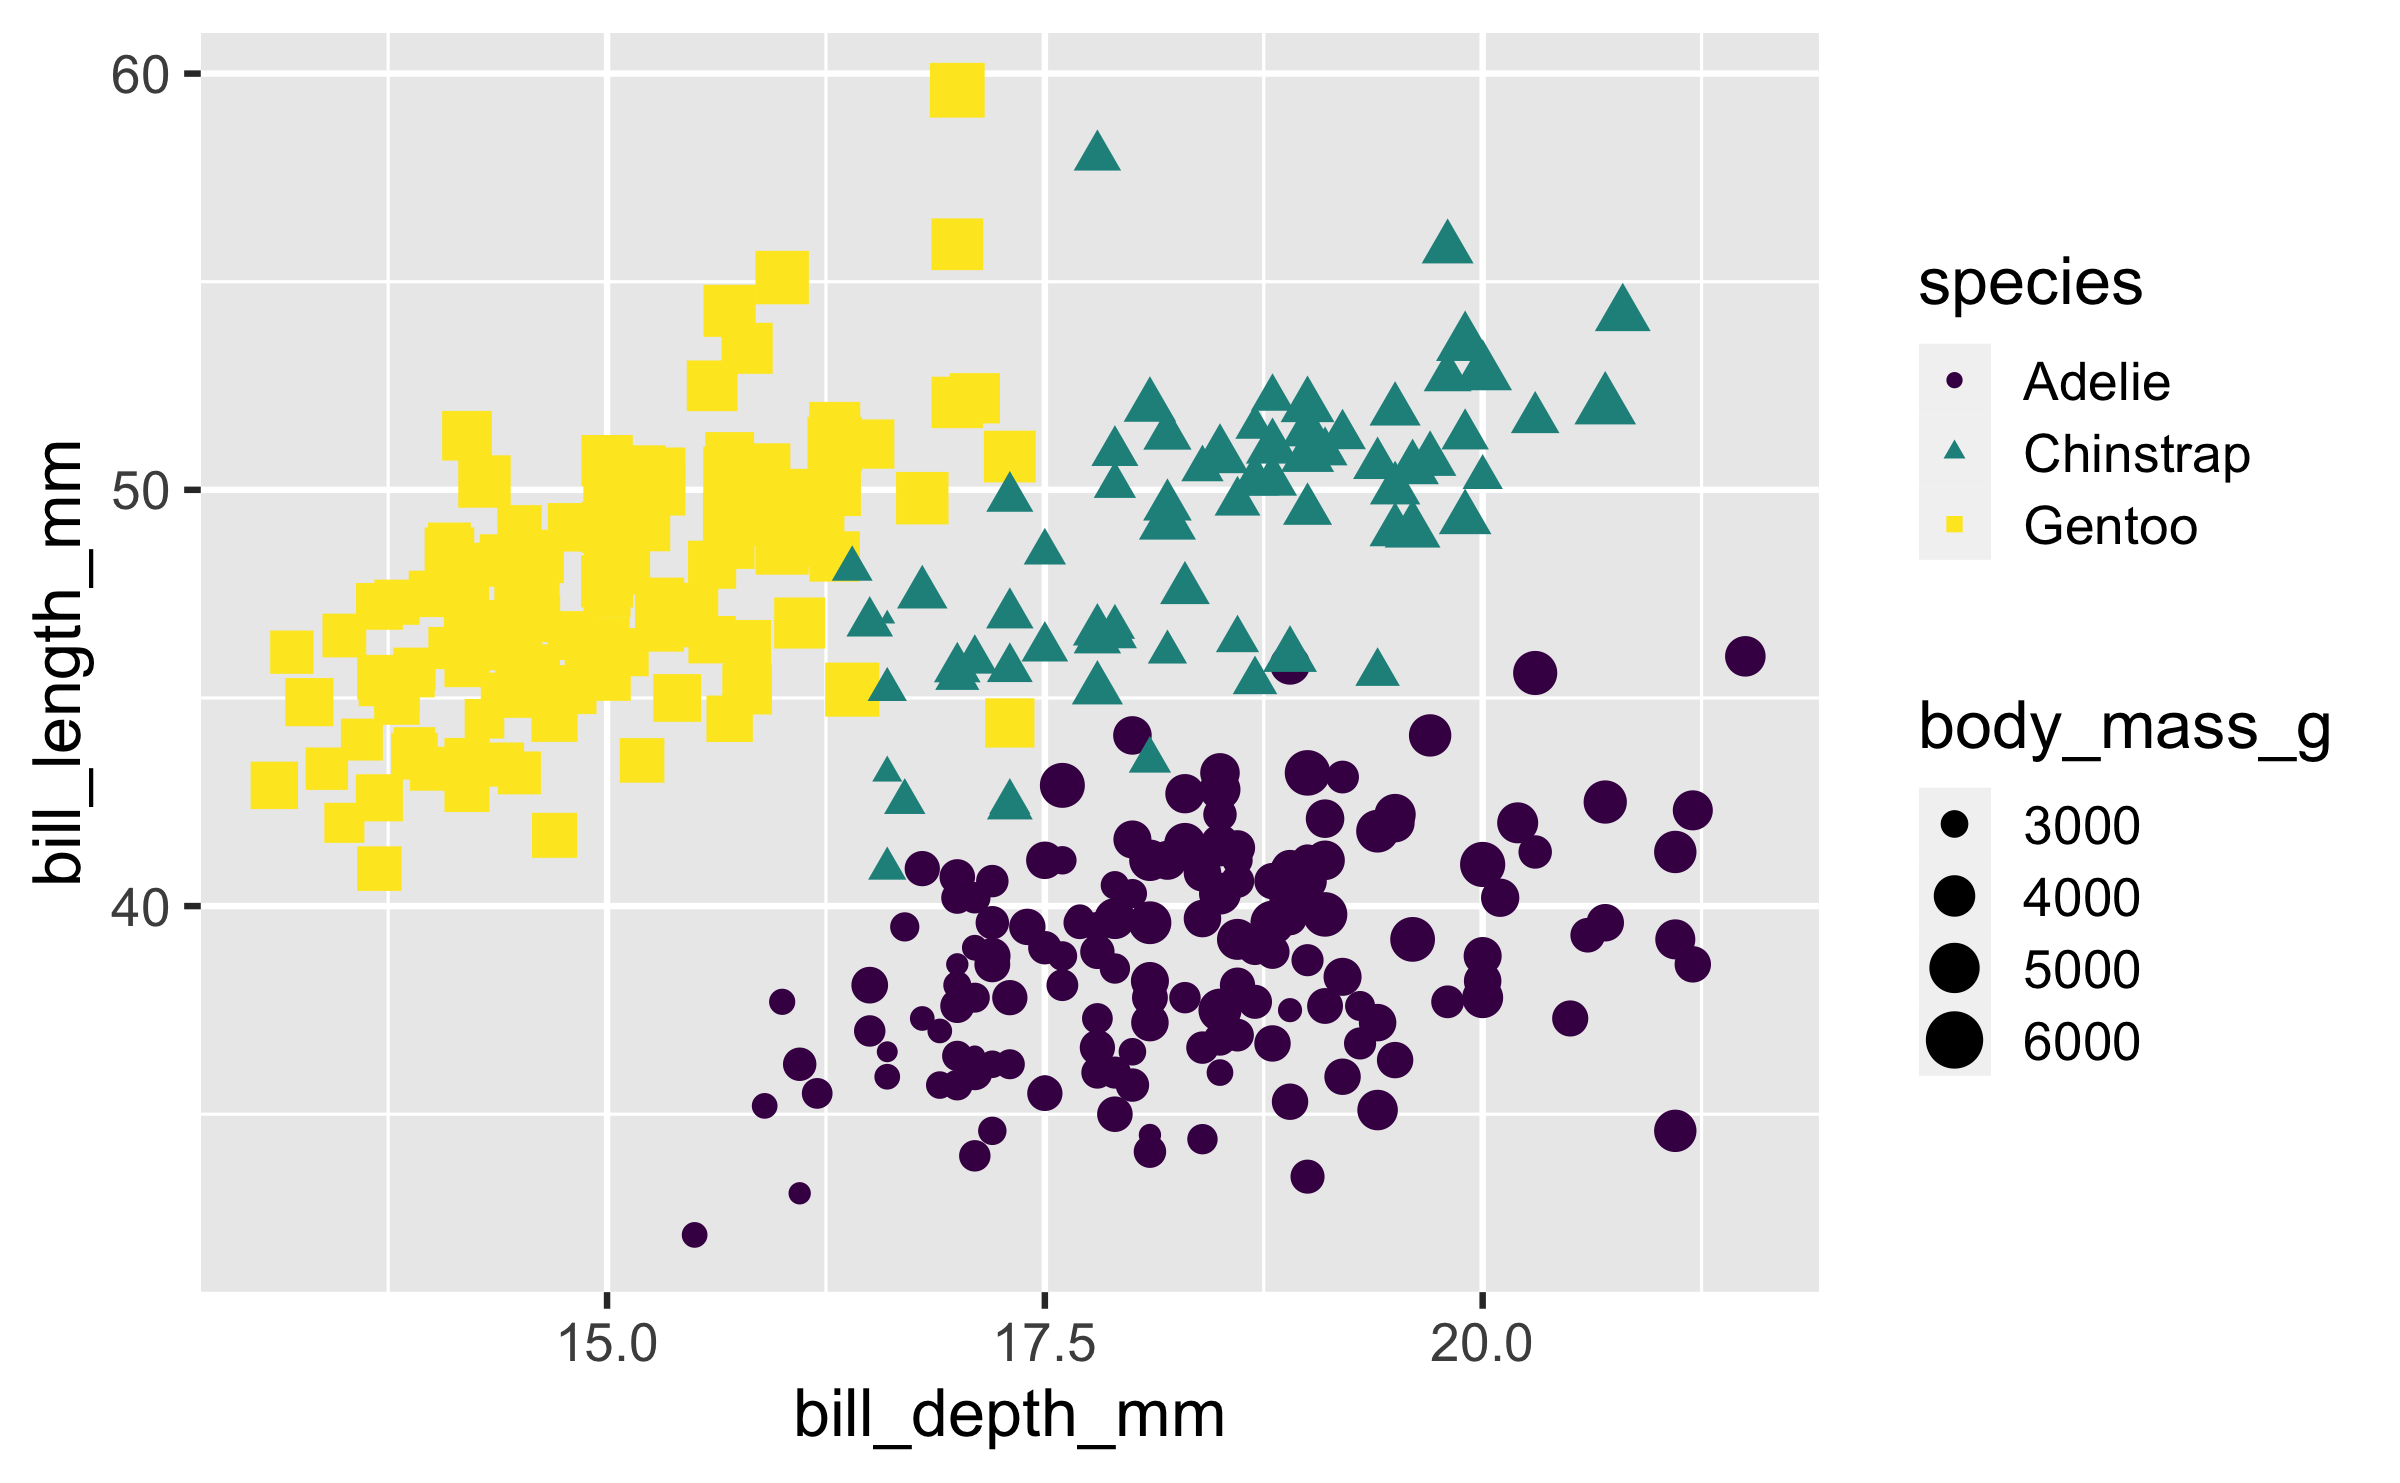
\includegraphics[width=1\linewidth]{Images/S2/size-1}
			
		\end{figure}
		
		
	\end{minipage}
	
	
\end{frame}
%------------------------------------------------------------------%

\begin{frame}
	\frametitle{\textbf{Alpha}}
	Mapped to a different variable than colour
	
	\begin{minipage}[t]{0.5\linewidth}
		\begin{figure}
			\centering
			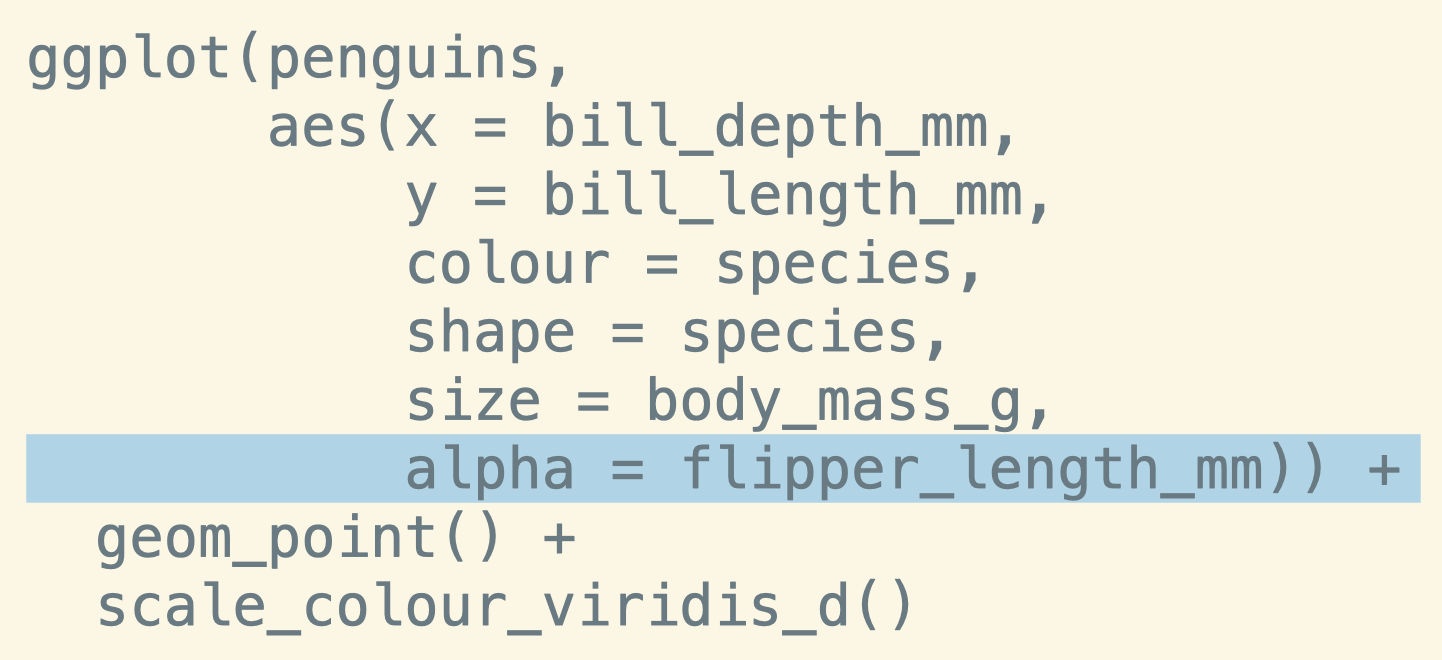
\includegraphics[width=1\linewidth]{Images/S2/code/s21}
			
		\end{figure}
	\end{minipage}%
	\begin{minipage}[t]{0.5\linewidth}
		
		\begin{figure}
			\centering
			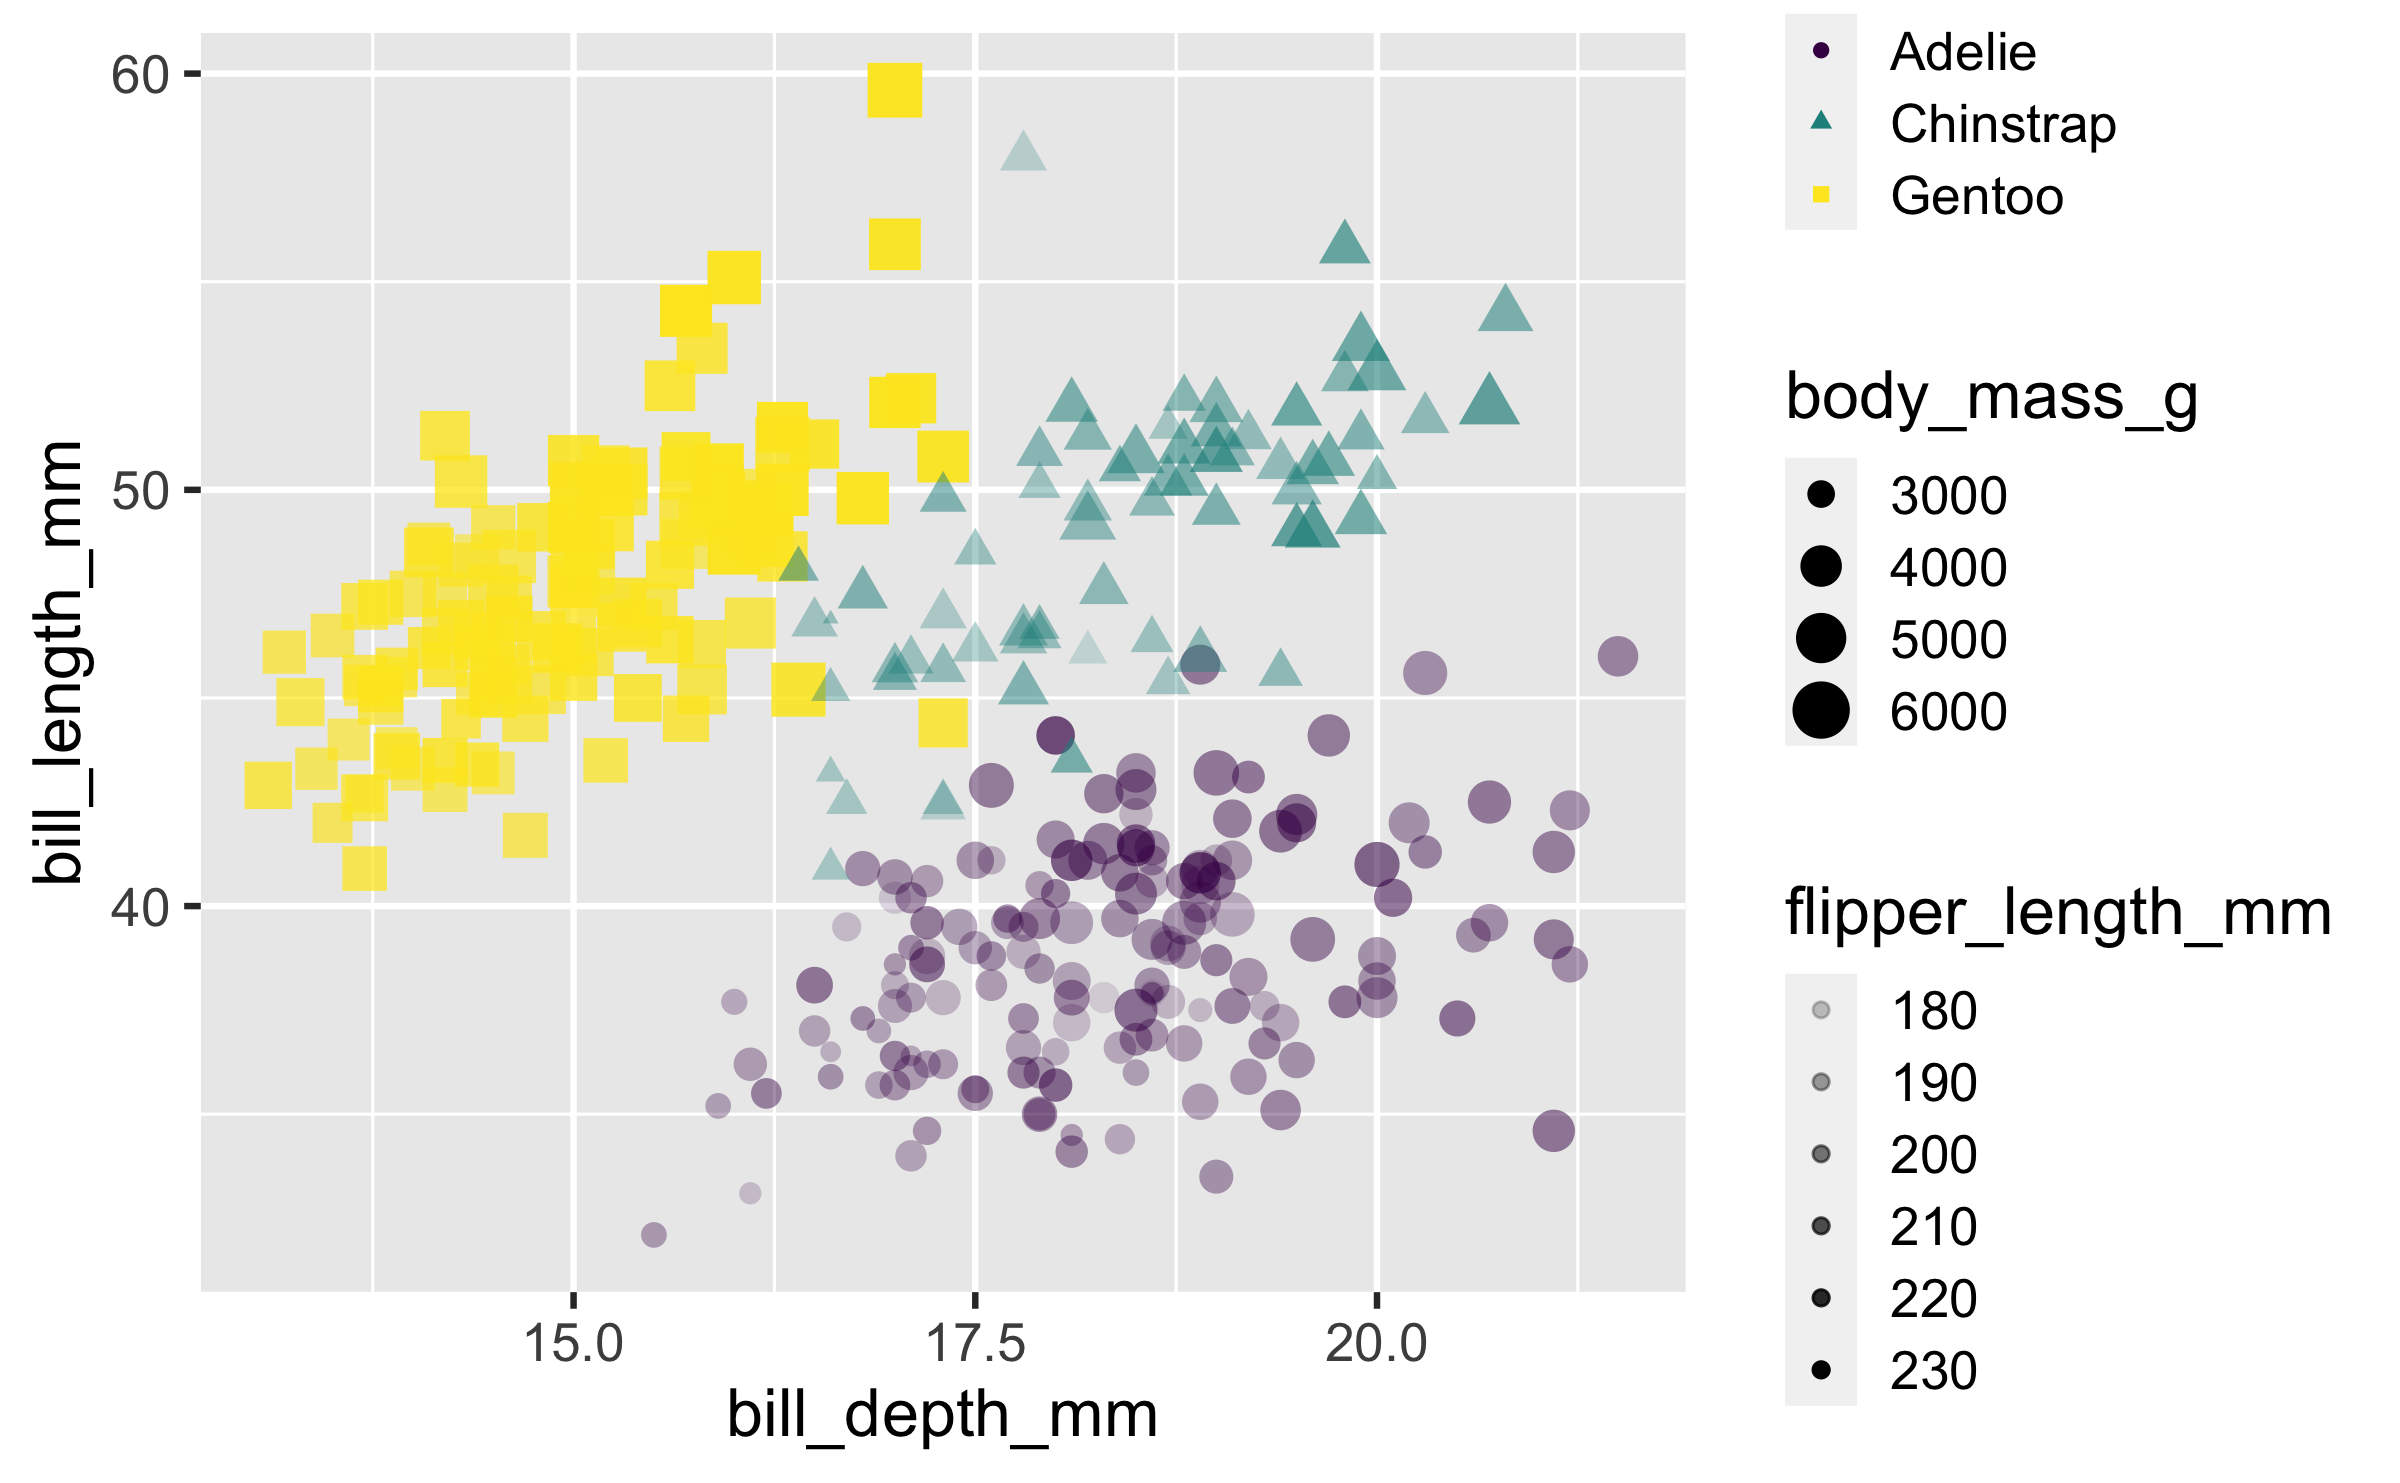
\includegraphics[width=1\linewidth]{Images/S2/alpha-1}
			
		\end{figure}
		
		
	\end{minipage}
	
	
\end{frame}
%------------------------------------------------------------------%
\begin{frame}
	\frametitle{\textbf{Mapping vs. Setting}}
	Mapped to a different variable than colour
	
	\begin{itemize}
		\item Mapping: Determine the size, alpha, etc. of points based on the values of a variable in the data. Goes into \structure{aes()}
		\item Setting: Determine the size, alpha, etc. of points not based on the values of a variable in the data. Goes into \structure{geom\_*()} 
	\end{itemize}
	
\end{frame}
%------------------------------------------------------------------%
\begin{frame}
	\frametitle{\textbf{Alpha}}
	Mapped to a different variable than colour
	
	\begin{minipage}[t]{0.5\linewidth}
		\begin{figure}
			\centering
			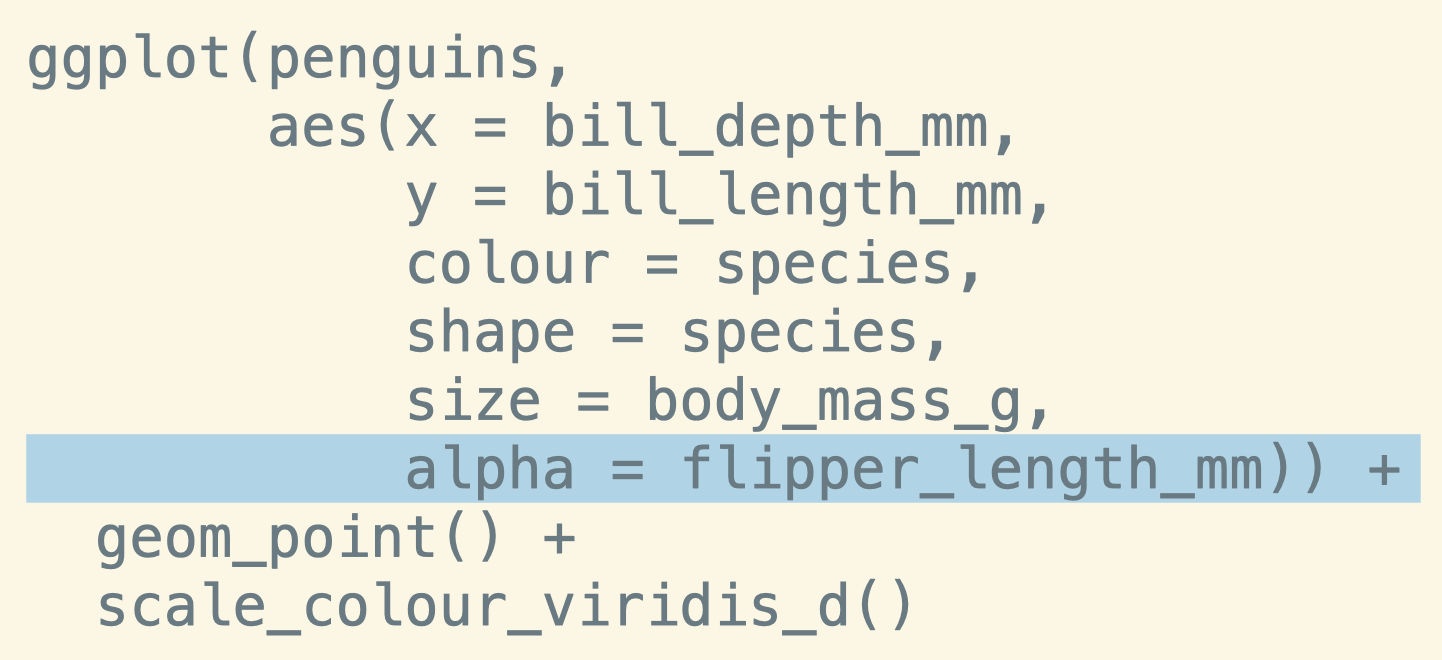
\includegraphics[width=1\linewidth]{Images/S2/code/s21}
			
		\end{figure}
	\end{minipage}%
	\begin{minipage}[t]{0.5\linewidth}
		
		\begin{figure}
			\centering
			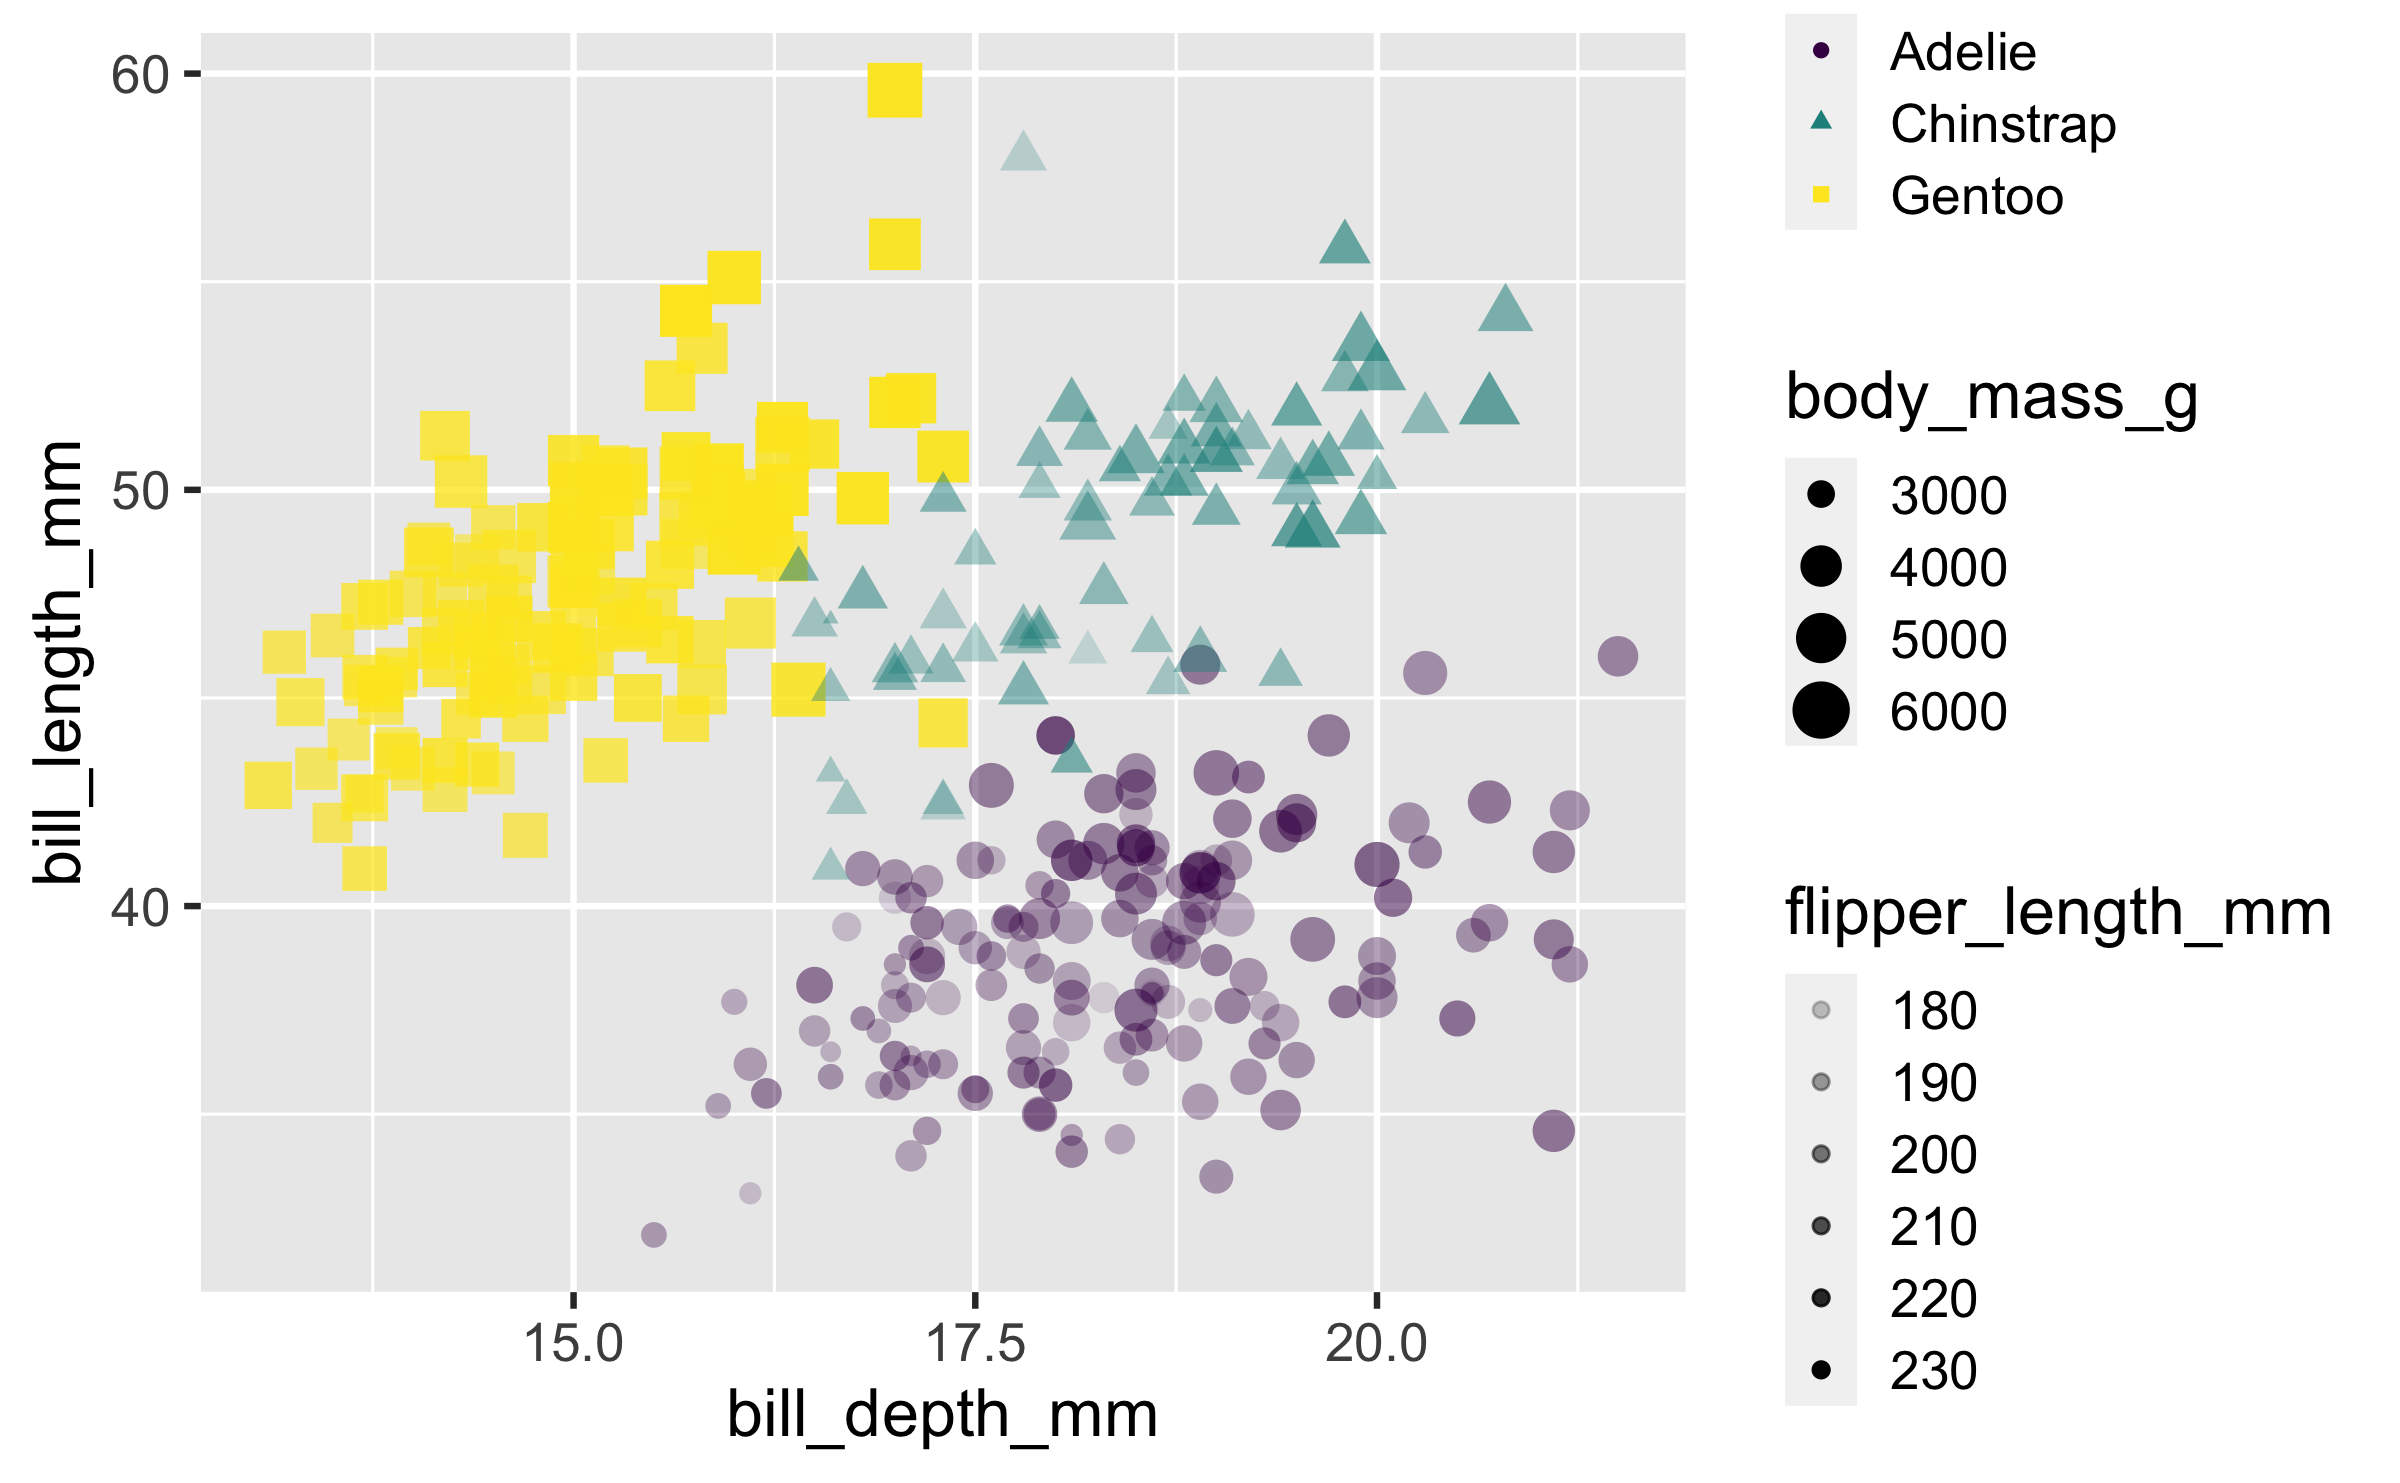
\includegraphics[width=1\linewidth]{Images/S2/alpha-1}
			
		\end{figure}
		
		
	\end{minipage}
	
	
\end{frame}
%------------------------------------------------------------------%


%------------------------------------------------------------------%

\end{document}